\documentclass[11pt,oneside,openany]{book}
\newcommand{\ShortTitle}{CATALAN / THE ARITHMETIC STILL REQUIRED}
\usepackage[T1]{fontenc}
\usepackage[utf8]{inputenc}
\usepackage{mathpazo}
\usepackage[scaled=0.92]{helvet}
\usepackage{courier}
\usepackage{amsmath,amssymb,amsthm,mathtools}
\usepackage[a4paper,left=27mm,right=27mm,top=26mm,bottom=27mm,headheight=15pt]{geometry}
\usepackage{microtype}
\usepackage{graphicx}
\usepackage[dvipsnames]{xcolor}
\usepackage{booktabs,array,longtable,tabularx}
\usepackage{enumitem}
\usepackage{titlesec,fancyhdr}
\usepackage{caption}
\usepackage{hyperref}
\definecolor{Ink}{HTML}{243138}
\definecolor{Teal}{HTML}{21676B}
\definecolor{Copper}{HTML}{A45C36}
\definecolor{Soft}{HTML}{E9F0EF}
\definecolor{Gray}{HTML}{627078}
\hypersetup{colorlinks=true,linkcolor=Teal,citecolor=Teal,urlcolor=Teal,pdfauthor={Komorebi P.}}
\urlstyle{same}
\setlength{\parindent}{1.2em}
\setlength{\parskip}{0.15em}
\linespread{1.09}
\setlist{itemsep=0.22em,topsep=0.45em,leftmargin=1.55em}
\setlist[description]{style=nextline,leftmargin=0pt,labelwidth=0pt,labelsep=0pt,font=\normalfont\bfseries}
\setcounter{tocdepth}{2}
\setlength{\emergencystretch}{1.4em}
\titleformat{\section}{\Large\bfseries\color{Ink}}{\thesection}{0.7em}{}
\titleformat{\subsection}{\large\bfseries\color{Ink}}{\thesubsection}{0.7em}{}
\titleformat{\subsubsection}{\normalsize\bfseries\color{Ink}}{\thesubsubsection}{0.7em}{}
\titlespacing*{\section}{0pt}{1.8em}{0.7em}
\titlespacing*{\subsection}{0pt}{1.3em}{0.5em}
\captionsetup{font=small,labelfont={bf,color=Teal},skip=8pt}
\pagestyle{fancy}
\fancyhf{}
\fancyhead[L]{\sffamily\scriptsize\color{Gray}OPERATION KOMOREBI}
\fancyhead[R]{\sffamily\scriptsize\color{Gray}\ShortTitle}
\fancyfoot[L]{\sffamily\scriptsize\color{Gray}CONJECTURE SERIES / 9 OCTOBER 2026}
\fancyfoot[R]{\sffamily\small\color{Ink}\thepage}
\renewcommand{\headrulewidth}{0.25pt}
\renewcommand{\footrulewidth}{0pt}
\theoremstyle{plain}
\newtheorem{theorem}{Theorem}[section]
\newtheorem{proposition}[theorem]{Proposition}
\newtheorem{lemma}[theorem]{Lemma}
\newtheorem{corollary}[theorem]{Corollary}
\newtheorem{conjecture}[theorem]{Conjecture}
\theoremstyle{definition}
\newtheorem{definition}[theorem]{Definition}
\newtheorem{example}[theorem]{Example}
\theoremstyle{remark}
\newtheorem{remark}[theorem]{Remark}
\newtheorem{hypothesis}[theorem]{Hypothesis}
\numberwithin{equation}{section}
\providecommand{\N}{\mathbb N}
\providecommand{\Z}{\mathbb Z}
\providecommand{\Q}{\mathbb Q}
\providecommand{\R}{\mathbb R}
\providecommand{\C}{\mathbb C}
\providecommand{\eps}{\varepsilon}
\providecommand{\dd}{\mathrm d}
\providecommand{\norm}[1]{\left\lVert #1\right\rVert}
\providecommand{\abs}[1]{\left\lvert #1\right\rvert}
\graphicspath{{../shared/figures/}}
\newcommand{\figplaceholder}[2]{\begin{figure}[tbp]\centering\includegraphics[width=0.97\linewidth]{#1.pdf}\caption{#2}\label{fig:#1}\end{figure}}
\newcommand{\Cover}[4]{%
\hypersetup{pageanchor=false}
\begin{titlepage}\thispagestyle{empty}
\noindent{\sffamily\small\color{Teal}OPERATION KOMOREBI\hfill CONJECTURE SERIES #1}\par
\vspace{27mm}
\noindent{\fontsize{43}{47}\selectfont\color{Ink}#2}\par
\vspace{5mm}\noindent{\LARGE\color{Ink}#3}\par
\vspace{9mm}\noindent{\color{Teal}\rule{\linewidth}{1.1pt}}\par
\vspace{8mm}\noindent{\large Komorebi P.}\par
\vspace{2mm}\noindent{\sffamily\small\color{Gray}READER EDITION 1.0 / 9 OCTOBER 2026}\par
\vfill
\noindent\begin{minipage}{0.96\linewidth}{\large\color{Ink}#4}\end{minipage}\par
\vspace{9mm}\noindent{\sffamily\small\color{Teal}EXACT IDENTITIES\quad /\quad FINITE EVIDENCE\quad /\quad OPEN CONJECTURE}\par
\end{titlepage}\hypersetup{pageanchor=true}}

\usepackage[most]{tcolorbox}
\usepackage{float,listings,calc,needspace}
\lstset{basicstyle=\ttfamily\footnotesize,breaklines=true,columns=fullflexible}
\titleformat{\chapter}[display]{\Huge\bfseries\color{Ink}\raggedright\hyphenpenalty=10000\exhyphenpenalty=10000}{\sffamily\small\color{Teal}CHAPTER \thechapter}{8pt}{}
\titlespacing*{\chapter}{0pt}{0pt}{20pt}
\counterwithout{theorem}{section}
\counterwithin{theorem}{chapter}
\counterwithout{equation}{section}
\numberwithin{equation}{chapter}
\newtheorem{problem}[theorem]{Problem}
\newtheorem{construction}[theorem]{Construction}
\newcommand{\vTwo}{\operatorname{v}_2}
\newcommand{\lcm}{\operatorname{lcm}}
\newcommand{\sgn}{\operatorname{sgn}}
\newcommand{\den}{\operatorname{den}}
\newcommand{\Span}{\operatorname{span}}
\newtcolorbox{claimboundary}{colback=Soft,colframe=Copper,title=Claim boundary,fonttitle=\bfseries,breakable,boxrule=0.7pt,arc=1mm}
\newtcolorbox{resultbox}[1][]{colback=Soft,colframe=Teal,title={#1},fonttitle=\bfseries,breakable,boxrule=0.7pt,arc=1mm}
\newtcolorbox{openproblem}[1][]{colback=white,colframe=Copper,title={#1},fonttitle=\bfseries,breakable,boxrule=0.7pt,arc=1mm}
\renewcommand{\arraystretch}{1.13}
\graphicspath{{../visual/figures/}}
\makeatletter
\renewcommand{\l@section}{\@dottedtocline{1}{1.5em}{3.6em}}
\renewcommand{\l@subsection}{\@dottedtocline{2}{5.1em}{4.2em}}
\makeatother
\hypersetup{pdftitle={Catalan's constant: the arithmetic still required},pdfsubject={Operation Komorebi, Conjecture Series 08. Mathematical reader and reproducible evidence.}}
\begin{document}
\frontmatter
\Cover{08}{Catalan's\\constant}{The arithmetic still required}{A mathematical reader on exact recurrence identities, integer packets, filtered approximations, primitive content and the remaining irrationality criterion.}
\chapter*{The question behind the calculations}
\addcontentsline{toc}{chapter}{The question behind the calculations}
Catalan's constant has a simple definition,
\[
G=\sum_{k=0}^{\infty}\frac{(-1)^k}{(2k+1)^2}.
\]
It is easy to locate on the real line. It is much harder to classify arithmetically. An accurate decimal approximation does not decide whether the value is rational. A recurrence that produces astonishingly close rational approximations does not decide that question either, unless the denominators and the nonzero errors satisfy the right bounds.

This reader follows that distinction through the recovered Operation Komorebi work. Its starting point is a small exact arithmetic program with three historical records dated 23 September 2026. The program checks a Wronskian identity, scans the powers of two dividing binomial packet sums, and computes common divisors of cleared coefficient pairs. The mathematical exposition here is newly assembled for this edition. No earlier written Catalan proof manuscript was recovered.

\begin{claimboundary}
This edition does not establish the irrationality of Catalan's constant. It supplies written arguments for specified recurrence and packet identities, checks external inputs in their exact normalization, reproduces finite arithmetic, and states the uniform estimates that would complete this route.
\end{claimboundary}

The strongest statements in the reader have different kinds of support. The Wronskian has an elementary proof valid for every index. The integrality of the scaled first coefficient follows from an authenticated binomial formula and a written coefficient argument. Even filter indices give nonzero error through a positive integral. Those statements should be stated plainly. The large divisibility scan is exact on its finite grid, and its grid should be stated just as plainly. It does not control all later indices.

\section*{How the route would finish}
If $G=a/b$ were rational, every nonzero form $AG-B$ with integers $A,B$ would have absolute value at least $1/b$. Thus nonzero integer forms tending to zero would contradict rationality. The recurrence gives small real errors. Clearing its rational coefficients multiplies those errors by an arithmetic cost. Common divisors can reduce that cost, but a divisor created by an unnecessarily large clearing factor is not itself a new saving. The crucial quantity is the error after the coefficients have been reduced.

The reader first develops the constant and this rationality obstruction. It then follows the recurrence, the Wronskian, the integer packet and the filter. The last chapters measure primitive content and make the remaining asymptotic inequality explicit. A separate visual guide follows the same route with scientific diagrams and bounded data.

\section*{A dated view of the literature}
The edition date matters. A September 2026 preprint by Zhi-Wei Sun claims an irrationality proof. A later primary note by Dane Wachs identifies an incomplete derivation involving the contribution from the prime two. Both are recorded in their checked versions. This reader does not referee every possible repair of that claim, and it does not infer rationality from a criticism of one argument. No irrationality proof is established by the material checked for this publication.

The older recurrence literature also contains a normalization discrepancy worth exposing. A printed integral prefactor conflicts with the initial value. Evaluating the first integral and comparing exact formal coefficients prevents that mismatch from entering the packet calculations. The source contracts record both the printed formula and the normalization actually used here.

\section*{Evidence and reproducibility}
The source bundle contains the three historical records byte for byte, the current LaTeX, the Python figures, fresh run manifests, and separate mathematical, source and layout audits. The historical default output was reproduced byte for byte. An additional implementation compared every pair in the smaller direct grid, rather than comparing only the observed maxima.

An exploratory sign rule for odd filters failed. That failure is retained with an exact counterexample. The restriction to even filter indices has a written nonvanishing argument, so the failed guess need not be disguised or treated as fatal to the entire construction.

Neither repeated computational agreement nor agreement between reviewers is a universal proof. No proof assistant certification is claimed. The purpose of the release is to make the conclusions, dependencies and remaining work concrete enough to inspect and reproduce.

\medskip
\noindent\textbf{Komorebi P.}\\
Operation Komorebi\\
Reader edition 1.0, 9 October 2026

{\small\linespread{1}\selectfont\setlength{\parskip}{0pt}\tableofcontents}
\mainmatter
\chapter{A constant with many exact faces}
\label{ch:constant}

Catalan's constant begins with an unusually accessible definition. Its terms are rational, their signs alternate, and its value can be enclosed without assuming anything about irrationality. The difficulty appears when one asks what kind of number the limit is. A definition, an integral, a recurrence and a long decimal expansion each give access to the same number. None of these descriptions alone supplies the arithmetic conclusion.

This chapter fixes the analytic object before we introduce rational approximants. All integral identities and interval bounds below are proved directly. The finite computations in the accompanying bundle use these bounds to decide signs. They do not use a floating point approximation to make an exact decision.

\section{Definition and the question being asked}

\begin{definition}[Catalan's constant]
\label{def:c01-G}
The real number studied in this book is
\begin{equation}
G=\sum_{k=0}^{\infty}\frac{(-1)^k}{(2k+1)^2}.
\label{eq:c01-definition}
\end{equation}
The series converges absolutely because
\[
\sum_{k=0}^{\infty}\frac1{(2k+1)^2}
\leq\sum_{j=1}^{\infty}\frac1{j^2}<\infty.
\]
\end{definition}

The familiar decimal display begins
\[
G\approx0.91596559417721901505460351493238411077.
\]
The approximation sign matters. A decimal is a coordinate for seeing the number, while a rational enclosure is evidence for a particular numerical assertion. A proof of irrationality requires a different assertion again.

\begin{conjecture}[The irrationality question]
\label{conj:c01-irrationality}
Catalan's constant does not belong to $\Q$.
\end{conjecture}

The checked material for this edition does not establish this conjecture. The literature record includes a September 2026 preprint claiming a proof and a subsequent primary note identifying an incomplete asymptotic derivation \cite{Sun2026,Wachs2026}. The later chapters state that record with its date and scope. The constructions developed here do not depend on accepting the claimed proof.

Irrationality would mean that no integers $a,b$ with $b\ne0$ satisfy $G=a/b$. Transcendence would mean that no nonzero polynomial with integer coefficients vanishes at $G$. These are different questions. The second implies the first, because a rational number $a/b$ is a zero of the polynomial $bx-a$. Our target throughout is the first assertion.

\begin{figure}[tbp]
\centering
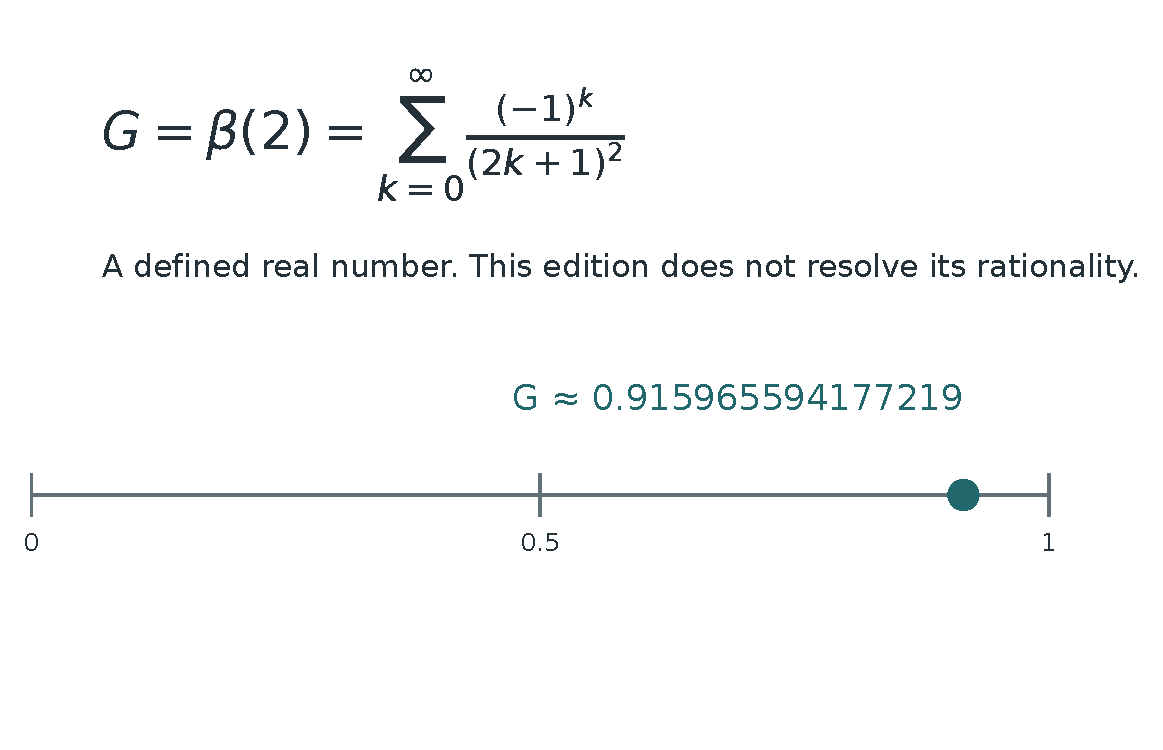
\includegraphics[width=0.94\linewidth]{../visual/figures/01_constant.pdf}
\caption{The same constant appears through a convergent series and through exact integral representations. The displayed decimal supplies orientation. The formulas, rather than the printed digits, define the object.}
\label{fig:c01-constant}
\end{figure}

\subsection{The Dirichlet beta family}

For real $s>1$, the Dirichlet beta value is
\begin{equation}
\beta(s)=\sum_{k=0}^{\infty}\frac{(-1)^k}{(2k+1)^s}.
\label{eq:c01-beta}
\end{equation}
Absolute convergence follows from comparison with $\sum j^{-s}$. Thus $G=\beta(2)$. The alternating series also defines $\beta(s)$ for $s>0$, though absolute convergence is no longer available throughout that wider range. At $s=1$, integration of the finite geometric expansion of $(1+x^2)^{-1}$ gives $\beta(1)=\pi/4$. The integrated remainder is bounded by $\int_0^1x^{2N}\dd x=(2N+1)^{-1}$ and tends to zero, so this passage does not require absolute convergence of the beta series at $1$.

The family gives useful context without collapsing its separate arithmetic questions. Zudilin proved that at least one of
\[
\beta(2),\ \beta(4),\ \beta(6),\ \beta(8),\ \beta(10),\ \beta(12)
\]
is irrational \cite{Zudilin2019}. This is a disjunction. It permits the irrational member to be a value other than $\beta(2)$. A proof about the collection therefore cannot be inserted as a proof about $G$. The precise source contract is LC09 in the evidence bundle.

\section{Alternating partial sums give rational intervals}

Write
\begin{equation}
s_N=\sum_{k=0}^{N-1}\frac{(-1)^k}{(2k+1)^2},\qquad N\geq0,
\label{eq:c01-partial-sum}
\end{equation}
where $s_0=0$ is the empty sum. Thus $N$ counts retained terms, as it does in the visual guide. Each $s_N$ is an exact rational number. The terms decrease strictly in magnitude to zero. Grouping successive terms shows that the even partial sums increase and the odd partial sums decrease. These two sequences approach the same limit.

\begin{proposition}[Alternating enclosure]
\label{prop:c01-alternating}
For every integer $r\geq0$,
\begin{equation}
s_{2r}<G<s_{2r+1}.
\label{eq:c01-parity-enclosure}
\end{equation}
For every integer $N\geq0$,
\begin{equation}
0<(-1)^N(G-s_N)<\frac1{(2N+1)^2}.
\label{eq:c01-alternating-error}
\end{equation}
\end{proposition}

\begin{proof}
The difference between two consecutive even sums is
\[
s_{2r+2}-s_{2r}
=\frac1{(4r+1)^2}-\frac1{(4r+3)^2}>0.
\]
Similarly,
\[
s_{2r+3}-s_{2r+1}
=-\frac1{(4r+3)^2}+\frac1{(4r+5)^2}<0.
\]
Consecutive sums differ by a term tending to zero, so the increasing even sums and decreasing odd sums have the same limit $G$. Strictness follows because the next sum of the same parity lies strictly between the current endpoint and the limit on the other side.

To obtain the error bound, apply this enclosure to $s_N$ and $s_{N+1}$. The limit lies strictly between them. Their distance is $(2N+1)^{-2}$, and the direction from $s_N$ to $s_{N+1}$ has sign $(-1)^N$.
\end{proof}

For example,
\[
s_0=0,\qquad s_1=1,\qquad s_2=\frac89,\qquad
s_3=\frac{209}{225},\qquad
s_4=\frac{10016}{11025}.
\]
Hence
\begin{equation}
\frac{10016}{11025}<G<\frac{209}{225}.
\label{eq:c01-small-bracket}
\end{equation}
These statements use only rational arithmetic. The strict inequality also proves $0<G<1$, which will simplify later tail estimates.

\begin{figure}[tbp]
\centering
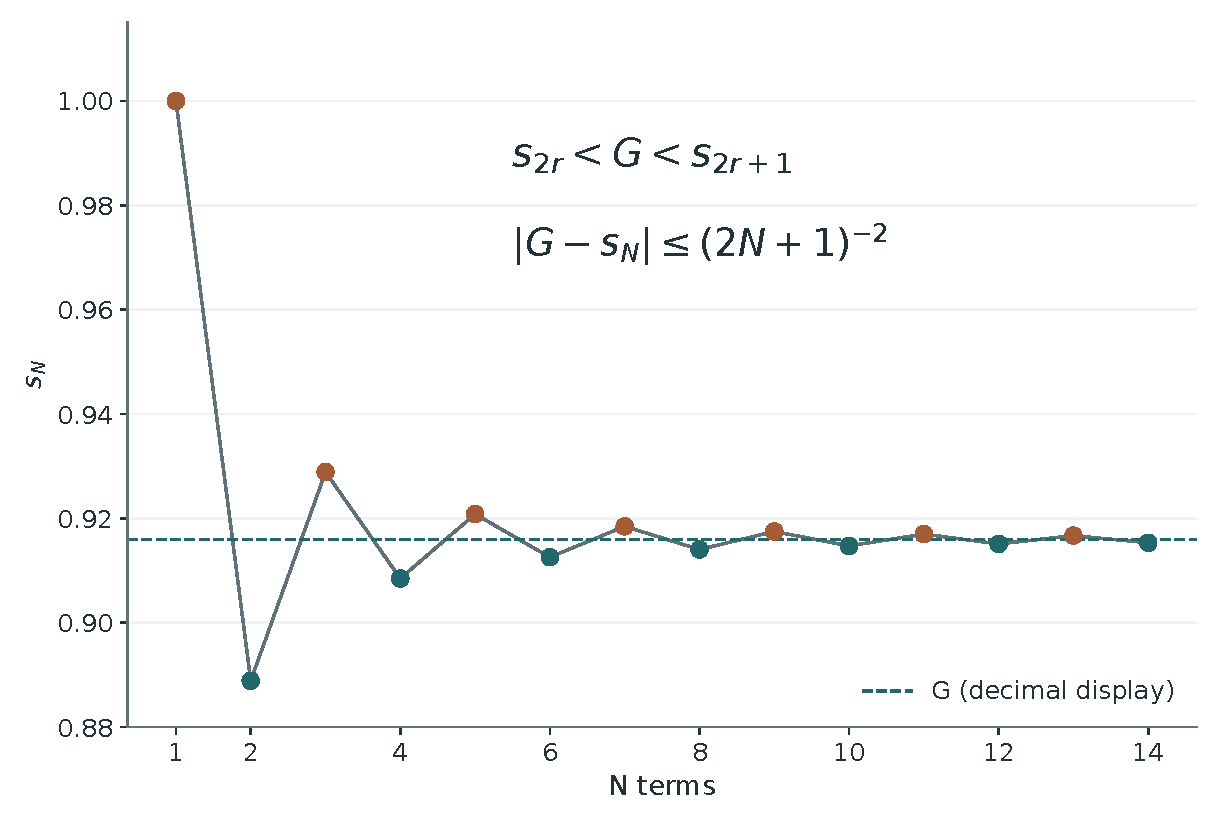
\includegraphics[width=0.94\linewidth]{../visual/figures/02_alternating_series.pdf}
\caption{Even and odd partial sums approach the common limit from opposite sides. Their errors are controlled by the next omitted term. Every partial sum represented in the figure is rational.}
\label{fig:c01-alternating}
\end{figure}

The error bound is transparent, but its decay is slow. To make the next omitted term smaller than $10^{-d}$, one needs $2N+1>10^{d/2}$. Increasing numerical accuracy this way rapidly becomes expensive. The Euler transform below produces a much faster certified enclosure. Before using it, we establish the positive integral that controls its terms.

\section{Three exact integral descriptions}

\subsection{A logarithmic integral}

\begin{lemma}[A basic moment]
\label{lem:c01-moment}
For every real $a>-1$,
\begin{equation}
\int_0^1x^a(-\log x)\,\dd x=\frac1{(a+1)^2}.
\label{eq:c01-moment}
\end{equation}
The integral is understood as an improper integral at $0$.
\end{lemma}

\begin{proof}
Set $x=e^{-t}$. Then $-\log x=t$, $\dd x=-e^{-t}\dd t$, and the integral becomes
\[
\int_0^{\infty}t e^{-(a+1)t}\,\dd t.
\]
Integration by parts gives $(a+1)^{-2}$. The boundary term at infinity is zero because an exponential with positive decay rate dominates $t$. The boundary term at zero is also zero.
\end{proof}

\begin{proposition}[Single integral]
\label{prop:c01-log-integral}
Catalan's constant satisfies
\begin{equation}
G=\int_0^1\frac{-\log x}{1+x^2}\,\dd x.
\label{eq:c01-log-integral}
\end{equation}
\end{proposition}

\begin{proof}
For $0\leq x<1$, the geometric expansion is
\[
\frac1{1+x^2}=\sum_{k=0}^{\infty}(-1)^kx^{2k}.
\]
The integrated absolute values of the proposed terms have finite sum:
\[
\sum_{k=0}^{\infty}\int_0^1x^{2k}(-\log x)\,\dd x
=\sum_{k=0}^{\infty}\frac1{(2k+1)^2}<\infty.
\]
Therefore the series of integrable functions can be summed under the integral. The moment identity gives the defining series for $G$. The point $x=1$ has measure zero and does not affect the integral.
\end{proof}

The singularity in $-\log x$ is integrable. This is a useful example of why an unbounded integrand is not the same as an infinite integral. In fact, $\int_0^1-\log x\,\dd x=1$. The factor $(1+x^2)^{-1}$ is bounded between $1/2$ and $1$, so the integral representation independently places $G$ between $1/2$ and $1$.

\subsection{An arctangent and a logarithmic tangent}

\begin{proposition}[Arctangent and tangent forms]
\label{prop:c01-tangent}
The following equalities hold:
\begin{equation}
G=\int_0^1\frac{\arctan x}{x}\,\dd x
=-\int_0^{\pi/4}\log(\tan\theta)\,\dd\theta.
\label{eq:c01-tangent-forms}
\end{equation}
The integrand $\arctan x/x$ is assigned its continuous value $1$ at $x=0$.
\end{proposition}

\begin{proof}
For $0<\delta<1$, integration by parts gives
\[
\int_\delta^1\frac{\arctan x}{x}\,\dd x
=-\arctan(\delta)\log\delta
-\int_\delta^1\frac{\log x}{1+x^2}\,\dd x.
\]
The boundary expression tends to zero as $\delta\downarrow0$, since $0\leq\arctan\delta\leq\delta$ and $\delta\abs{\log\delta}\to0$. The first equality follows from Proposition~\ref{prop:c01-log-integral}.

For the second equality, substitute $x=\tan\theta$ into the logarithmic integral. On $0<\theta\leq\pi/4$,
\[
\frac{\dd x}{1+x^2}=\dd\theta.
\]
The substitution is valid first on a truncated interval. Its limit exists by the integrability already established for $-\log x$.
\end{proof}

The logarithmic tangent form will later identify an integral normalization at index zero. That check is especially valuable because a constant factor in a linear form changes its normalization even when its qualitative decay is unaffected. We will use the equality just proved, rather than assume the normalization from a printed formula.

\subsection{A double integral over a square}

\begin{proposition}[Elementary double integral]
\label{prop:c01-double}
Catalan's constant also satisfies
\begin{equation}
G=\int_0^1\int_0^1\frac{\dd x\,\dd y}{1+x^2y^2}.
\label{eq:c01-double}
\end{equation}
\end{proposition}

\begin{proof}
One proof integrates with respect to $y$. For $x>0$,
\[
\int_0^1\frac{\dd y}{1+x^2y^2}=\frac{\arctan x}{x}.
\]
The value at $x=0$ is $1$. Proposition~\ref{prop:c01-tangent} now gives the result.

There is also a direct series justification. Expanding $(1+x^2y^2)^{-1}$ on the square except at the corner $(1,1)$ gives geometric terms $(-1)^kx^{2k}y^{2k}$. Their integrated absolute values sum to
\[
\sum_{k=0}^{\infty}\left(\int_0^1x^{2k}\,\dd x\right)^2
=\sum_{k=0}^{\infty}\frac1{(2k+1)^2}<\infty.
\]
Thus summation and integration may be interchanged, giving the defining series again.
\end{proof}

The double integral is bounded and positive on a compact square. The logarithmic integral has an integrable endpoint singularity. Both represent exactly the same number. Their different analytic forms permit different transformations, but their arithmetic classification remains a separate obligation.

\section{An Euler transform with an exact tail bound}

Let
\[
a_k=\frac1{(2k+1)^2},\qquad k\geq0,
\]
and define the positive difference convention
\begin{equation}
\Delta a_k=a_k-a_{k+1}.
\label{eq:c01-difference-convention}
\end{equation}
The sign convention is fixed here because the other common convention would change every odd difference. Iteration gives
\begin{equation}
\Delta^j a_0=\sum_{k=0}^{j}(-1)^k\binom jk\frac1{(2k+1)^2}.
\label{eq:c01-finite-difference}
\end{equation}
This is an exact rational number for every $j$.

\begin{lemma}[Positive differences]
\label{lem:c01-positive-differences}
For every integer $j\geq0$,
\begin{equation}
\Delta^j a_0
=\int_0^1(1-x^2)^j(-\log x)\,\dd x,
\qquad 0<\Delta^j a_0\leq1.
\label{eq:c01-positive-differences}
\end{equation}
\end{lemma}

\begin{proof}
Insert the moment formula into the finite sum in \eqref{eq:c01-finite-difference}. A finite sum can be interchanged with an integral without any convergence issue. The binomial theorem gives
\[
\sum_{k=0}^{j}(-1)^k\binom jkx^{2k}=(1-x^2)^j.
\]
The integrand is positive for $0<x<1$. It is at most $-\log x$, whose integral is $1$.
\end{proof}

\begin{theorem}[Certified Euler enclosure]
\label{thm:c01-euler}
Define
\begin{equation}
E_N=\sum_{j=0}^{N}\frac{\Delta^j a_0}{2^{j+1}},\qquad N\geq0.
\label{eq:c01-E}
\end{equation}
Then
\begin{equation}
G=\sum_{j=0}^{\infty}\frac{\Delta^j a_0}{2^{j+1}},
\qquad
E_N<G<E_N+2^{-N-1}.
\label{eq:c01-euler-enclosure}
\end{equation}
More precisely,
\begin{equation}
G-E_N
=\int_0^1\frac{-\log x}{1+x^2}
\left(\frac{1-x^2}{2}\right)^{N+1}\,\dd x.
\label{eq:c01-euler-remainder}
\end{equation}
\end{theorem}

\begin{proof}
By the preceding lemma all terms of the series are nonnegative. Monotone convergence permits the sum to pass under the integral. For $0\leq x\leq1$,
\[
\sum_{j=0}^{\infty}\frac{(1-x^2)^j}{2^{j+1}}
=\frac1{1+x^2}.
\]
The resulting integral is $G$ by Proposition~\ref{prop:c01-log-integral}.

The finite geometric identity is
\[
\sum_{j=0}^{N}\frac{(1-x^2)^j}{2^{j+1}}
=\frac{1-((1-x^2)/2)^{N+1}}{1+x^2}.
\]
Integration gives the exact remainder formula. Its integrand is positive on $(0,1)$, so $G-E_N>0$. Since $(1-x^2)/2\leq1/2$,
\[
G-E_N\leq2^{-N-1}G<2^{-N-1}.
\]
This gives the stated enclosure. An alternative bound sums the omitted terms using $\Delta^ja_0\leq1$, with the same geometric tail $2^{-N-1}$.
\end{proof}

The stronger intermediate inequality also gives
\begin{equation}
G\leq\frac{E_N}{1-2^{-N-1}}.
\label{eq:c01-euler-sharper}
\end{equation}
The denominator is positive for every $N\geq0$. The release computations use the simpler interval $[E_N,E_N+2^{-N-1}]$, because that interval has an immediate rational width and is already sufficient for the tested signs.

\begin{example}[Small Euler intervals]
The first difference values are
\[
\Delta^0a_0=1,\qquad \Delta a_0=\frac89,\qquad
\Delta^2a_0=\frac{184}{225}.
\]
They give
\[
E_0=\frac12,\qquad E_1=\frac{13}{18},\qquad
E_2=\frac{371}{450}.
\]
Thus, for example,
\[
\frac{371}{450}<G<\frac{1709}{1800}.
\]
These short transformed sums are useful for checking conventions. Their principal advantage appears as $N$ grows, because the certified width decreases geometrically.
\end{example}

The independent audit retains $j=0,\ldots,1000$. Its exact rational endpoints differ by $2^{-1001}$. The finite differences and endpoint numerators are recorded in the evidence bundle. The preceding theorem proves the tail bound for every $N$. The program computes the finite rational portion at one chosen $N$ and checks its internal arithmetic. These are complementary forms of evidence with different scopes.

\section{What a certified interval can decide}

Suppose $l\leq G\leq h$ is a proven rational enclosure, and suppose $a,b\in\Q$. Then the interval for $aG-b$ is
\begin{equation}
\begin{cases}
[al-b,ah-b],&a\geq0,\\
[ah-b,al-b],&a<0.
\end{cases}
\label{eq:c01-linear-interval}
\end{equation}
All endpoints are rational. If the entire interval is positive, the form is positive. If the entire interval is negative, the form is negative. If it contains zero, the enclosure has not decided the sign. That last outcome is a limitation of the chosen certificate, not evidence that the form actually vanishes.

This procedure makes the finite sign checks reproducible. It also limits their interpretation. A finite family of certified nonzero forms proves nonvanishing for those forms. It does not prove a universal assertion about all indices. A long decimal expansion cannot replace the rational enclosure when a coefficient is large enough to amplify the final rounding error.

The next chapter explains why even an infinite family of nonzero real errors is not enough. Their coefficients must become integers, and the errors after that arithmetic operation must still tend to zero.

\chapter{The arithmetic threshold for irrationality}
\label{ch:lattice}

The real approximation problem asks for rational numbers near $G$. The arithmetic problem asks for nonzero integer linear forms in $G$ whose absolute values tend to zero. These problems are related, but the passage between them has a cost. A coefficient denominator can absorb the analytic gain. A common divisor can recover some of that gain. Nonvanishing has to survive the whole construction.

The threshold is elementary enough to prove in a few lines. Its applications are demanding because all its hypotheses must hold together. This chapter states the criterion precisely, gives rational counterexamples to weaker assertions, and sets up the rate accounting used for the later filters.

\section{Rational numbers leave a fixed gap}

\begin{lemma}[Rational lattice gap]
\label{lem:c02-gap}
Suppose $\alpha=a/b$ with $a\in\Z$ and $b\in\Z_{>0}$. For every pair $P,Q\in\Z$, either $Q\alpha-P=0$ or
\begin{equation}
\abs{Q\alpha-P}\geq\frac1b.
\label{eq:c02-gap}
\end{equation}
\end{lemma}

\begin{proof}
Multiplication by $b$ gives
\[
b(Q\alpha-P)=Qa-Pb\in\Z.
\]
A nonzero integer has absolute value at least $1$. Division by the positive integer $b$ gives the result. No coprimality hypothesis is needed.
\end{proof}

For a fixed rational $\alpha$, every integer form $Q\alpha-P$ lies in the discrete set $b^{-1}\Z$. Its nonzero values cannot enter the open interval $(-1/b,1/b)$. The denominator $b$ need not be known to use this obstruction. If a constructed infinite family has nonzero values tending to zero, it eventually violates the gap for any proposed $b$.

\begin{theorem}[Integer form criterion]
\label{thm:c02-criterion}
Let $\alpha\in\R$. Suppose there are integer pairs $(P_j,Q_j)$ for $j\geq1$ such that
\begin{equation}
0<\abs{Q_j\alpha-P_j}\longrightarrow0.
\label{eq:c02-form-criterion}
\end{equation}
Then $\alpha$ is irrational. The same conclusion holds if these conditions are verified along any infinite subsequence.
\end{theorem}

\begin{proof}
If $\alpha=a/b$ were rational with $b>0$, Lemma~\ref{lem:c02-gap} would bound every nonzero form below by $1/b$. This contradicts convergence to zero. Restricting to a subsequence does not change the argument.
\end{proof}

\begin{figure}[tbp]
\centering
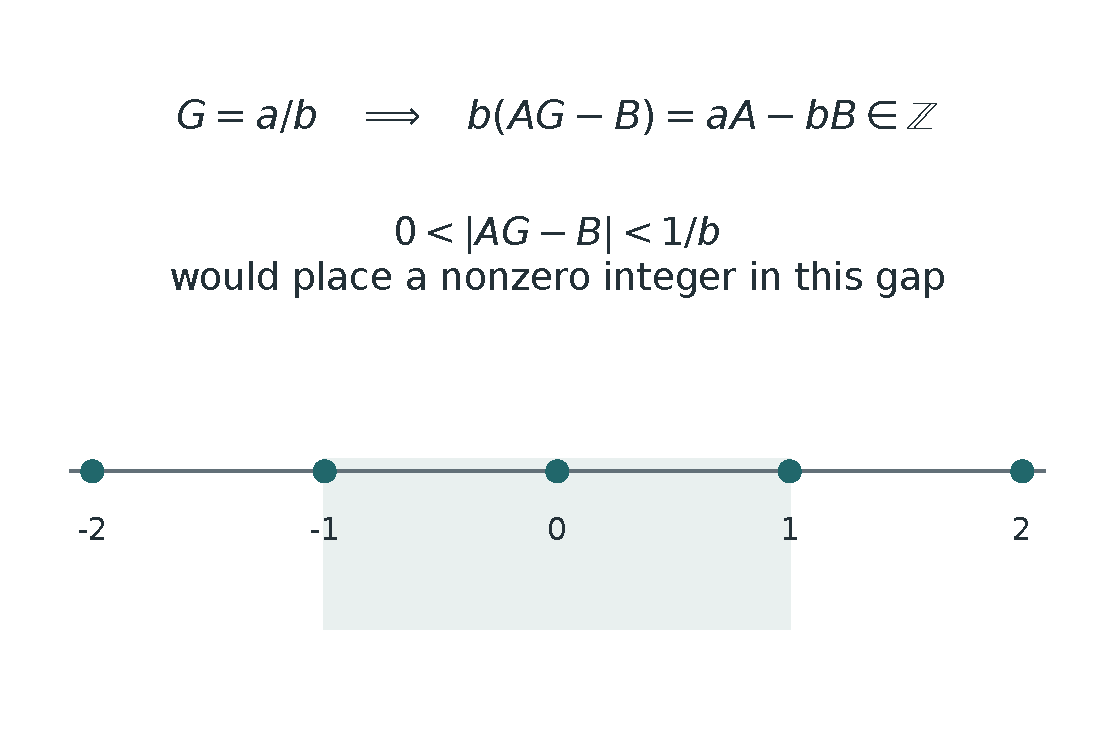
\includegraphics[width=0.94\linewidth]{../visual/figures/06_rationality_lattice.pdf}
\caption{Under the assumption $G=a/b$, integer linear forms lie on a lattice with spacing $1/b$. A sequence of nonzero forms approaching zero would contradict that spacing. The spacing is conceptual here because the hypothetical denominator is unknown.}
\label{fig:c02-lattice}
\end{figure}

The theorem separates three obligations. The coefficients must be integers. The forms must be nonzero at the indices being used. Their absolute values must approach zero. It is possible to establish any two while the third remains open.

For instance, setting $P_j=Q_j=0$ gives integer coefficients and zero error at every index, but proves nothing. Taking a rational approximation with a tiny error gives a small real form, but its coefficients may have large rational denominators. Clearing those denominators may keep the resulting integer form far from zero. These examples explain why the hypotheses are kept distinct throughout this book.

\subsection{Why the criterion is also a characterization}

The criterion is sufficient for irrationality. Conversely, every irrational real number admits such a family. This observation clarifies the role of the later constructions. The existence of small integer forms is not itself a novel definition of irrationality. The research problem is to construct and justify them for a specific constant.

\begin{proposition}[Elementary approximation by integer forms]
\label{prop:c02-pigeonhole}
If $\alpha$ is irrational, then for every integer $H\geq1$ there are integers $P,Q$ with $1\leq Q\leq H$ satisfying
\begin{equation}
0<\abs{Q\alpha-P}<\frac1H.
\label{eq:c02-pigeonhole}
\end{equation}
In particular, an infinite family as in Theorem~\ref{thm:c02-criterion} exists.
\end{proposition}

\begin{proof}
Consider the $H+1$ fractional parts of $0,\alpha,2\alpha,\ldots,H\alpha$. Partition $[0,1)$ into $H$ intervals of length $1/H$, using half open intervals. Two fractional parts lie in one interval. Their difference has absolute value strictly smaller than $1/H$. Subtracting the corresponding multiples of $\alpha$ gives $Q\alpha-P$ with $1\leq Q\leq H$ after choosing the order of the two indices.

The form is nonzero because $\alpha$ is irrational and $Q\ne0$. Choosing such a pair for every $H$ gives nonzero forms tending to zero. The denominators $Q$ cannot remain bounded. For any fixed finite set of positive $Q$, the distances from $Q\alpha$ to the nearest integers have a positive minimum. That minimum would contradict the bound as $H\to\infty$.
\end{proof}

This proof assumes irrationality in order to ensure nonvanishing. It cannot be used to prove irrationality of $G$ by inserting $\alpha=G$ before that fact is known. The lattice criterion runs in the other direction: first establish small nonzero forms by independent mathematics, then deduce irrationality.

\section{Approximation error and denominator are coupled}

Let $P_j/Q_j$ be rational approximants written in lowest terms, with $Q_j>0$. Their ordinary errors and their integer form errors are related by
\begin{equation}
\abs{Q_j\alpha-P_j}
=Q_j\abs{\alpha-\frac{P_j}{Q_j}}.
\label{eq:c02-error-conversion}
\end{equation}
Thus a plot of the ordinary error omits one factor from the arithmetic test. A rapid decrease in that plot can coexist with a denominator that grows just as rapidly.

\begin{corollary}[Reduced rational approximation criterion]
\label{cor:c02-reduced}
Suppose $P_j/Q_j$ is in lowest terms, $Q_j>0$, and $P_j/Q_j\ne\alpha$ at all indices used. If
\begin{equation}
Q_j\abs{\alpha-\frac{P_j}{Q_j}}\longrightarrow0,
\label{eq:c02-reduced-condition}
\end{equation}
then $\alpha$ is irrational.
\end{corollary}

\begin{proof}
The left side equals the absolute value of the nonzero integer form $Q_j\alpha-P_j$. Apply Theorem~\ref{thm:c02-criterion}.
\end{proof}

Reduction to lowest terms is not necessary for the theorem, but it gives the smallest denominator belonging to that rational number. If a common factor is left in $P_j,Q_j$, the form is multiplied by that factor. Keeping a redundant factor can conceal an available decay margin. Removing it cannot create nonvanishing if the original form was zero.

\begin{proposition}[Separation from a rational target]
\label{prop:c02-rational-distance}
If $\alpha=a/b$ with $b>0$ and $P/Q\ne\alpha$ with $P\in\Z$, $Q\in\Z_{>0}$, then
\begin{equation}
\abs{\alpha-\frac PQ}\geq\frac1{bQ}.
\label{eq:c02-rational-distance}
\end{equation}
\end{proposition}

\begin{proof}
The numerator of the difference is the nonzero integer $aQ-bP$:
\[
\abs{\frac ab-\frac PQ}=\frac{\abs{aQ-bP}}{bQ}\geq\frac1{bQ}.
\]
\end{proof}

This lower bound explains a familiar sufficient exponent. If distinct approximants have $Q_j\to\infty$ and
\begin{equation}
\abs{\alpha-\frac{P_j}{Q_j}}\leq C Q_j^{-\theta}
\label{eq:c02-exponent-bound}
\end{equation}
for a fixed constant $C>0$ and an exponent $\theta>1$, then multiplying by $Q_j$ gives a quantity tending to zero. The criterion applies. An upper bound with $\theta\leq1$ does not supply that conclusion on its own. It may still describe useful approximation, and another argument may still prove irrationality, but this particular inequality does not cross the required threshold.

\subsection{Two rational counterexamples}

\begin{example}[A convergent rational sequence with a fixed form error]
\label{ex:c02-linear-rational}
Let $\alpha=1/2$ and take
\[
\frac{P_n}{Q_n}=\frac{n}{2n+1},\qquad n\geq1.
\]
The numerator and denominator are coprime because any common divisor of $n$ and $2n+1$ divides $1$. The ordinary error is
\[
\frac12-\frac{n}{2n+1}=\frac1{2(2n+1)}\longrightarrow0.
\]
Nevertheless,
\[
Q_n\alpha-P_n=\frac12
\]
for every $n$. The approximants are distinct from the target, all coefficients are integers, and the approximations converge. The integer form does not tend to zero.
\end{example}

\begin{example}[Exponential approximation to a rational number]
\label{ex:c02-exponential-rational}
Again let $\alpha=1/2$. For $n\geq2$, set
\[
Q_n=2^n,\qquad P_n=2^{n-1}+1.
\]
The numerator is odd, so $P_n/Q_n$ is reduced. We have
\begin{equation}
\frac{P_n}{Q_n}=\frac12+2^{-n},\qquad
\abs{\alpha-\frac{P_n}{Q_n}}=2^{-n}.
\label{eq:c02-exponential-rational}
\end{equation}
The real error decreases exponentially. Yet
\[
Q_n\alpha-P_n=-1
\]
at every index. Exponential convergence of the ordinary error is therefore insufficient without the denominator comparison.
\end{example}

The second example can also be written as a failure of denominator clearing. The rational coefficient form
\[
\ell_n=\alpha-\left(\frac12+2^{-n}\right)=-2^{-n}
\]
is nonzero and tends to zero. Its second coefficient is not an integer. Multiplication by $2^n$ makes both coefficients integral and gives the constant form $-1$. The analytic gain has been exactly consumed by the arithmetic scale.

These counterexamples are deliberately elementary. They prevent a seductive but invalid inference: a known recurrence producing rapidly convergent rational approximants cannot settle irrationality until the actual coefficient denominators have been controlled.

\section{Clearing rational coefficients}

In the later chapters the starting form is
\begin{equation}
\ell_j=u_j\alpha-v_j,\qquad u_j,v_j\in\Q.
\label{eq:c02-rational-form}
\end{equation}
Choose a positive integer $D_j$ for which $D_ju_j$ and $D_jv_j$ are integers. Then
\begin{equation}
L_j=D_j\ell_j=(D_ju_j)\alpha-D_jv_j
\label{eq:c02-cleared-form}
\end{equation}
has integer coefficients. Its size is $D_j\abs{\ell_j}$, so the clearance factor must be included in any decay estimate.

Such a $D_j$ always exists for one finite rational pair. Write $u_j=a_j/b_j$ and $v_j=c_j/d_j$ in lowest terms with positive denominators. The smallest positive common clearing factor is
\begin{equation}
D_j^{\min}=\operatorname{lcm}(b_j,d_j).
\label{eq:c02-minimal-clearance}
\end{equation}
Indeed, integrality of $D_ja_j/b_j$ forces $b_j\mid D_j$ by coprimality, and integrality of $D_jc_j/d_j$ forces $d_j\mid D_j$. Conversely, their least common multiple clears both denominators.

A theorem may provide a larger convenient scale than the minimal one. A least common multiple indexed by the construction is often easier to control than the exact denominator of every term. That is a valid way to obtain integer coefficients, but any redundant scale should remain visible. It may account for part of an observed common divisor.

\subsection{The primitive integer pair}

Suppose a cleared form is $A_j\alpha-B_j$ with $A_j,B_j\in\Z$ and $(A_j,B_j)\ne(0,0)$. Define its common content by
\begin{equation}
h_j=\gcd(\abs{A_j},\abs{B_j})>0.
\label{eq:c02-content}
\end{equation}
The primitive pair is
\[
\left(\frac{A_j}{h_j},\frac{B_j}{h_j}\right),
\]
and the associated form has size
\begin{equation}
\frac{\abs{A_j\alpha-B_j}}{h_j}.
\label{eq:c02-primitive-form}
\end{equation}
Both coefficients remain integers. Thus a proved lower bound on common content may improve an irrationality argument. The word ``proved'' is essential when the improvement is used at infinitely many indices.

If $A_j\ne0$, reducing the rational approximant $B_j/A_j$ gives denominator $\abs{A_j}/h_j$. This denominator controls the ordinary approximation criterion. The common content controls the primitive linear form. These are two descriptions of the same cancellation, not two independent gains that can be counted twice.

There is also a useful invariance. Multiplying a cleared pair by a nonzero integer $c$ multiplies its common content by $\abs c$. After primitive reduction, the resulting pair is unchanged up to a common sign. A large gcd produced solely by an unnecessary clearance multiplier cannot improve the primitive form. The later gcd decomposition makes this observation exact for the historical filter data.

\section{A strict rate margin is enough}

We now state the rate criterion without assuming that the analytic estimate or denominator bound is sharp. A usable upper bound on the error and a usable upper bound on clearance are enough if their product is strictly below the threshold.

\begin{theorem}[Exponential clearance criterion]
\label{thm:c02-rate}
Let $\alpha\in\R$, and let $u_j,v_j\in\Q$ for $j\geq1$. Let $D_j$ be positive integers such that $D_ju_j,D_jv_j\in\Z$. Assume $u_j\alpha-v_j\ne0$ for all sufficiently large $j$. Suppose
\begin{equation}
\limsup_{j\to\infty}\abs{u_j\alpha-v_j}^{1/j}\leq\lambda,
\qquad
\limsup_{j\to\infty}D_j^{1/j}\leq\delta,
\label{eq:c02-root-bounds}
\end{equation}
where $\lambda\geq0$, $\delta<\infty$ and $\delta\lambda<1$. Then $\alpha$ is irrational.
\end{theorem}

\begin{proof}
Since $D_j\geq1$, the second hypothesis implies $\delta\geq1$. Choose positive numbers $\lambda'>\lambda$ and $\delta'>\delta$ with $\lambda'\delta'<1$. Such a choice is possible by the strict product inequality, including when $\lambda=0$.

By the definitions of the two upper limits, for all sufficiently large $j$,
\[
\abs{u_j\alpha-v_j}\leq(\lambda')^j,
\qquad D_j\leq(\delta')^j.
\]
Consequently,
\[
0<\abs{D_j(u_j\alpha-v_j)}
\leq(\delta'\lambda')^j\longrightarrow0.
\]
The form has integer coefficients by hypothesis. Apply Theorem~\ref{thm:c02-criterion}.
\end{proof}

The same proof applies along a specified infinite set of indices if the integrality, nonvanishing and rate hypotheses all hold on that set. An even filter index will later be useful precisely because it supplies a universal nonvanishing argument. The remaining rate inequalities still have to be proved along the chosen family.

\begin{corollary}[Logarithmic rate accounting]
\label{cor:c02-log-rate}
Under the integrality and eventual nonvanishing hypotheses above, suppose
\begin{equation}
\limsup_{j\to\infty}\frac{\log D_j}{j}\leq\sigma,
\qquad
\limsup_{j\to\infty}\frac{\log\abs{u_j\alpha-v_j}}{j}\leq-\tau,
\label{eq:c02-log-bounds}
\end{equation}
with finite $\sigma$ and $\tau>\sigma$. Then $\alpha$ is irrational.
\end{corollary}

\begin{proof}
Choose $\eps>0$ with $\sigma-\tau+2\eps<0$. Eventually $D_j\leq e^{(\sigma+\eps)j}$ and $\abs{u_j\alpha-v_j}\leq e^{(-\tau+\eps)j}$. Their product tends to zero. Apply the integer form criterion.
\end{proof}

\begin{proposition}[Content can recover a proved rate]
\label{prop:c02-content-rate}
Assume the setup of Corollary~\ref{cor:c02-log-rate}, except that $\tau>\sigma$ is not required. Discard the finite initial set of indices before nonvanishing holds. For the remaining sufficiently large $j$, define
\[
h_j=\gcd(\abs{D_ju_j},\abs{D_jv_j}),
\]
which is positive because the form is nonzero at those indices. If
\begin{equation}
\liminf_{j\to\infty}\frac{\log h_j}{j}\geq\kappa
\quad\hbox{and}\quad \tau+\kappa>\sigma,
\label{eq:c02-content-rate}
\end{equation}
then $\alpha$ is irrational.
\end{proposition}

\begin{proof}
The primitive form $D_j(u_j\alpha-v_j)/h_j$ has integer coefficients and remains nonzero. Choose $\eps>0$ so that $\sigma-\tau-\kappa+3\eps<0$. The upper limits for $D_j$ and the error, and the lower limit for $h_j$, give eventually
\[
\frac{D_j\abs{u_j\alpha-v_j}}{h_j}
\leq\exp\bigl((\sigma-\tau-\kappa+3\eps)j\bigr).
\]
The right side tends to zero. Apply Theorem~\ref{thm:c02-criterion} to the primitive pair.
\end{proof}

The signs of the inequalities encode their roles. We need an upper bound on clearance growth, an upper bound on error size, and a lower bound on useful common content. A finite upper bound on a valuation cannot be relabeled as the lower bound on gcd growth that this proposition requires. It may instead help prove that a proposed cancellation mechanism cannot supply the missing gain, but that conclusion also requires a universal argument.

\subsection{What happens at equality}

The strictness of the rate comparison is not cosmetic. In Example~\ref{ex:c02-exponential-rational}, the rational coefficient form has root error rate $\lambda=1/2$ and clearance rate $\delta=2$. The product is exactly $1$. The cleared form is constantly $-1$, and the target is rational. Thus replacing $\delta\lambda<1$ by $\delta\lambda\leq1$ would make Theorem~\ref{thm:c02-rate} false.

Equality in a root or logarithmic rate can still leave room for a more delicate argument. For example, an additional factor tending to zero can matter even when its logarithm divided by $j$ tends to zero. But such a factor needs to be proved. Rate equality alone leaves the behavior undetermined. A positive upper exponent likewise says that the displayed bound does not force decay. It does not prove that the actual forms grow.

\section{Using the criterion without assuming the conclusion}

For Catalan's constant, the procedure has a definite order. First construct rational coefficient pairs by a recurrence or integral identity. Then justify a universal integer clearance. Then establish nonvanishing of the chosen forms without assuming $G$ irrational. Finally compare the analytic decay with the full arithmetic scale, including any rigorously controlled common content.

An exact integral of fixed sign is one possible source of nonvanishing. A parity bracket around a limit is another, once that limit has independently been identified with $G$. An interval computation can certify a particular finite form, but it cannot supply the universal step by simply repeating the test many times.

The separation is especially important in a recurrence setting. Distinct adjacent rational approximants prove that the two sequences are independent. They do not by themselves prove that their limit is irrational. A rational number can be the limit of a strictly monotone sequence of distinct rationals, as the examples above show. Identifying the limit and classifying its arithmetic nature are therefore recorded as different claims.

The later chapters will produce exact identities, integer coefficients and nonzero filtered forms for a useful even subfamily. They will also display the present rate obstruction. The criterion tells us exactly what a future successful step must change: it must create a strict decay margin for nonzero integer forms along an infinite justified family.

\chapter{A recurrence for rational approximants}
\label{cb_ch_recurrence}

The elementary series gives rational approximations to $G$ term by term.
Zudilin's recurrence gives a different family whose errors decrease much
faster \cite{Zudilin2003}. Its coefficients and initial values are rational,
so every finite calculation can be performed exactly. The recurrence is
also a useful structural object: a two dimensional transfer matrix carries
each pair of adjacent values to the next, and a determinant tracks the
independence of its two distinguished solutions.

We first define the sequences as rational algebraic objects. We then state
the external theorem identifying their limit with Catalan's constant and
their exponential rates. This separates what follows from the recurrence
alone from what requires its analytic interpretation.

\section{The equation and its initial data}

For integer $n\geq0$, set
\begin{align}
 p(n)&=20n^2-8n+1,\label{cb_eq_p_polynomial}\\
 q(n)&=3520n^6+5632n^5+2064n^4-384n^3-156n^2+16n+7.
 \label{cb_eq_q_polynomial}
\end{align}
For $n\geq1$, abbreviate the leading and trailing coefficients by
\begin{equation}\label{cb_eq_a_c_def}
 a_n=(2n+1)^2(2n+2)^2p(n),\qquad
 c_n=(2n-1)^2(2n)^2p(n+1).
\end{equation}
The recurrence is
\begin{equation}\label{cb_eq_zudilin_recurrence}
 a_nw_{n+1}-q(n)w_n-c_nw_{n-1}=0,\qquad n\geq1.
\end{equation}
The signs of the last two terms are part of the normalization. Solving
forward gives $w_{n+1}=(q(n)w_n+c_nw_{n-1})/a_n$.

\begin{definition}[The distinguished rational sequences]\label{cb_def_uv}
Let $(u_n)_{n\geq0}$ and $(v_n)_{n\geq0}$ satisfy
\eqref{cb_eq_zudilin_recurrence}, with
\begin{equation}\label{cb_eq_uv_initial}
 (u_0,u_1)=\left(1,\frac74\right),\qquad
 (v_0,v_1)=\left(0,\frac{13}{8}\right).
\end{equation}
Their rational approximants are
\begin{equation}\label{cb_eq_r_def}
 r_n=\frac{v_n}{u_n}.
\end{equation}
\end{definition}

The notation $a_n,c_n$ in this chapter and the next denotes recurrence
coefficients. The later source notation $a_n,b_n$ is translated explicitly
when it occurs, and the cleared packet coefficients $A_{n,m},B_{n,m}$ have
two indices. These are different objects.

The forward equation starts at $n=1$. Substituting $n=0$ into its polynomial
expression would remove the trailing term and impose $4w_1=7w_0$. Although
the initial values of $u$ happen to satisfy that extra equation, those of
$v$ do not. It is therefore not a valid additional recurrence condition
for the pair. At $n=1$, both $w_0$ and $w_1$ are already specified and
$w_2$ is the first value to be computed.

\section{Existence, uniqueness and positivity}

\begin{proposition}[Well defined rational solutions]\label{cb_prop_forward}
Every initial pair $(w_0,w_1)\in\Q^2$ determines exactly one rational
sequence satisfying \eqref{cb_eq_zudilin_recurrence}. In particular the
sequences in Definition~\ref{cb_def_uv} exist uniquely. Moreover,
\[
 u_n>0\quad(n\geq0),\qquad v_n>0\quad(n\geq1),\qquad v_0=0.
\]
\end{proposition}

\begin{proof}
Completing the square gives
\[
 p(n)=20\left(n-\frac15\right)^2+\frac15>0.
\]
Thus $a_n,c_n>0$ for $n\geq1$. Also, for such $n$,
\[
 2064n^4-384n^3-156n^2\geq1524n^4>0,
\]
because $n^3\leq n^4$ and $n^2\leq n^4$. All the remaining terms of $q(n)$
are positive, so $q(n)>0$. Division by $a_n$ therefore makes forward
iteration possible. It preserves rationality and determines the next term
uniquely. Induction proves existence and uniqueness at every index.

The initial $u$ values are positive, and each subsequent value is a positive
linear combination of its two predecessors. For $v$, the initial $v_0$ is
zero and $v_1>0$. The first forward step gives $v_2>0$, and the same
induction applies thereafter. Consequently the quotient $r_n$ is defined
at every index.
\end{proof}

These conclusions concern an infinite sequence but require only the
recurrence and a finite induction rule. They do not require a numerical
run through a large terminal index. The computer checks test whether an
implementation follows the rule correctly.

The solution space also has a concrete basis. For any rational solution
$w$, put
\[
 x=w_0,\qquad y=\frac8{13}\left(w_1-\frac74w_0\right).
\]
The sequence $xu_n+yv_n$ has the same initial pair as $w_n$. By uniqueness,
\begin{equation}\label{cb_eq_solution_basis}
 w_n=xu_n+yv_n\qquad(n\geq0).
\end{equation}
Thus the entire space of rational solutions is two dimensional. The factor
$13/8$ in the initial data is nonzero, so there is no degeneracy in this
basis calculation. The same argument works for real initial values,
yielding the two dimensional real solution space.

\begin{figure}[tbp]
\centering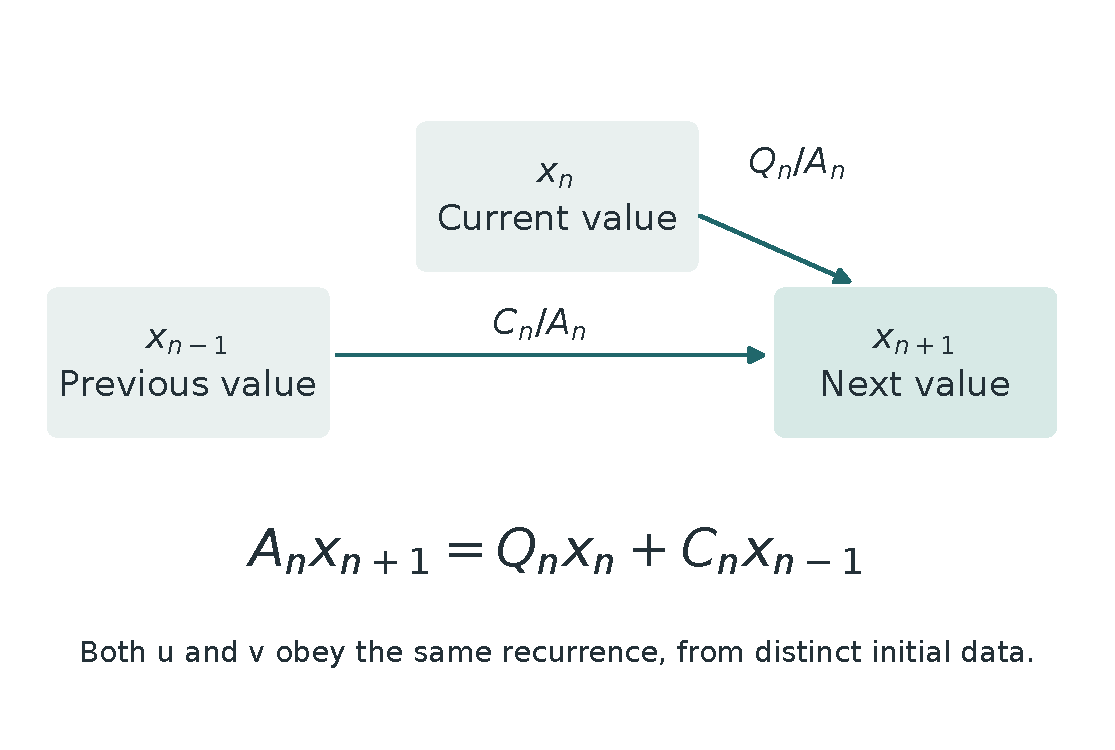
\includegraphics[width=0.93\linewidth]{../visual/figures/09_recurrence_structure.pdf}
\caption{Two preceding values determine the next rational value. The
forward rule begins at $n=1$ and uses the stated initial pair. Here and in
subsequent recurrence diagrams, $A_n=a_n$, $Q_n=q(n)$ and $C_n=c_n$.}
\label{cb_fig_recurrence}
\end{figure}

\section{Two complete forward steps}

The first steps expose all constants and signs. At $n=1$,
\[
 p(1)=13,\quad p(2)=65,\quad q(1)=10699,\qquad
 a_1=1872,\quad c_1=260.
\]
For $u$, the recurrence gives
\[
 u_2=\frac{10699(7/4)+260}{1872}
     =\frac{75933/4}{1872}=\frac{649}{64}.
\]
For $v$, its zero initial term removes the trailing contribution:
\[
 v_2=\frac{10699(13/8)+260\cdot0}{1872}
     =\frac{139087/8}{1872}=\frac{10699}{1152}.
\]
Therefore the second rational approximant is
\[
 r_2=\frac{10699}{11682}.
\]

At $n=2$ the coefficients become
\[
 p(2)=65,\quad p(3)=157,\quad q(2)=434871,\qquad
 a_2=58500,\quad c_2=22608.
\]
Using the fractions just obtained,
\begin{align*}
 u_3
 &=\frac{434871(649/64)+22608(7/4)}{58500}\\
 &=\frac{284763375/64}{58500}=\frac{19471}{256},\\[3pt]
 v_3
 &=\frac{434871(10699/1152)+22608(13/8)}{58500}\\
 &=\frac{521667445/128}{58500}=\frac{8025653}{115200}.
\end{align*}
It follows that $r_3=8025653/8761950$. All these values were also checked
against the recovered exact rational script. A floating point calculation
is unnecessary for the equality at any stage.

The first ratios are $r_0=0$ and $r_1=13/14$. The subsequent values lie
near the decimal for $G$, but proximity is only a first observation.
Chapter~\ref{cb_ch_wronskian} proves exact nested brackets and an error
sign at every index. The external identification below then makes those
brackets enclosures of Catalan's constant itself.

\section{The transfer matrix and its determinant}

Normalize the recurrence by putting
\[
 \alpha_n=\frac{q(n)}{a_n},\qquad
 \beta_n=\frac{c_n}{a_n}\qquad(n\geq1).
\]
Both quantities are positive rationals. For the adjacent state vector
$X_n(w)=(w_n,w_{n-1})^{\mathsf T}$, define
\begin{equation}\label{cb_eq_transfer}
 M_n=\begin{pmatrix}\alpha_n&\beta_n\\1&0\end{pmatrix}.
 \qquad X_{n+1}(w)=M_nX_n(w).
\end{equation}
Hence
\[
 X_{N+1}(w)=M_NM_{N-1}\cdots M_1X_1(w)\qquad(N\geq1).
\]
The order of multiplication follows the temporal order: $M_1$ acts first.
This is a product of changing matrices, not a power of one fixed matrix.

The determinant is
\[
 \det M_n=-\beta_n=-\frac{c_n}{a_n}<0.
\]
Every transfer is invertible, with
\[
 M_n^{-1}=\begin{pmatrix}0&1\\1/\beta_n&-\alpha_n/\beta_n\end{pmatrix}.
\]
An adjacent pair at index $n+1$ therefore determines the preceding pair at
index $n$, within the stated recurrence domain. This does not extend the
equation through $n=0$, where the trailing coefficient would vanish.

The two distinguished solutions can be collected into the fundamental
matrix
\[
 \mathcal F_n=
 \begin{pmatrix}u_n&v_n\\u_{n-1}&v_{n-1}\end{pmatrix},\qquad n\geq1.
\]
It satisfies $\mathcal F_{n+1}=M_n\mathcal F_n$. Its initial determinant is
\[
 \det\mathcal F_1=
 \det\begin{pmatrix}7/4&13/8\\1&0\end{pmatrix}=-\frac{13}{8}.
\]
Multiplicativity of determinants now gives
\[
 \det\mathcal F_{N+1}
 =-\frac{13}{8}\prod_{n=1}^N(-\beta_n)\ne0.
\]
Thus adjacent values of the two solutions remain independent at every
index. Each transfer reverses the determinant sign. The closed evaluation
of this product is the Wronskian theorem in
Chapter~\ref{cb_ch_wronskian}, where the factors telescope and yield exact
quotient increments. Here the matrix description identifies the mechanism
without duplicating that full proof.

\section{Continuants and the finite fraction structure}

The transfer product can also be written using continuants. For integers
$1\leq r\leq s$, let $K_{r,s}$ be the determinant of the tridiagonal matrix
whose diagonal is $\alpha_r,\ldots,\alpha_s$, lower adjacent diagonal is
one, and upper adjacent diagonal is
$-\beta_{r+1},\ldots,-\beta_s$. For instance,
\[
 K_{r,r}=\alpha_r,\qquad
 K_{r,r+1}=\det
 \begin{pmatrix}\alpha_r&-\beta_{r+1}\\1&\alpha_{r+1}\end{pmatrix}
 =\alpha_r\alpha_{r+1}+\beta_{r+1}.
\]
Set $K_{r,r-1}=1$ for the empty determinant. Expansion at the last row gives
\begin{equation}\label{cb_eq_continuant}
 K_{r,s}=\alpha_sK_{r,s-1}+\beta_sK_{r,s-2}
 \qquad(s\geq r+1).
\end{equation}
The plus sign comes from the minus sign on the upper adjacent diagonal.
This convention matches the positive trailing term in the recurrence.
All these continuants are positive rationals.

\begin{proposition}[Initial data through continuants]\label{cb_prop_continuant}
For any solution $w$ and every $n\geq2$,
\begin{equation}\label{cb_eq_continuant_solution}
 w_n=K_{1,n-1}w_1+\beta_1K_{2,n-1}w_0.
\end{equation}
\end{proposition}

\begin{proof}
At $n=2$, the formula is
$w_2=\alpha_1w_1+\beta_1w_0$, using the empty determinant for $K_{2,1}$.
At $n=3$, direct iteration gives
\[
 w_3=(\alpha_2\alpha_1+\beta_2)w_1+\alpha_2\beta_1w_0,
\]
which agrees with the formula. For later indices, both coefficients in
\eqref{cb_eq_continuant_solution} satisfy the same recurrence by
\eqref{cb_eq_continuant}. Induction finishes the proof.
\end{proof}

This expression separates the dependence on the two initial values from
the intervening recurrence coefficients. It is useful when checking a
different normalization or a shifted index: the same two continuant
coefficients must act on the corresponding initial pair.

For a positive solution, ratios of consecutive values give another finite
description. If $x_n=w_n/w_{n-1}$ is defined, then
\[
 x_{n+1}=\alpha_n+\frac{\beta_n}{x_n}.
\]
For $u$, every such ratio is defined. The first two iterations are
\[
 \frac{u_2}{u_1}=\alpha_1+\frac{\beta_1}{7/4},\qquad
 \frac{u_3}{u_2}=
 \alpha_2+\frac{\beta_2}{\alpha_1+\beta_1/(7/4)}.
\]
Repeated substitution yields a finite generalized continued fraction.
For $v$, one cannot begin with $v_1/v_0$, because $v_0=0$. Its ratio
iteration instead begins at $v_2/v_1=\alpha_1$. These formulas are exact
finite identities. Establishing a limit for an infinite continued fraction
requires an additional argument and is not implied merely by writing the
finite nested fractions.

\section{The limiting characteristic equation}

The leading terms of the coefficient polynomials are
\[
 a_n=320n^6+O(n^5),\qquad
 q(n)=3520n^6+O(n^5),\qquad
 c_n=320n^6+O(n^5).
\]
Consequently $\alpha_n\to11$, $\beta_n\to1$, and
\[
 M_n\longrightarrow M_\infty=\begin{pmatrix}11&1\\1&0\end{pmatrix}.
\]
The characteristic polynomial of this limiting matrix is
\begin{equation}\label{cb_eq_characteristic}
 \lambda^2-11\lambda-1.
\end{equation}
Its two roots are
\begin{equation}\label{cb_eq_characteristic_roots}
 \lambda_+=\frac{11+5\sqrt5}{2}=\phi^5,\qquad
 \lambda_-=\frac{11-5\sqrt5}{2}=-\phi^{-5}.
\end{equation}
Here $\phi=(1+\sqrt5)/2$. The identity $\phi^5=5\phi+3$ follows by
repeatedly using $\phi^2=\phi+1$. The roots have product $-1$, as required
by the limiting determinant, and very different magnitudes.

The limiting polynomial explains the scales that appear in the analytic
theorem, but calculating its roots is not a substitute for that theorem.
The original transfer matrices vary with $n$. One must also identify which
solution or linear combination occupies which asymptotic scale. In
particular, numerical agreement between the ratio and $G$ cannot supply
the identification of the decaying combination $u_nG-v_n$.

\begin{theorem}[External recurrence identification and rates]\label{cb_thm_source_rates}
For the exact normalization \eqref{cb_eq_uv_initial}, Zudilin's theorem and
its stated asymptotic rates give
\begin{align}
 \lim_{n\to\infty}\frac{v_n}{u_n}&=G,\label{cb_eq_source_limit}\\
 \lim_{n\to\infty}u_n^{1/n}&=\phi^5,\label{cb_eq_source_u_rate}\\
 \lim_{n\to\infty}|u_nG-v_n|^{1/n}&=\phi^{-5}.
 \label{cb_eq_source_error_rate}
\end{align}
These are external mathematical inputs, recorded precisely in source
contracts LC01 and LC02 \cite{Zudilin2003}.
\end{theorem}

The source limit is about the sequences just defined, not a differently
scaled initial pair. Multiplying both sequences by the same nonzero
constant would leave their quotient unchanged, but scaling only one
sequence would change it. The rational initial data and the source
dictionary therefore belong to the statement of the theorem.

Chapter~\ref{cb_ch_wronskian} gives a recurrence only proof that the ratios
have a limit, with strict alternating brackets. It then invokes
\eqref{cb_eq_source_limit} to name that limit $G$. This division of labor
keeps the exact recurrence reasoning visible while acknowledging the
external analytic identification.

\begin{figure}[tbp]
\centering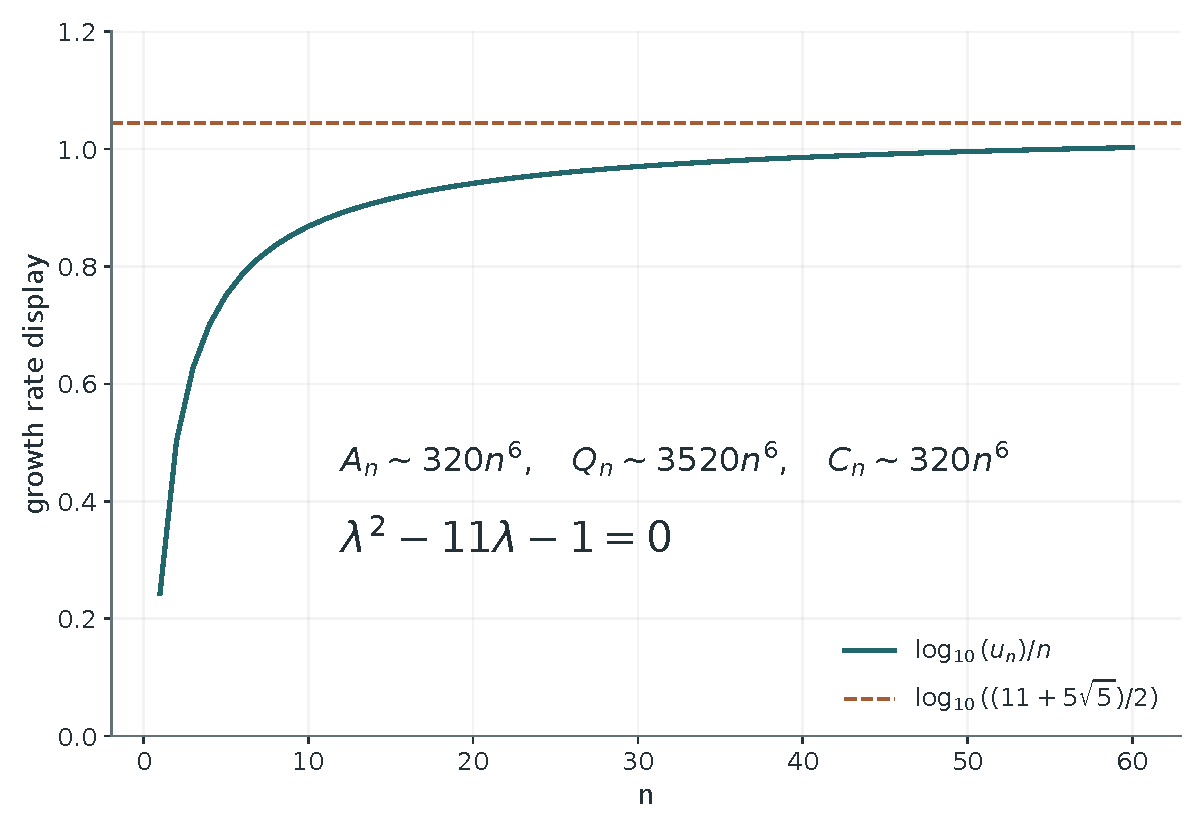
\includegraphics[width=0.92\linewidth]{../visual/figures/11_recurrence_growth.pdf}
\caption{The growing coefficient scale corresponds to the larger
characteristic root. Finite plotted values illustrate the behavior. The
universal limiting rate is a separate source theorem.}
\label{cb_fig_recurrence_growth}
\end{figure}

\section{Normalized error and the arithmetic question}

An immediate consequence of the two source rates is
\begin{equation}\label{cb_eq_ratio_error_rate}
 \lim_{n\to\infty}|G-r_n|^{1/n}
 =\lim_{n\to\infty}\frac{|u_nG-v_n|^{1/n}}{u_n^{1/n}}
 =\phi^{-10}.
\end{equation}
Thus the ratio error has a smaller exponential scale than the unnormalized
linear form. The distinction comes from division by the growing
coefficient $u_n$. Also, since $r_n\to G>0$, one has
$r_n^{1/n}\to1$ and consequently $v_n^{1/n}\to\phi^5$. Both individual
sequences grow, while their specified linear combination decays.

The scaled coefficient used in the packet construction has rate
\[
 \lim_{n\to\infty}(16^nu_n)^{1/n}
 =16\phi^5=88+40\sqrt5.
\]
Chapter~\ref{cb_ch_integrality} proves that this scaled coefficient is an
integer at every index using a separate half binomial identity. Its growth
rate and its integrality are distinct mathematical facts.

\begin{figure}[tbp]
\centering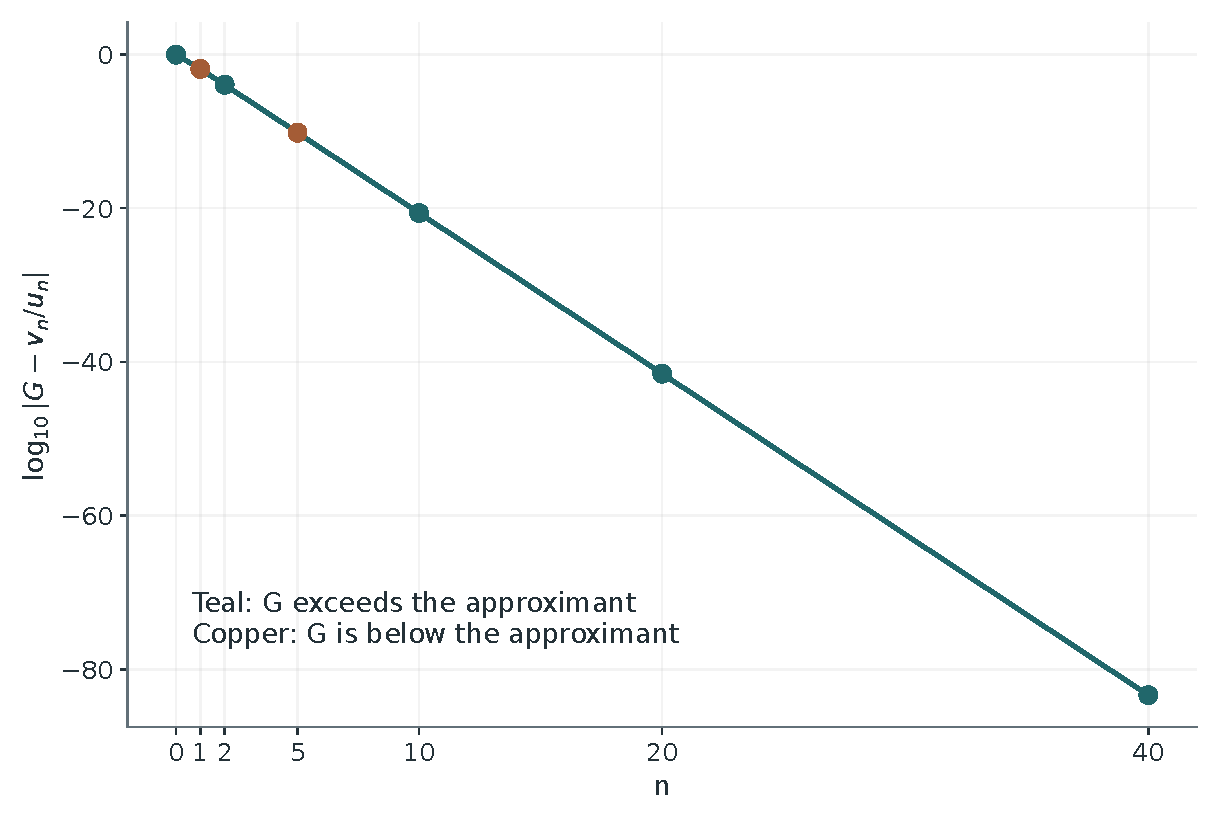
\includegraphics[width=0.92\linewidth]{../visual/figures/12_approximant_error.pdf}
\caption{The normalized rational error decreases rapidly. Exact interval
computations support the finite plotted values. The asymptotic rate
depends on the identified source solution, and irrationality requires
denominator control in addition.}\label{cb_fig_ratio_error}
\end{figure}

The approximants therefore do much more than the original alternating
partial sums in numerical accuracy. Their rapid convergence still does
not classify the limit as irrational. The fractions $u_n$ and $v_n$ carry
denominators, and the denominator of their ratio may grow rapidly too.
To apply the integer lattice criterion, one must turn the error into a
nonzero integer linear form and show that its size tends to zero after
all necessary clearing. The recurrence supplies the coefficients and the
analytic theorem supplies the error scale. The subsequent determinant,
integrality and packet chapters examine the additional arithmetic needed
to connect these facts to that criterion.

\chapter{The determinant that controls the approximants}
\label{cb_ch_wronskian}

The recurrence produces two rational sequences. Its most useful internal
certificate is the determinant of two adjacent coefficient pairs. This
determinant can be evaluated without knowing Catalan's constant, without a
decimal approximation to it, and without any assumption about its arithmetic
nature. It proves that the two sequences remain independent and gives an
exact description of the movement of their quotient.

\section{A determinant with a closed formula}

Write the recurrence in the form
\begin{equation}\label{cb_eq_rec_short}
 a_n w_{n+1}=q(n)w_n+c_nw_{n-1},\qquad n\geq1,
\end{equation}
where, in this chapter only,
\[
 a_n=(2n+1)^2(2n+2)^2p(n),\qquad
 c_n=(2n-1)^2(2n)^2p(n+1).
\]
These are recurrence coefficients, not the integer coefficients of a cleared
linear form used later. In particular, both are positive. The initial data are
\[
 u_0=1,\quad u_1=\frac74,\qquad
 v_0=0,\quad v_1=\frac{13}{8}.
\]
The polynomial $p(n)=20n^2-8n+1$ is positive for integer $n\geq0$.
Define the discrete Wronskian
\begin{equation}\label{cb_eq_W_def}
 W_n=u_{n+1}v_n-u_nv_{n+1},\qquad n\geq0.
\end{equation}
This convention fixes its sign. Reversing the two terms reverses every sign
in the subsequent formulas.

\begin{theorem}[Exact Wronskian]\label{cb_thm_W}
For every integer $n\geq0$,
\begin{equation}\label{cb_eq_W_closed}
 W_n=\frac{(-1)^{n+1}p(n+1)}{2(2n+1)^2(2n+2)^2}.
\end{equation}
In particular, $W_n\ne0$.
\end{theorem}

\begin{proof}
At $n=0$ the determinant is $-13/8$, which agrees with the displayed
formula because $p(1)=13$. For $n\geq1$, insert
\eqref{cb_eq_rec_short} into both terms of \eqref{cb_eq_W_def}. The terms
containing $q(n)u_nv_n$ cancel, leaving
\[
 W_n=\frac{c_n}{a_n}(u_{n-1}v_n-u_nv_{n-1})
     =-\frac{c_n}{a_n}W_{n-1}.
\]
Iterating this equality gives
\[
 W_n=(-1)^nW_0
 \prod_{j=1}^n
 \frac{(2j-1)^2(2j)^2p(j+1)}{(2j+1)^2(2j+2)^2p(j)}.
\]
There are two independent telescopes. The polynomial factors leave
$p(n+1)/p(1)$. The integer factors leave
$4/((2n+1)^2(2n+2)^2)$. Substituting $W_0=-13/8$ and $p(1)=13$
proves the identity. The empty product gives the same calculation at $n=0$.
\end{proof}

The proof is universal. A rational arithmetic check of its first 201
instances is an implementation check, not its logical foundation. The finite
check is still useful because it can detect a shifted index or a reversed
determinant convention. The first values make those conventions visible.

\begin{center}
\begin{tabular}{@{}rrrrr@{}}
\toprule
$n$ & $0$ & $1$ & $2$ & $3$\\
\midrule
$W_n$ & $-13/8$ & $65/288$ & $-157/1800$ & $289/6272$\\
\bottomrule
\end{tabular}
\end{center}

\begin{figure}[tbp]
\centering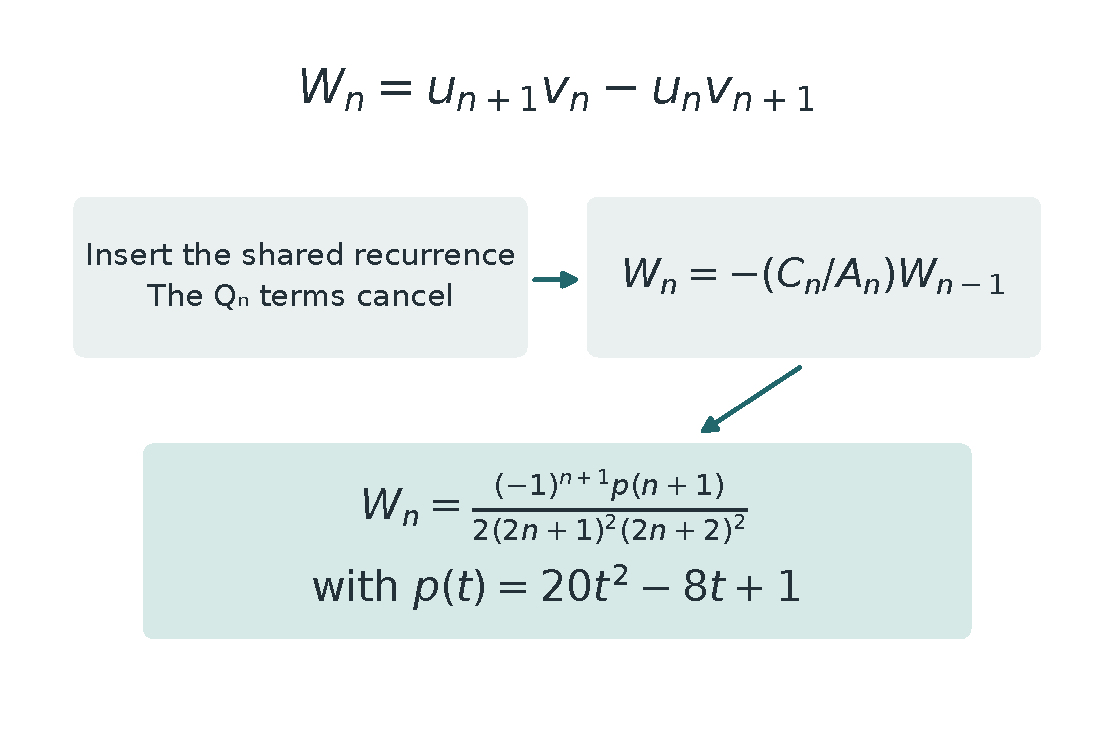
\includegraphics[width=0.92\linewidth]{../visual/figures/14_wronskian_identity.pdf}
\caption{The determinant recurrence loses the middle coefficient. Its
remaining product telescopes exactly. The figure illustrates the written
identity, which holds at every index.}\label{cb_fig_W_identity}
\end{figure}

\section{Positive coefficients and decreasing steps}

The next argument needs the positivity of $u_n$. It also needs a modest lower
bound on it, rather than a full asymptotic theorem. Both follow from the
recurrence. To see the relevant sign without relying on a plot, put $t=n-1$.
Direct polynomial expansion gives
\begin{align*}
 q(n)-a_n={}&3200t^6+24000t^5+73392t^4+117072t^3\\
            &+102768t^2+47112t+8827.
\end{align*}
Thus $q(n)>a_n>0$ for every $n\geq1$. Starting from $u_1>u_0>0$, the
recurrence implies
\[
 u_{n+1}>\frac{q(n)}{a_n}u_n>u_n.
\]
In particular $u_n\geq1$. This elementary bound is enough for the convergence
argument below.

Set
\begin{equation}\label{cb_eq_ratio_steps}
 r_n=\frac{v_n}{u_n},\qquad
 d_n=\frac{p(n+1)}{2(2n+1)^2(2n+2)^2u_nu_{n+1}}.
\end{equation}
The symbol $d_n$ denotes a positive rational step size. It is unrelated to
the least common multiples $L_N$ used in denominator clearing. Dividing the
Wronskian identity by $u_nu_{n+1}$ yields
\begin{equation}\label{cb_eq_alternating_steps}
 r_{n+1}-r_n=(-1)^n d_n.
\end{equation}
The movement of the approximants therefore alternates exactly.

\begin{lemma}[Strict decrease of the step sizes]\label{cb_lem_d_decrease}
The rational numbers $d_n$ are strictly positive, decrease strictly, and tend
to zero.
\end{lemma}

\begin{proof}
Positivity is immediate. For $n\geq1$, the determinant recurrence gives
\[
 \frac{d_n}{d_{n-1}}
 =\frac{c_n}{a_n}\frac{u_{n-1}}{u_{n+1}}<1.
\]
The strict inequality follows from
$a_nu_{n+1}=q(n)u_n+c_nu_{n-1}>c_nu_{n-1}$.
Finally $u_nu_{n+1}\geq1$, so
\[
 0<d_n\leq
 \frac{p(n+1)}{2(2n+1)^2(2n+2)^2}\longrightarrow0.
\]
No limiting characteristic root is needed for this conclusion.
\end{proof}

This is a useful example of the distinction between two arguments with
different jobs. The exponential rates from Zudilin's theorem describe the
quality of large approximants. The simple inequalities above establish
convergence and strict brackets directly from rational recurrence data.

\section{The limit and its exact rational brackets}

\begin{theorem}[Alternating brackets]\label{cb_thm_brackets}
There is a real number $L$ such that $r_n\to L$. For every $k\geq0$,
\begin{equation}\label{cb_eq_bracket}
 r_{2k}<L<r_{2k+1}.
\end{equation}
The even subsequence increases strictly and the odd subsequence decreases
strictly. For every $n\geq0$,
\begin{equation}\label{cb_eq_error_bounds}
 d_n-d_{n+1}<|L-r_n|<d_n,
 \qquad \operatorname{sign}(L-r_n)=(-1)^n.
\end{equation}
\end{theorem}

\begin{proof}
Equation \eqref{cb_eq_alternating_steps} and the preceding lemma identify
$r_n$ with partial sums of a convergent alternating series:
\[
 r_n=\sum_{j=0}^{n-1}(-1)^j d_j,
 \qquad L=\sum_{j=0}^{\infty}(-1)^j d_j.
\]
For the even subsequence,
$r_{2k+2}-r_{2k}=d_{2k}-d_{2k+1}>0$.
For the odd subsequence,
$r_{2k+3}-r_{2k+1}=-d_{2k+1}+d_{2k+2}<0$.
Their adjacent separation $d_{2k}$ tends to zero, so they have the same limit.
Strictness of both subsequences places that limit strictly between every
displayed pair. The alternating tail beginning with $d_n$ gives the sign
and upper bound in \eqref{cb_eq_error_bounds}. Pairing its first two terms
and then successive pairs gives the strict lower bound. All omitted pairs
are positive after multiplication by $(-1)^n$.
\end{proof}

The endpoints in \eqref{cb_eq_bracket} are exact rationals. For example,
the first few approximants are
\begin{center}
\begin{tabular}{@{}rl@{}}
\toprule
$n$ & $r_n$\\
\midrule
$0$ & $0$\\
$1$ & $13/14$\\
$2$ & $10699/11682$\\
$3$ & $8025653/8761950$\\
\bottomrule
\end{tabular}
\end{center}
There is no rounding decision in these brackets. Increasing the index
nests a narrower interval inside the earlier one. A program can use the
same determinant to check the interval width exactly.

The recurrence and its initial values establish a limit $L$. The statement
that this limit is $G$ is a separate mathematical identification. We use
Zudilin's Theorem 1 for that identification, with the normalization recorded
in source contract LC01 \cite{Zudilin2003}. After this external input,
\eqref{cb_eq_bracket} and \eqref{cb_eq_error_bounds} become exact bounds for
Catalan's constant and its rational approximants. In particular,
\begin{equation}\label{cb_eq_linear_error_sign}
 (-1)^n(u_nG-v_n)>0\qquad(n\geq0).
\end{equation}

This order of reasoning prevents a circular shortcut. Decimal agreement
between $r_n$ and a familiar constant does not identify a limit. Nor does
the nonzero Wronskian alone exclude equality between one particular
approximant and an arbitrary real number. The strict brackets supply
nonvanishing for the recurrence limit, and the source theorem then identifies
that limit with $G$.

\section{What this certificate does and does not settle}

The determinant settles several questions completely. Adjacent coefficient
pairs never become proportional. The ratio has a unique limit. Its even and
odd approximants bracket that limit, and their signs of error are fixed.
Each of these conclusions has a written argument valid at every index.

The determinant does not classify the limit as rational or irrational. A
sequence of distinct rational numbers with alternating errors can converge
to a rational number. Irrationality requires an additional comparison
between error size and the integer lattice after clearing denominators.
The Wronskian contributes exact nonvanishing and useful quantitative bounds,
but it does not pay the arithmetic cost of that clearing. The next chapters
keep these two requirements visible in the same coefficient construction.

\chapter{Integer coefficients and the corrected integral}
\label{cb_ch_integrality}

The rational recurrence is an efficient way to construct coefficients. It
does not by itself explain their denominators. A second description, in
terms of half integer binomial coefficients, gives a short universal
integrality proof. A third description, as a positive integral, supplies the
analytic error. Matching these descriptions requires care with constants.
In the source used here, one printed integral factor fails even at the
initial index. We record that failure and derive the factor used throughout
this edition.

\section{A coefficient identity, rather than an irrationality assumption}

Krattenthaler and Rivoal use coefficients $a_n,b_n$ for a linear form in
Catalan's constant \cite{KR2008}. These letters belong to their source and
do not denote the recurrence coefficients of the previous chapter. In the
normalization of this book their coefficients satisfy
\begin{equation}\label{cb_eq_KR_dictionary}
 a_n=-4u_n,\qquad b_n=-4v_n.
\end{equation}
The notation bridge is recorded in source contract LC05. After shifting the
source summation variable by one, their hypergeometric series is $-1/2$
times Zudilin's series. The source partial fraction expansion identifies
the two rational coefficients separately, giving
\eqref{cb_eq_KR_dictionary}.

It would be invalid to obtain this dictionary merely by equating two real
expressions in $G$ and then treating $1$ and $G$ as linearly independent over
$\Q$. That independence is exactly the irrationality under investigation.
Instead, take a formal variable $X$. The partial fraction coefficient
calculation identifies the polynomial $a_nX-b_n$ with
$-4(u_nX-v_n)$ in $\Q[X]$. Equality of coefficients in a polynomial ring
does not depend on the arithmetic nature of any later substitution for
$X$. This distinction also applies to the packet coefficients below.

The same source gives the explicit finite sum
\begin{equation}\label{cb_eq_halfbinomial}
 u_n=\sum_{j=0}^n
 \binom nj\binom{n-\tfrac12}{j}\binom{n+j-\tfrac12}{j},\qquad n\geq0.
\end{equation}
Here
\[
 \binom{x}{0}=1,\qquad
 \binom{x}{j}=\frac{x(x-1)\cdots(x-j+1)}{j!}\quad(j\geq1)
\]
defines the generalized binomial coefficient. Formula
\eqref{cb_eq_halfbinomial} is Lemma 3, equation (3.1), after the coefficient
normalization above. Its identification with the recurrence is an external
source input. The denominator argument that follows is elementary and is
written in full.

\section{The exact integer sequence}

Define
\begin{equation}\label{cb_eq_T_def}
 T_n=16^nu_n.
\end{equation}
The importance of the power $16^n$ is that it clears each summand of
\eqref{cb_eq_halfbinomial}, rather than relying on cancellation between
different summands.

\begin{lemma}[Half binomial denominators]\label{cb_lem_half_denom}
For integers $h,j\geq0$, the number
$4^j\binom{h-\tfrac12}{j}$ is an integer.
\end{lemma}

\begin{proof}
Work with formal power series, so no convergence issue arises. The central
binomial expansion gives
\[
 (1+4z)^{-1/2}=\sum_{k\geq0}(-1)^k\binom{2k}{k}z^k.
\]
Every coefficient is an integer. Multiplying by the integer polynomial
$(1+4z)^h$ preserves this property. The coefficient of $z^j$ in the product
is $4^j\binom{h-\tfrac12}{j}$. More explicitly it is
\[
 \sum_{\ell=0}^{\min(h,j)}
 \binom h\ell 4^\ell(-1)^{j-\ell}
 \binom{2(j-\ell)}{j-\ell},
\]
an integer sum.
\end{proof}

\begin{theorem}[Universal integrality of $T_n$]\label{cb_thm_T_integer}
For every integer $n\geq0$, $T_n$ is a positive integer. In fact, after
multiplication by $16^n$, each summand in
\eqref{cb_eq_halfbinomial} is an integer.
\end{theorem}

\begin{proof}
For $0\leq j\leq n$, apply the preceding lemma with $h=n$ and $h=n+j$.
The scaled summand is
\[
 16^{n-j}\binom nj
 \left(4^j\binom{n-\tfrac12}{j}\right)
 \left(4^j\binom{n+j-\tfrac12}{j}\right).
\]
All four factors are integers. Summing proves integrality. Every original
summand is positive: the generalized binomial factors have only positive
factors in their defining products when $j\leq n$. The $j=0$ term is one,
including at $n=0$. Thus the sum is positive.
\end{proof}

For example, the $n=2$ sum is
\[
 u_2=1+\frac{15}{2}+\frac{105}{64}=\frac{649}{64}.
\]
Multiplication by $16^2$ gives the three integers $256$, $1920$, and $420$,
whose sum is $T_2=2596$. This illustrates the proof at the level of individual
terms. The first sequence values are
\[
 T_0=1,\quad T_1=28,\quad T_2=2596,\quad
 T_3=311536,\quad T_4=41759524.
\]

The source theorem $16^na_n\in\Z$, combined with
\eqref{cb_eq_KR_dictionary}, would establish only $4T_n\in\Z$ directly.
Division by four is not an integrality argument. The half binomial proof
above establishes the stronger statement actually needed by the integer
packet construction. It removes a possible hidden dependence on a finite
exact division experiment.

The recurrence for $T_n$ is obtained by multiplying the original recurrence
by $16^{n+1}$:
\begin{equation}\label{cb_eq_T_recurrence}
 a_nT_{n+1}=16q(n)T_n+256c_nT_{n-1}\qquad(n\geq1).
\end{equation}
A program can therefore generate $T_n$ using integer numerators and exact
division by $a_n$. A nonzero remainder is a failed implementation check and
must terminate the computation. The written theorem establishes why exact
division succeeds universally for the correctly normalized recurrence.

\begin{figure}[tbp]
\centering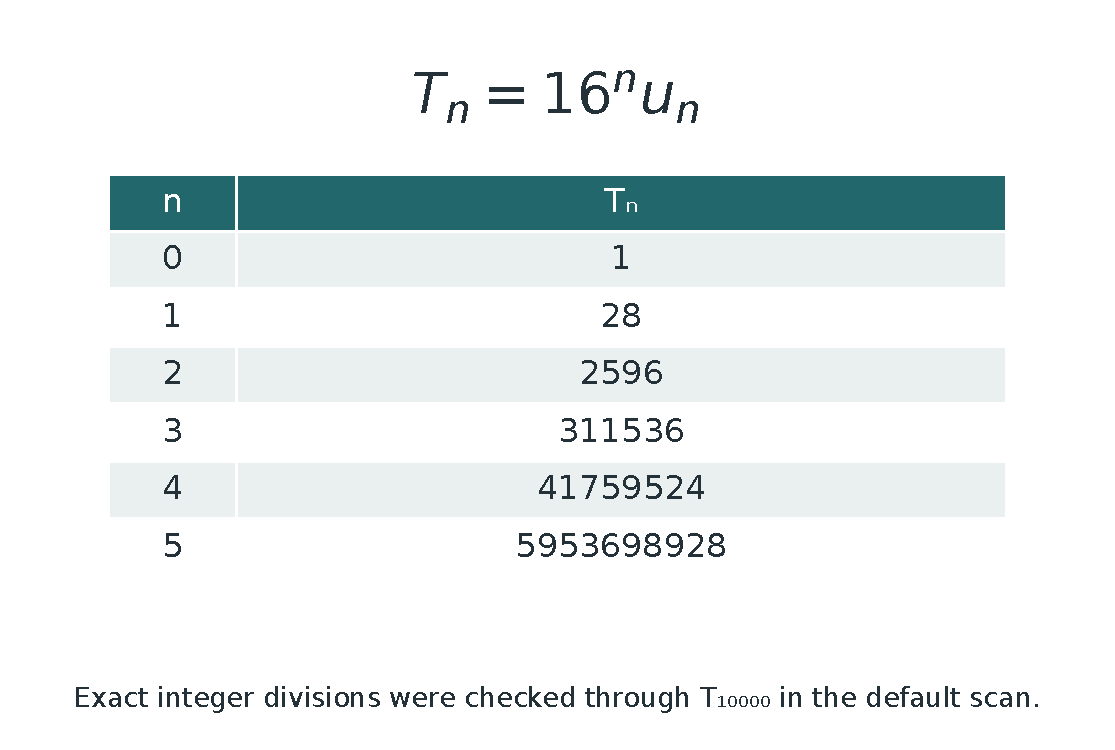
\includegraphics[width=0.93\linewidth]{../visual/figures/15_scaled_coefficients.pdf}
\caption{The recurrence coefficients become an integer sequence after
scaling by $16^n$. The finite values shown here accompany a universal
half binomial denominator proof.}\label{cb_fig_T}
\end{figure}

\section{The rational coefficient has a different clearing cost}

Put
\[
 L_N=\operatorname{lcm}(1,2,\ldots,N),\qquad L_0=1.
\]
The source's least common multiple notation is translated to $L_N$ here.
The letter $D$ will later denote an actual reduced denominator, which can
be much smaller than this universal clearing bound.
Krattenthaler and Rivoal's Theorem 2 gives
$16^nL_{2n}^2b_n\in\Z$ for positive integer $n$
\cite{KR2008}. In the present normalization it implies
\begin{equation}\label{cb_eq_v_sharp_clear}
 4\cdot16^nL_{2n}^2v_n\in\Z\qquad(n\geq0).
\end{equation}
The case $n=0$ is immediate from $v_0=0$. In particular the historical
script's weaker clearing factor, with $8$ in place of $4$, is valid at every
index. This is a source theorem about the rational coefficient. The
half binomial argument for $u_n$ does not automatically prove it.

Earlier asymptotic denominator bounds in Zudilin's remarks establish the
appropriate exponential scale with a logarithmic correction in the exponent
\cite{Zudilin2002}. They serve a different purpose from exact clearing at
every index. An asymptotic expression involving $o(n)$ should not be read
as a precise power of two that can be inserted into a finite computation.
For the packet arithmetic we use \eqref{cb_eq_v_sharp_clear} and the exact
integer theorem for $T_n$.

The finite direct product check in this release compares
\eqref{cb_eq_halfbinomial} with a separately indexed rational recurrence for
every $n=0,\ldots,50$. It checks 1326 summands, including the two half
binomial denominator statements and scaled integrality of each term. The
independent recurrence check extends through $n=500$ and verifies the weaker
factor $8$ clearing there. These are useful finite corroborations. The
external identity and the two universal arithmetic arguments have their
own evidence and remain distinct from those checks.

\section{A printed factor that fails at the initial index}

Consider the positive double integral
\begin{equation}\label{cb_eq_J_def}
 J_n=\int_0^1\!\int_0^1
 \frac{x^{n-1/2}(1-x)^ny^n(1-y)^{n-1/2}}
 {(1-xy)^{n+1}}\,\dd x\,\dd y,
 \qquad n\geq0.
\end{equation}
Zudilin's Theorem 3 prints $u_nG-v_n=(-1)^nJ_n/4$ in both the authenticated
arXiv version and the published journal PDF \cite{Zudilin2003}. With
$u_0=1$ and $v_0=0$, this would force $J_0=4G$.
The integral itself gives $J_0=8G$. Thus that printed factor cannot be used
with these initial conditions. This edition uses
\begin{equation}\label{cb_eq_J_correct}
 J_n=8(-1)^n(u_nG-v_n).
\end{equation}
No erratum was recovered in the bounded source search. The correction is
supported by the explicit derivation below, rather than an assertion that
a published correction exists.

The initial integral supplies a short diagnostic. Substitute $x=t^2$ and
$y=1-s^2$. Then
\begin{align*}
 J_0
 &=4\int_0^1\!\int_0^1\frac{\dd s\,\dd t}{1-t^2+t^2s^2}\\
 &=4\int_0^1\frac{\arcsin t}{t\sqrt{1-t^2}}\,\dd t
  =4\int_0^{\pi/2}\theta\csc\theta\,\dd\theta.
\end{align*}
Since an antiderivative of $\csc\theta$ is $\log\tan(\theta/2)$, integration
by parts yields
\[
 J_0=-4\int_0^{\pi/2}\log\tan(\theta/2)\,\dd\theta
     =-8\int_0^{\pi/4}\log\tan z\,\dd z=8G.
\]
Both boundary terms vanish. At zero this uses
$\theta\log\tan(\theta/2)\to0$, and at $\pi/2$ the logarithm is zero.

Checking one index detects the wrong normalization. It does not by itself
prove \eqref{cb_eq_J_correct} for every $n$. The next calculation explains
the all index extension and identifies its external transformation input.

\section{The all index normalization}

Expanding $(1-xy)^{-n-1}$ as its nonnegative binomial series and applying
Tonelli's theorem gives
\begin{equation}\label{cb_eq_beta_H}
 J_n=C_nH_n,
\end{equation}
where
\[
 C_n=\frac{\Gamma(n+1)^2\Gamma(n+\tfrac12)^2}
 {\Gamma(2n+\tfrac32)^2},
\]
and
\[
 H_n={}_3F_2\!\left(
 \begin{matrix}n+1,n+\tfrac12,n+1\\
 2n+\tfrac32,2n+\tfrac32\end{matrix};1\right).
\]
Indeed, the two beta integrals in the term with index $k$ are
$B(n+\tfrac12+k,n+1)$ and $B(n+1+k,n+\tfrac12)$.
Their ratios to the corresponding $k=0$ integrals give exactly the displayed
hypergeometric parameters. The excess of the lower parameters over the
upper parameters is $n+1/2>0$, so the series converges for every $n\geq0$.

Let $E_n$ denote the well poised ${}_6F_5$ series at $-1$ in Zudilin's
displayed Whipple transformation, with
$a=3n+1$, $b=c=d=n+1/2$, and $e=n+1$. The transformation states
\[
 H_n=\frac{\Gamma(3n+2)\Gamma(n+\tfrac12)}
 {\Gamma(2n+\tfrac32)\Gamma(2n+1)}E_n.
\]
Its condition $\operatorname{Re}(1+a-d-e)>0$ becomes $n+1/2>0$ here.
The displayed prefactor of the source hypergeometric form $F_n^{\rm src}$
is
\[
 F_n^{\rm src}=(-1)^n
 \frac{\Gamma(n+1)^2\Gamma(3n+2)\Gamma(n+\tfrac12)^3}
 {\Gamma(2n+\tfrac32)^3\Gamma(2n+1)}E_n.
\]
Substitution in \eqref{cb_eq_beta_H} therefore gives
$F_n^{\rm src}=(-1)^nJ_n$. There is no additional factor two in the gamma
cancellation. The formal partial fraction coefficient identification in
the same source gives $F_n^{\rm src}=8(u_nG-v_n)$, with the recurrence
initial data used here. Combining these two identities proves
\eqref{cb_eq_J_correct} at every index.

The beta integral expansion and prefactor cancellation are written
calculations. The Whipple transformation and the partial fraction
identification are external mathematical inputs from the authenticated
paper. Their precise roles are recorded in LC03 and the accompanying
normalization audit. The independent initial integral agrees with the
result, and Eskandari's coefficient normalization uses the same factor $8$
\cite{Eskandari2026}.

\section{Three descriptions, three different guarantees}

The recurrence permits efficient exact computation. The half binomial
formula proves that $16^nu_n$ is always an integer. The integral describes
the error and makes its sign transparent after the corrected normalization.
These descriptions agree, but each answers a different question. Keeping
their roles distinct prevents a finite arithmetic check from being mistaken
for an analytic theorem, or a positive integral from being mistaken for
denominator control. The packet construction will use all three.

\chapter{The binomial packet and the integral filter}
\label{cb_ch_packets}

The packet combines a finite block of recurrence coefficients. Its integer
part is a positive binomial sum, while its error part is a signed integral.
These two facts coexist because the signs in the original error already
alternate. The packet removes those coefficient signs and replaces them
with a polynomial filter inside the integral. That filter is useful for
approximation, but its changing sign imposes a real restriction on any
nonvanishing argument.

\section{A finite transform with an exact additive evolution}

For integers $n,m\geq0$, define
\begin{align}
 S_{n,m}&=\sum_{i=0}^m\binom miT_{n+i},\label{cb_eq_S_def}\\
 H_{n,m}&=\sum_{i=0}^m\binom mi16^{n+i}v_{n+i}.
 \label{cb_eq_H_packet_def}
\end{align}
The two index symbol $H_{n,m}$ denotes a rational packet coefficient. It is
distinct from the hypergeometric function $H_n$ used in the integral
normalization derivation. The theorem on $T_n$ proves
$S_{n,m}\in\Z_{>0}$ at every pair. The coefficient $H_{n,m}$ is rational
and requires separate denominator clearing.

\begin{proposition}[Pascal evolution]\label{cb_prop_Pascal}
For $n,m\geq0$,
\begin{equation}\label{cb_eq_Pascal}
 S_{n,m+1}=S_{n,m}+S_{n+1,m}.
\end{equation}
The same identity holds with $H$ in place of $S$.
\end{proposition}

\begin{proof}
Use $\binom{m+1}{i}=\binom mi+\binom m{i-1}$, with out of range binomial
coefficients interpreted as zero. The first contribution is $S_{n,m}$.
Changing $i$ to $i+1$ in the second contribution gives $S_{n+1,m}$. The
argument uses only the finite weights, so it applies to either seed
sequence.
\end{proof}

At $m=0$, the packet is just $S_{n,0}=T_n$. The first two nontrivial rows
are
\[
 S_{n,1}=T_n+T_{n+1},\qquad
 S_{n,2}=T_n+2T_{n+1}+T_{n+2}.
\]
For example $S_{1,1}=28+2596=2624$. The Pascal identity produces exactly
the same integer as direct evaluation of its defining sum. This agreement
between an additive row evolution and a direct weighted sum gives two
different implementations of the finite transform.

If $E$ denotes the shift operator $(Ef)_n=f_{n+1}$, the packet is
$(1+E)^mT$ at index $n$. This is an identity about a finite polynomial in
one shift. It does not introduce a further assumption about recurrence
solutions or convergence. Reduction modulo a power of two commutes with
this polynomial, which is the basis of the valuation computation in the
next chapter.

\begin{figure}[tbp]
\centering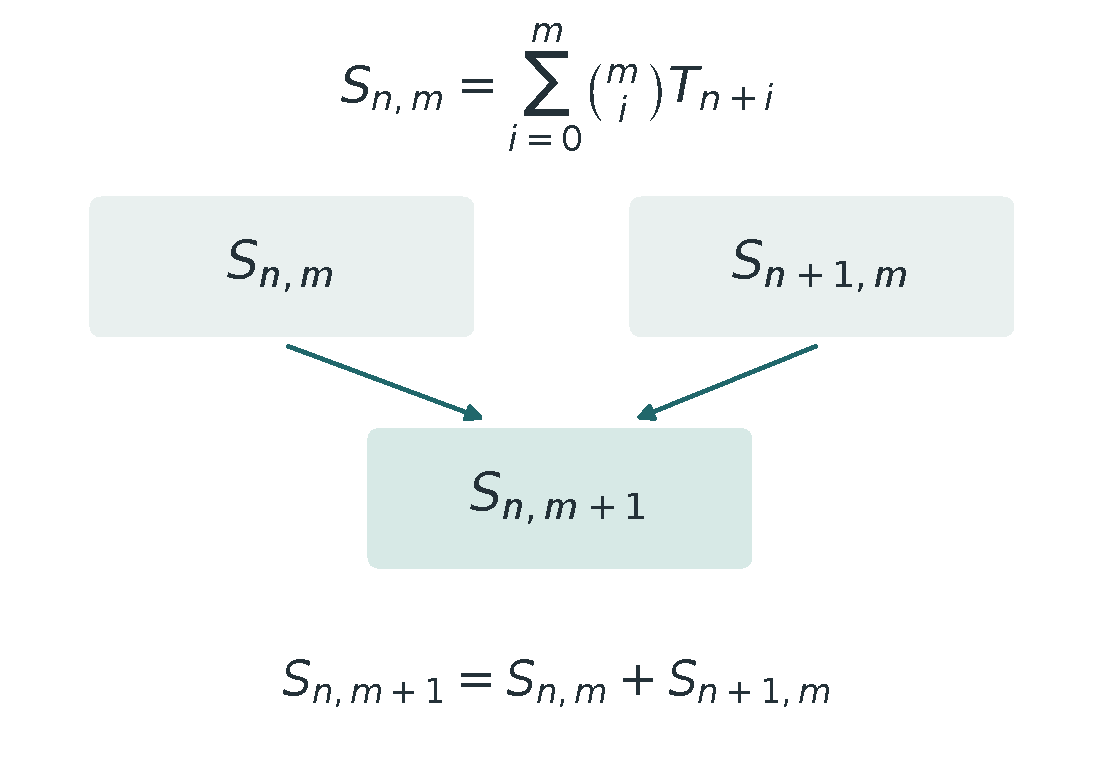
\includegraphics[width=0.91\linewidth]{../visual/figures/16_pascal_transform.pdf}
\caption{Each new packet row is the sum of adjacent entries in the
preceding row. This exact identity is also valid after modular reduction.}
\label{cb_fig_Pascal}
\end{figure}

\section{The source filter and the raw form}

Eskandari's preprint applies the filter
\begin{equation}\label{cb_eq_Jtilde}
 \widetilde J_{n,m}=\sum_{i=0}^m(-16)^i\binom miJ_{n+i}
 \qquad(n,m\geq0)
\end{equation}
to the integral family \cite{Eskandari2026}. The filter and its approximation
analysis are external work. This book examines its coefficient arithmetic
and the finite evidence recovered from the project's script.

Substitute the corrected normalization
$J_k=8(-1)^k(u_kG-v_k)$ into \eqref{cb_eq_Jtilde}. The two factors
$(-1)^i$ cancel. Thus
\begin{equation}\label{cb_eq_Jtilde_coeffs}
 \widetilde J_{n,m}=8(-1)^n16^{-n}(S_{n,m}G-H_{n,m}).
\end{equation}
Define the raw packet form
\begin{equation}\label{cb_eq_raw_F}
 F_{n,m}=16^n\widetilde J_{n,m}
        =8(-1)^n(S_{n,m}G-H_{n,m}).
\end{equation}
The adjective raw means that the common denominator of $H_{n,m}$ has not
yet been cleared. It does not mean that $F_{n,m}$ is an integer linear form.
The coefficient of $G$ is an integer, but the other coefficient may be
rational.

This normalization is important for comparison with historical data.
Multiplying or dividing a linear form by a growing power changes its
displayed decay rate. The integral filter is $\widetilde J_{n,m}$, while
the recorded arithmetic form $F_{n,m}$ is $16^n$ times it. Their signs and
zeros agree because $16^n>0$. Their logarithmic size per unit $n$ differs by
$\log16$.

\section{The measure and its sign changing polynomial}

On the open unit square, set
\begin{equation}\label{cb_eq_psi_mu}
 \psi(x,y)=\frac{xy(1-x)(1-y)}{1-xy},\qquad
 \dd\mu=\frac{\dd x\,\dd y}{\sqrt{x(1-y)}(1-xy)}.
\end{equation}
The factor $1-xy$ is outside the square root. Moving that factor inside, as in
\[
 \frac{\dd x\,\dd y}{\sqrt{x(1-y)(1-xy)}},
\]
would represent a different integral. With the measure in \eqref{cb_eq_psi_mu},
\[
 J_n=\int_{(0,1)^2}\psi^n\,\dd\mu,
 \qquad
 \widetilde J_{n,m}=\int_{(0,1)^2}\psi^n(1-16\psi)^m\,\dd\mu.
\]
The second identity follows by the ordinary binomial theorem inside a
finite sum. The total measure is $J_0=8G<\infty$.

The kernel has a simple maximum that also explains why the filter changes
sign. Put $r=\sqrt{xy}$. Since $x+y\geq2r$,
\[
 \psi(x,y)\leq\frac{r^2(1-r)^2}{1-r^2}
              =\frac{r^2(1-r)}{1+r},\qquad0<r<1.
\]
Equality is achieved when $x=y=r$. The derivative of the last expression
is
\[
 \frac{2r(1-r-r^2)}{(1+r)^2}.
\]
It has its interior maximum at $r=\phi^{-1}$, where
$\phi=(1+\sqrt5)/2$. Since $1-r=r^2$ there, the maximum is
\begin{equation}\label{cb_eq_psi_max}
 \max\psi=\phi^{-5}\approx0.09017.
\end{equation}
This is greater than $1/16$. One can already see a negative filter value
at $x=y=1/2$, where $\psi=1/12$ and $1-16\psi=-1/3$.
Near the sides of the square $\psi$ is small and the filter is positive.

\begin{theorem}[Nonvanishing for even filter order]\label{cb_thm_even_positive}
For every $n\geq0$ and every even integer $m\geq0$,
$\widetilde J_{n,m}>0$ and $F_{n,m}>0$.
\end{theorem}

\begin{proof}
For even $m$, the integrand $\psi^n(1-16\psi)^m$ is nonnegative. It is
strictly positive on an open subset of the square with $0<\psi<1/16$.
The measure has positive density there. Hence its integral is strictly
positive. It is finite because $\psi$ and $1-16\psi$ are bounded and
$\mu$ has finite total mass. Multiplication by $16^n$ preserves positivity.
\end{proof}

This theorem includes $m=0$ and $n=0$. It does not require that $G$ be
irrational. Indeed, positivity is one of the ingredients that an eventual
irrationality criterion would combine with sufficiently small cleared
integer forms. The even order restriction is easy to impose along an
asymptotic slope by choosing $m(n)$ to be the nearest suitable even integer.
The change in $m/n$ then tends to zero.

\section{The odd sign hypothesis failed}

For odd $m$, the polynomial factor changes sign, so the preceding positivity
proof does not apply. A proposed shortcut was the sign pattern
$\operatorname{sign}F_{n,m}=(-1)^m$. The finite audit falsified it. The first
counterexample is the pair $(n,m)=(1,1)$.

Using $u_1=7/4$, $v_1=13/8$, $u_2=649/64$ and $v_2=10699/1152$, one obtains
\[
 S_{1,1}=2624,\qquad H_{1,1}=\frac{21632}{9}.
\]
Consequently
\begin{equation}\label{cb_eq_odd_counterexample}
 F_{1,1}=\frac{173056}{9}-20992G>0.
\end{equation}
The inequality is certified by the exact rational enclosure of $G$ recorded
in the independent computation. The threshold for it is $G<338/369$.
The enclosure lies strictly below that rational number. Thus this form is
positive although $m$ is odd, contradicting the proposed pattern.
The sign is decided by rational interval endpoints, rather than floating
point subtraction between nearly equal numbers.

The audit checks 860 pairs with $1\leq n\leq20$ and $0\leq m\leq4n$.
Every tested form is certified nonzero, but a number of odd pairs violate
the proposed pattern. Both positive and negative odd order forms occur in
that finite domain. For example the recorded signs at $(1,1)$ and $(2,1)$
are opposite. These observations do not establish nonvanishing for every
odd pair. This edition retains the failed hypothesis and its diagnostic
record, and uses the universal even order theorem when nonvanishing is
needed in a global implication.

\begin{figure}[tbp]
\centering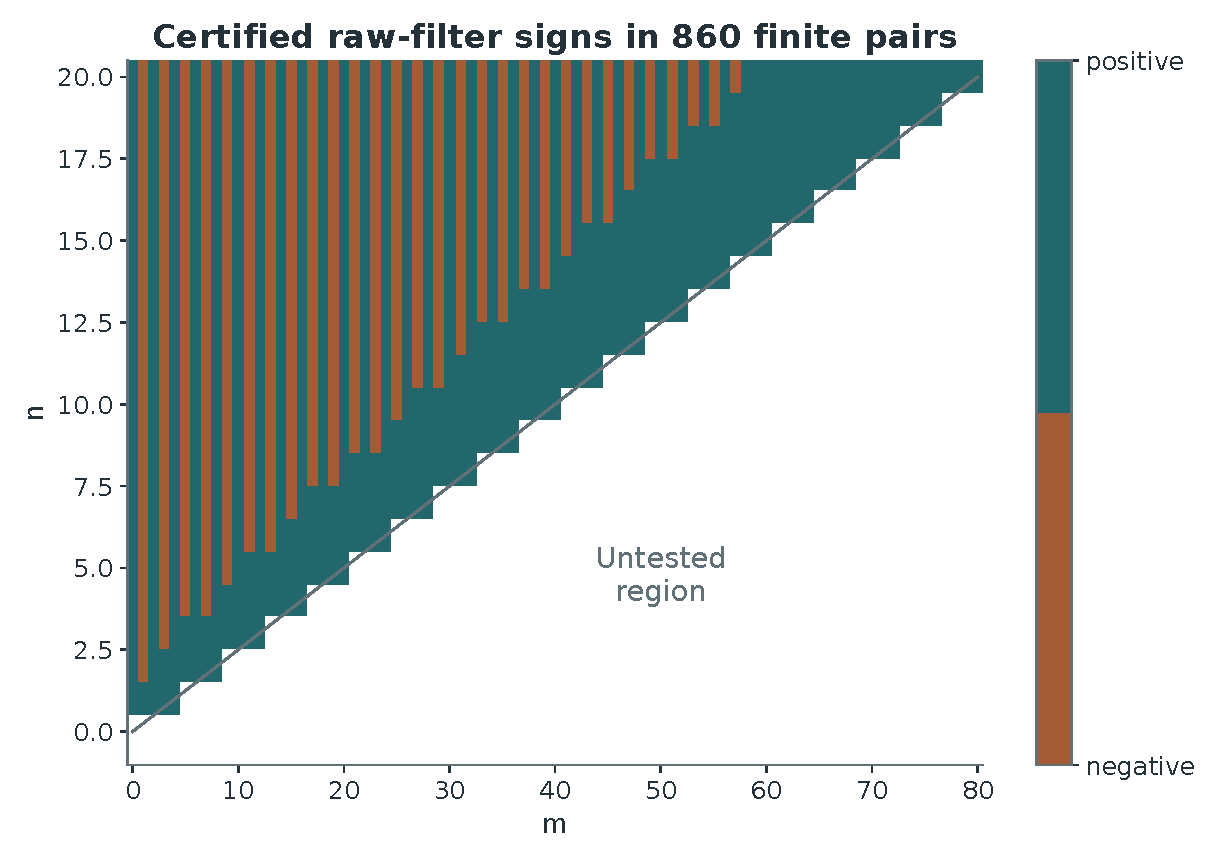
\includegraphics[width=0.91\linewidth]{../visual/figures/27_filter_signs.pdf}
\caption{Certified signs in a bounded packet domain. Even filter orders
have a universal positivity proof. Odd filter orders display both signs,
and the proposed alternating rule fails.}\label{cb_fig_filter_signs}
\end{figure}

\section{The exact historical integer pair}

Let $N=n+m$ and put
\begin{equation}\label{cb_eq_C_clear}
 C_{n,m}=L_{2N}^2.
\end{equation}
The pair produced by the historical script is
\begin{align}
 A_{n,m}&=8(-1)^nC_{n,m}S_{n,m},\label{cb_eq_historical_A}\\
 B_{n,m}&=8(-1)^nC_{n,m}H_{n,m}.
 \label{cb_eq_historical_B}
\end{align}
Both coefficients are integers. Integrality of $A$ follows from that of
$S$. For $B$, each index $k=n+i$ satisfies $k\leq N$, so $L_{2k}$ divides
$L_{2N}$. The sharp source clearing
$4\cdot16^kL_{2k}^2v_k\in\Z$ therefore proves integrality term by term
after multiplication by $8L_{2N}^2$. The binomial weights introduce no
further denominators.

The cleared linear form is exactly
\begin{equation}\label{cb_eq_cleared_integral}
 A_{n,m}G-B_{n,m}
 =C_{n,m}F_{n,m}
 =16^nL_{2N}^2\widetilde J_{n,m}.
\end{equation}
Every factor in this identity has a fixed meaning. In particular, the
historical pair includes the constant factor $8$ and uses the possibly
redundant common clearing $L_{2N}^2$. It is not automatically a primitive
integer pair. Dividing out its common content is a separate arithmetic
operation examined later.

At $m=0$ the construction reduces to the cleared original recurrence form.
At $n=0$ all identities remain valid with $T_0=1$, $v_0=0$, and $L_0=1$.
The large valuation scan starts at $n=1$ for its stated triangular domain,
but that computational choice does not restrict the algebraic identities
proved in this chapter.

\chapter{What the modular valuation scan proves}
\label{cb_ch_modular}

The packet coefficients grow rapidly, but their divisibility by two can be
decided from a sufficiently precise residue. The large scan uses that fact
to evaluate a finite domain efficiently. Its exactness comes from a simple
valuation lemma and from the absence of zero residues. Its limitation comes
from the finite domain. These are separate issues: modular arithmetic can
give an exact answer at millions of pairs without producing a theorem at
every pair.

\section{The residue lemma}

For a nonzero integer $z$, let $v_2(z)$ be the largest nonnegative integer
$t$ such that $2^t$ divides $z$. Thus $v_2(12)=2$ and $v_2(1)=0$.
The value $v_2(0)$ is infinite rather than a finite integer. Our packet
$S_{n,m}$ is strictly positive, so its valuation is always finite, even when
a finite precision residue is zero.

\begin{lemma}[Exactness below the precision ceiling]\label{cb_lem_mod_v2}
Let $K\geq1$, let $z\ne0$ be an integer, and let $\rho$ be its least
nonnegative residue modulo $2^K$. If $\rho\ne0$, then
\[
 v_2(z)=v_2(\rho)<K.
\]
If $\rho=0$, the residue gives only $v_2(z)\geq K$.
\end{lemma}

\begin{proof}
Write $z=\rho+2^Kh$. If $\rho=2^ta$ with $a$ odd and $t<K$, then
$z=2^t(a+2^{K-t}h)$ and the parenthesis is odd. Hence the valuation is
exactly $t$. If $\rho=0$, the congruence says that $2^K$ divides $z$, but
contains no information about further powers of two.
\end{proof}

For example, the residue of $S_{1,1}=2624$ modulo $2^{128}$ is nonzero and
has valuation six. Its residue modulo $16$ is zero, which says only that
its valuation is at least four. The integer itself did not change. The
precision changed the information available about it.

A program that returns a number $K$ for a zero residue must attach a lower
bound interpretation to that number. It must not use it as an exact
valuation or as an exact maximum of the domain. The historical script
counts unresolved residues and includes an explicit exactness flag. The
release tests that flag deliberately.

\begin{figure}[tbp]
\centering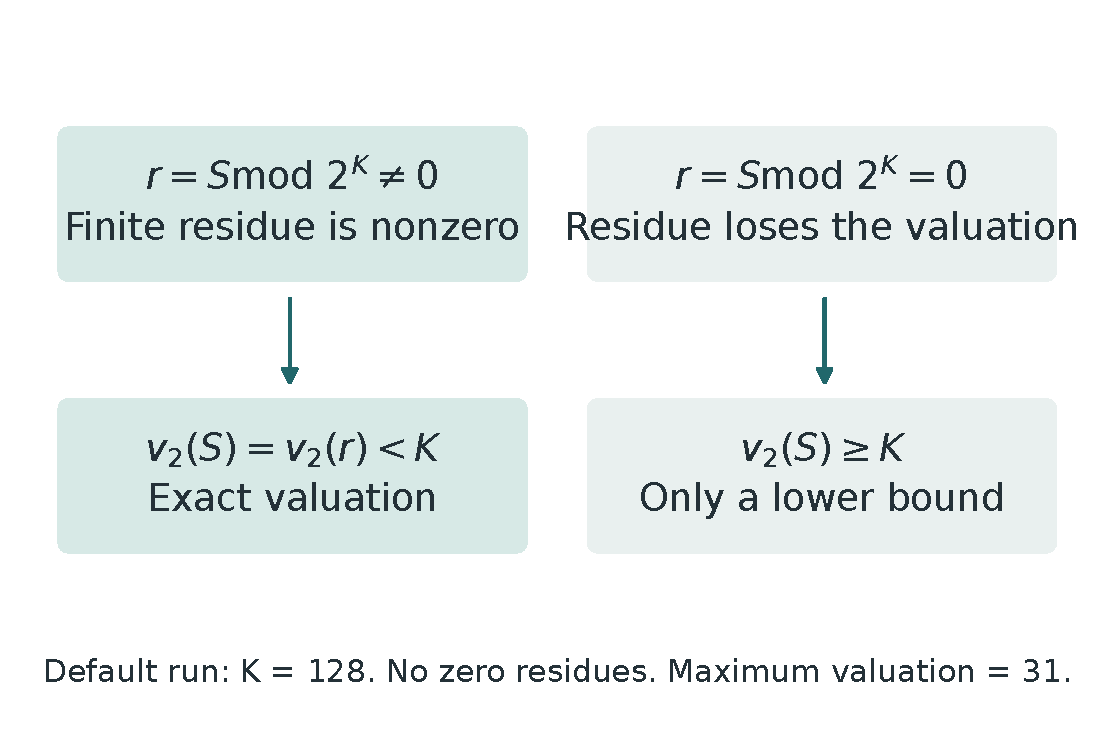
\includegraphics[width=0.91\linewidth]{../visual/figures/18_modular_exactness.pdf}
\caption{A nonzero residue modulo $2^K$ determines the exact valuation.
A zero residue reaches the precision ceiling and supplies only a lower
bound.}\label{cb_fig_mod_exactness}
\end{figure}

\section{The domain and the Pascal computation}

For a positive integer $N$, the scanned domain is
\begin{equation}\label{cb_eq_scan_domain}
 \mathcal D_N=\{(n,m):1\leq n\leq N,\ 0\leq m\leq4n\}.
\end{equation}
The number of scanned pairs is
\begin{equation}\label{cb_eq_scan_count}
 \sum_{n=1}^N(4n+1)=2N^2+3N.
\end{equation}
The upper slope $4$ is part of the experiment's definition. The
scan supplies no information about pairs above this boundary or with
$n>N$.

The computation first constructs $T_0,\ldots,T_{5N}$ through the exact
integer recurrence. It then reduces these integers modulo $2^K$. The
resulting array is the packet row with $m=0$. At each subsequent row,
Pascal evolution replaces adjacent entries by their sum modulo $2^K$.
Induction from \eqref{cb_eq_Pascal} proves that every entry read by the
scan is the exact residue of its packet sum.

For a fixed row $m$, the allowed indices are
\[
 \max(1,\lceil m/4\rceil)\leq n\leq N.
\]
Rows are needed through $m=4N$. In row $m$, the seed array is sufficient
for every $n\leq5N-m$. At the extreme row $m=4N$ this bound is exactly
$n\leq N$. Thus no scanned entry needs an unconstructed seed term.
The algorithm evaluates additional row entries to support later rows.
Those additions do not enlarge the declared set of scanned pairs.

This procedure uses full exact integers to construct the seed sequence,
including checks of all division remainders. Only the subsequent packet
row evolution is performed at fixed modular precision. Describing the
entire calculation as a floating point estimate would therefore be
incorrect. Describing its finite result as a uniform asymptotic theorem
would also be incorrect.

\section{The reproduced 2000 row result}

The historical run takes $N=2000$ and $K=128$. The release reran the
unchanged historical algorithm and compared its result with the recovered
output. The finite arithmetic results agree. In the domain
$\mathcal D_{2000}$ there are exactly $8{,}006{,}000$ pairs. Every observed
residue is nonzero, so the residue lemma applies at every pair. The exact
maximum valuation in this finite domain is
\begin{equation}\label{cb_eq_finite_max}
 \max_{(n,m)\in\mathcal D_{2000}}v_2(S_{n,m})=31.
\end{equation}
The recorded maximizing pair is $(1466,2113)$. The record reports the
first maximum encountered in its scan order and makes no assertion that
this maximizing pair is unique.

There is a generous precision margin: the largest observed valuation is
$31<128$, and there are zero unresolved residues. Consequently the finite
maximum is exact, rather than a maximum of truncated lower bounds. No
statistical confidence interval is involved. The essential qualification
is the finite domain in \eqref{cb_eq_finite_max}.

\begin{figure}[tbp]
\centering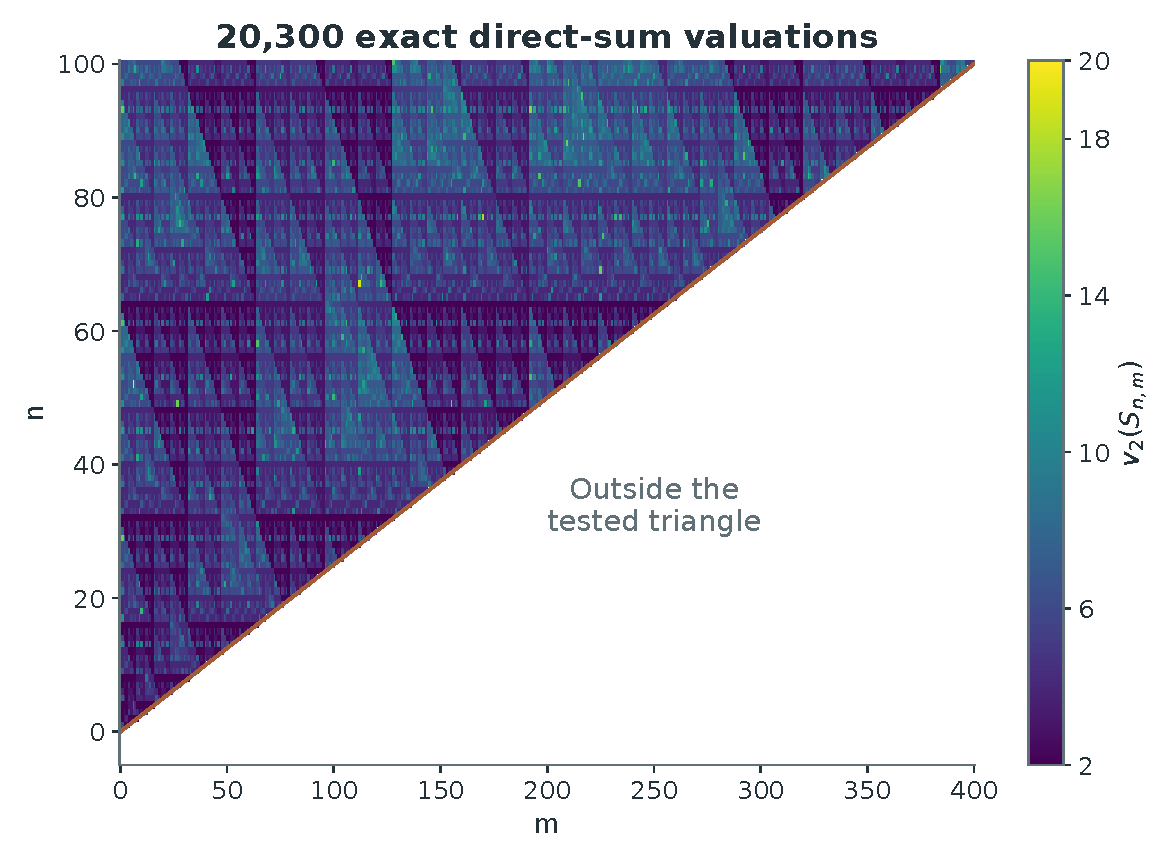
\includegraphics[width=0.93\linewidth]{../visual/figures/19_v2_heatmap.pdf}
\caption{An exact valuation grid in the smaller independently checked
domain. The pattern can suggest questions about cancellation, but its
appearance does not imply an asymptotic law.}\label{cb_fig_v2_grid}
\end{figure}

\section{A comparison at every pair and a full integer witness}

The historical smaller crosscheck reports the same maximum from direct
sums through $N=100$. Matching only two summary maxima would be a weak
comparison: different entry values can share the same maximum. The release
therefore compares every pair in $\mathcal D_{100}$.

For each of its $20{,}300$ pairs, a separate implementation evaluates
\[
 \sum_{i=0}^m\binom miT_{n+i}
\]
as a full positive integer and compares both its residue modulo $2^{128}$
and its exact valuation with the Pascal row entry. All pairs agree. There
are no zero residues. The finite maximum is $20$, recorded first at
$(52,6)$ in the direct comparison's order.

The direct summation and Pascal evolution use different operations on the
same seed data. This catches errors in the packet transform that agreement
between two copies of the same row update could miss. A separately indexed
rational recurrence also checks the seed construction through $n=500$.
These comparisons still share the intended recurrence formulas and require
the literature normalization contract. Their independence is operational,
not a claim that all common source risk has disappeared.

The pair $(1466,2113)$ was additionally evaluated as a full integer, along
with four neighboring pairs. The maximizing witness has bit length
$26{,}743$ and exact valuation $31$. Its complete hexadecimal integer is
included in the evidence bundle with a hash. The neighboring valuations
are much smaller:
\begin{center}
\begin{tabular}{@{}rrr@{}}
\toprule
$n$ & $m$ & $v_2(S_{n,m})$\\
\midrule
$1465$ & $2113$ & $12$\\
$1466$ & $2112$ & $13$\\
$1466$ & $2113$ & $31$\\
$1466$ & $2114$ & $11$\\
$1467$ & $2113$ & $11$\\
\bottomrule
\end{tabular}
\end{center}
These five full integer computations corroborate a particular spike.
They do not establish the maximum over millions of pairs. The exhaustive
modular scan with no unresolved residues establishes that finite maximum.

\section{A deliberate precision failure}

The release includes a diagnostic with $N=3$ and just $K=4$ bits of
precision. There are 27 pairs. Eight residues are zero, so those eight
valuations are unresolved at this precision. The historical scan records
a ceiling value of four and sets its exactness flag to false. Full integer
evaluation shows that the actual finite maximum is six.

This is a successful diagnostic of a deliberately insufficient precision,
not an exact four bit maximum. It demonstrates why the unresolved count
is load bearing. The program's numerical field alone would be misleading
if read without its flag. In the actual 128 bit release run, the same
classification logic reports zero unresolved entries and therefore
permits an exact interpretation.

One should also distinguish this diagnostic from the failed odd filter
sign hypothesis. The low precision test intentionally triggers a known
information limitation and verifies that it is reported correctly. The
odd sign test disproves a proposed mathematical pattern. The evidence
bundle records both, with their different meanings.

\section{Why a finite maximum does not settle growth}

The largest valuation seen so far is small compared with the largest
index. That observation motivates a question such as
\[
 v_2(S_{n,m})=o(n+m)
\]
along a specified family of packet indices. It does not prove the answer.
A universal statement needs quantified control beyond the scanned domain,
with the family of $m$ values and the meaning of uniformity stated
explicitly. A maximum found on a bounded grid cannot rule out later spikes
of a different scale.

Even a proved estimate for $v_2(S_{n,m})$ would address only one prime and
one coefficient. The common content of the full integer pair involves both
coefficients, their clearing factor, and odd prime divisibility. The scan
therefore supplies a precise finite arithmetic fact and a well defined
research question. It is not, by itself, the missing denominator theorem
or an irrationality proof.

The next stage should preserve this clarity. A proposed global valuation
bound must have a written argument valid at every permitted index. A
claimed content improvement must refer to the exact integer pair or to
its primitive reduction. A decay claim must include the clearing factors
that turn a real error into an integer linear form. The finite experiment
can guide those arguments and test their implementations, while the
global conclusion remains subject to its own proof.


\chapter{Primitive content and the cost of clearing}
\label{chap:primitive-content}

\section{Three integers with different jobs}

The packet coefficients are rational before denominators are cleared. Their common divisor depends on the chosen clearing factor. The rational approximation and its primitive integer linear form do not. This distinction is the central arithmetic issue in the five historical gcd calculations.

Fix integers $n,m\geq0$, and write
\begin{equation}
 U=\sum_{i=0}^{m}\binom miT_{n+i},\qquad
 V=\sum_{i=0}^{m}\binom mi16^{n+i}v_{n+i}.
 \label{eq:primitive-UV}
\end{equation}
These are fixed-pair aliases $U=S_{n,m}$ and $V=H_{n,m}$ for the packets defined earlier, not the integral coefficients of a different source normalization. Here $T_k=16^ku_k$ is a positive integer. Consequently $U$ is a positive integer. Write $V=N/D$ in lowest terms, with $D>0$ and $\gcd(N,D)=1$. In the exceptional case $V=0$, the same convention sets $N=0,D=1$. Set
\begin{equation}
 \ell=2(n+m),\qquad L_\ell=\operatorname{lcm}(1,\ldots,\ell),
 \qquad Q=8L_\ell^2,
 \label{eq:Q-clearance}
\end{equation}
with $L_0=1$.

The source arithmetic ensures $QV\in\Z$. Indeed, the strong coefficient theorem gives $4\cdot16^kL_{2k}^2v_k\in\Z$, and $L_{2k}\mid L_\ell$ for $k\leq n+m$. The weaker factor $8$ in $Q$ therefore clears every summand in \eqref{eq:primitive-UV}. Since $V=N/D$ is reduced, this proves $D\mid Q$. The factor $Q$ is a convenient universal choice. The factor $D$ is the actual least denominator of this particular rational packet.

The historical cleared coefficients are
\begin{equation}
 A=(-1)^nQU,\qquad B=(-1)^nQV,
 \qquad g=\gcd(|A|,|B|).
 \label{eq:cleared-pair}
\end{equation}
The sign changes neither the gcd nor the approximation $B/A=V/U$. Finally put
\begin{equation}
 h=\gcd(DU,N).
 \label{eq:minimal-content}
\end{equation}
This is the content of the minimally cleared pair. It must not be confused with $g$. The three quantities $Q$, $D$, and $h$ record, respectively, the chosen clearing factor, the actual packet denominator, and the common content left after minimal clearing.

\section{An exact decomposition}

\begin{proposition}[Redundant clearance and primitive content]
\label{prop:content-decomposition}
For the coefficients above,
\begin{equation}
 h=\gcd(U,N),\qquad
 g=\frac QD\,h.
 \label{eq:gcd-decomposition}
\end{equation}
The reduced rational approximation and primitive coefficients are
\begin{equation}
 \frac VU=\frac{N/h}{DU/h},\qquad
 \frac Ag=(-1)^n\frac{DU}{h},\qquad
 \frac Bg=(-1)^n\frac Nh.
 \label{eq:primitive-pair}
\end{equation}
In particular the positive reduced denominator is $q=DU/h$.
\end{proposition}

\begin{proof}
If $N=0$, the reduced convention gives $D=1$. Since $U>0$, one has $h=U$, $g=QU$, and the unsigned primitive pair is $(1,0)$. All the stated identities follow directly in this case. Assume now $N\ne0$. Since $\gcd(D,N)=1$, multiplication of $U$ by $D$ adds no prime factor that can divide $N$. Prime by prime, $\min\{v_p(DU),v_p(|N|)\}=\min\{v_p(U),v_p(|N|)\}$. This proves the first equality. Next write $Q=cD$, where $c$ is a positive integer. The unsigned cleared pair is $(cDU,cN)$, so its gcd is $c\gcd(DU,N)=ch$. Dividing both coefficients by this gcd proves the remaining identities. The pair $(DU/h,N/h)$ is coprime by the definition of $h$, which proves the claim about the reduced denominator.
\end{proof}

The decomposition contains no asymptotic assumption. It holds at each individual pair $(n,m)$. Its usefulness is that it assigns every common factor to a precise source. A large value of $g$ can be caused by a large value of $Q/D$, even when $h$ is small. Such a factor reflects an unnecessarily generous initial clearing choice. It is not additional content in the minimally cleared pair.

For the historical normalization of the integral filter,
\begin{equation}
 \widetilde J_{n,m}
 =8(-1)^n16^{-n}(UG-V).
 \label{eq:primitive-filter-normalization}
\end{equation}
Thus the primitive integer linear form is
\begin{align}
 \Lambda_{n,m}
 &=\frac AgG-\frac Bg
 =(-1)^n\frac D h(UG-V)\notag\\
 &=\frac{16^nL_\ell^2}{g}\,\widetilde J_{n,m}.
 \label{eq:primitive-error}
\end{align}
Every normalization factor in this formula matters. In particular, the $8$ in $Q$ cancels the $8$ in \eqref{eq:primitive-filter-normalization}. The right side is a real expression for a linear form with integer coefficients. Its absolute value is independent of whether the signs are carried in $A,B$ or in the filter.

\section{Scaling does not manufacture an improvement}

\begin{proposition}[Invariance under additional clearing]
\label{prop:scale-invariance}
If an integer pair $(A,B)$ is replaced by $(cA,cB)$ for an integer $c>0$, then its primitive pair and primitive linear form remain unchanged. More generally, any integer clearing factor $Q'$ divisible by $D$ gives the same unsigned primitive pair $(DU/h,N/h)$.
\end{proposition}

\begin{proof}
The equality $\gcd(cA,cB)=c\gcd(A,B)$ proves the first statement. For the second, apply Proposition~\ref{prop:content-decomposition} with $Q'$ in place of $Q$. The factor $Q'/D$ cancels exactly on division by the new gcd.
\end{proof}

This observation blocks a tempting but invalid arithmetic argument. One can make the cleared gcd arbitrarily large by multiplying both coefficients by a large integer. Doing so also enlarges the error by precisely the same factor. After reduction there is no change. Any proposed gain must be measured in the primitive form \eqref{eq:primitive-error}, or equivalently in the reduced denominator $q=DU/h$.

An elementary example makes the cancellation visible. Take $U=12$ and $V=10/9$. The minimally cleared pair is $(108,10)$ and has gcd $2$. Its primitive pair is $(54,5)$. Clearing instead with $Q=90$ gives $(1080,100)$ and gcd $20$. The apparent tenfold increase in gcd is exactly the tenfold excess in the clearing factor. Both pairs reduce to $(54,5)$ and both represent the approximation $5/54$.

There is still a legitimate role for a redundant clearing factor. It can make a universal theorem easy to state and a program easy to reproduce. The correction is accounting, not a ban on convenient denominators. A calculation with $Q$ is valid when the reduction by $g$ is kept in the same formula. A calculation that counts $g$ as a gain while ignoring the corresponding size of $Q$ is not valid.

\section{The five recovered rows}

The historical script recorded five pairs near the slope used in Eskandari's filter. The fresh exact run reproduces their gcds and factorizations. An independent rational calculation also extracts $D$, $Q/D$, and $h$. The resulting decomposition is as follows.

\begin{table}[htbp]
\centering\small
\begin{tabular}{@{}rrrrr@{}}
\toprule
$(n,m)$ & $Q/D$ & $h$ & $g$ & $v_2(g)$\\
\midrule
$(20,66)$ & $1\,703\,936$ & $8$ & $13\,631\,488$ & $20$\\
$(30,100)$ & $129\,499\,136$ & $4$ & $517\,996\,544$ & $21$\\
$(50,166)$ & $2\,779\,250\,688$ & $8$ & $22\,234\,005\,504$ & $22$\\
$(70,232)$ & $5\,257\,560\,064$ & $64$ & $336\,483\,844\,096$ & $27$\\
$(100,332)$ & $1\,084\,227\,584$ & $8$ & $8\,673\,820\,672$ & $24$\\
\bottomrule
\end{tabular}
\caption{Exact content decomposition at the five historical pairs. These are finite values, not an asymptotic law.}
\label{tab:content-five}
\end{table}

The factorizations of the cleared gcds are
\begin{align*}
13\,631\,488&=2^{20}\cdot13,\\
517\,996\,544&=2^{21}\cdot13\cdot19,\\
22\,234\,005\,504&=2^{22}\cdot3^2\cdot19\cdot31,\\
336\,483\,844\,096&=2^{27}\cdot23\cdot109,\\
8\,673\,820\,672&=2^{24}\cdot11\cdot47.
\end{align*}
For these rows the minimally cleared gcd has only the powers of $2$ displayed in $h$. All odd factors in the listed cleared gcds belong to $Q/D$. That conclusion is specific to these five pairs. It does not establish that odd primitive content is always absent.

The first row illustrates the exact check without printing its very large numerator and denominator. The independently reduced rational packet has denominator
\begin{equation*}
 D=\operatorname{den}\left(\sum_{i=0}^{66}\binom{66}{i}16^{20+i}v_{20+i}\right).
\end{equation*}
Its recorded quotient $Q/D$ is $1\,703\,936$, and the minimal pair has gcd $8$. Multiplication gives $1\,703\,936\cdot8=13\,631\,488$, exactly the historical value. The complete decimal integers $U,N,D,Q$ are retained in the diagnostic JSON. They are inputs to an exact equality check, rather than values inferred from rounded logarithms.

\begin{figure}[htbp]
\centering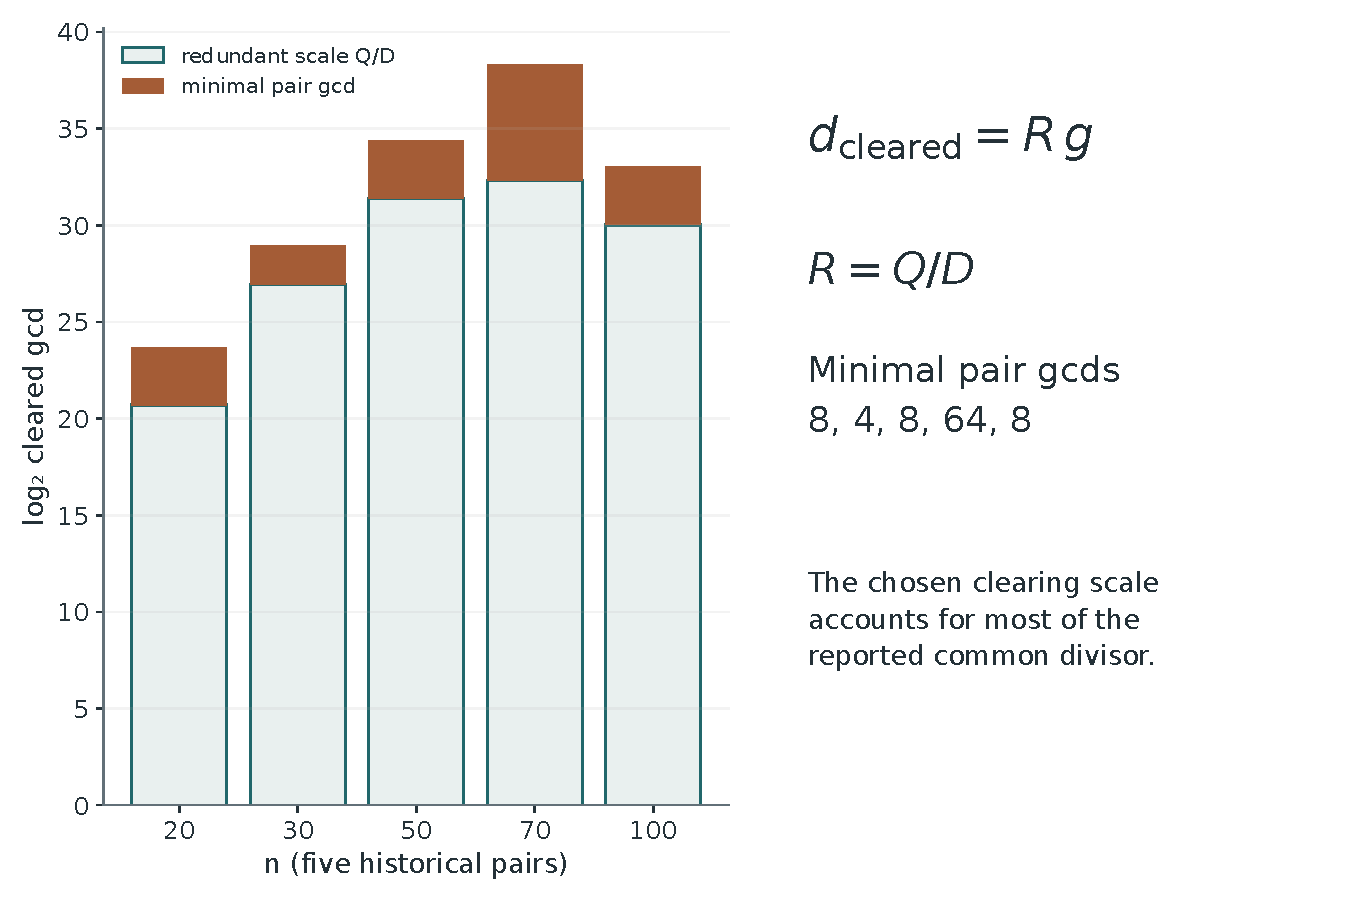
\includegraphics[width=0.96\linewidth]{../visual/figures/24_gcd_decomposition.pdf}
\caption{The cleared gcd splits into redundant scale and content of the minimally cleared pair. Each displayed bar belongs to one of the five exact computations.}
\label{fig:content-decomposition}
\end{figure}

The distinction also affects the dyadic interpretation. At $(20,66)$, $v_2(h)=3$, while $v_2(g)=20$. The remaining seventeen powers of $2$ occur in $Q/D$. At $(70,232)$, the corresponding split is $6+21=27$. A plotted valuation of the cleared gcd does not by itself measure the dyadic content of the packet.

\section{Rates are observations until quantified}

The historical display divides $\log g$ by $n+m$. Its five values decrease from approximately $0.19102$ to $0.05297$. These are useful diagnostics of the sampled pairs. They do not prove $\log g=o(n+m)$, a monotonicity theorem, or a bound at every subsequent pair. Even the sampling rule matters. A result along one sequence $m=m(n)$ is weaker than a bound uniform over a two dimensional range of indices.

\begin{figure}[htbp]
\centering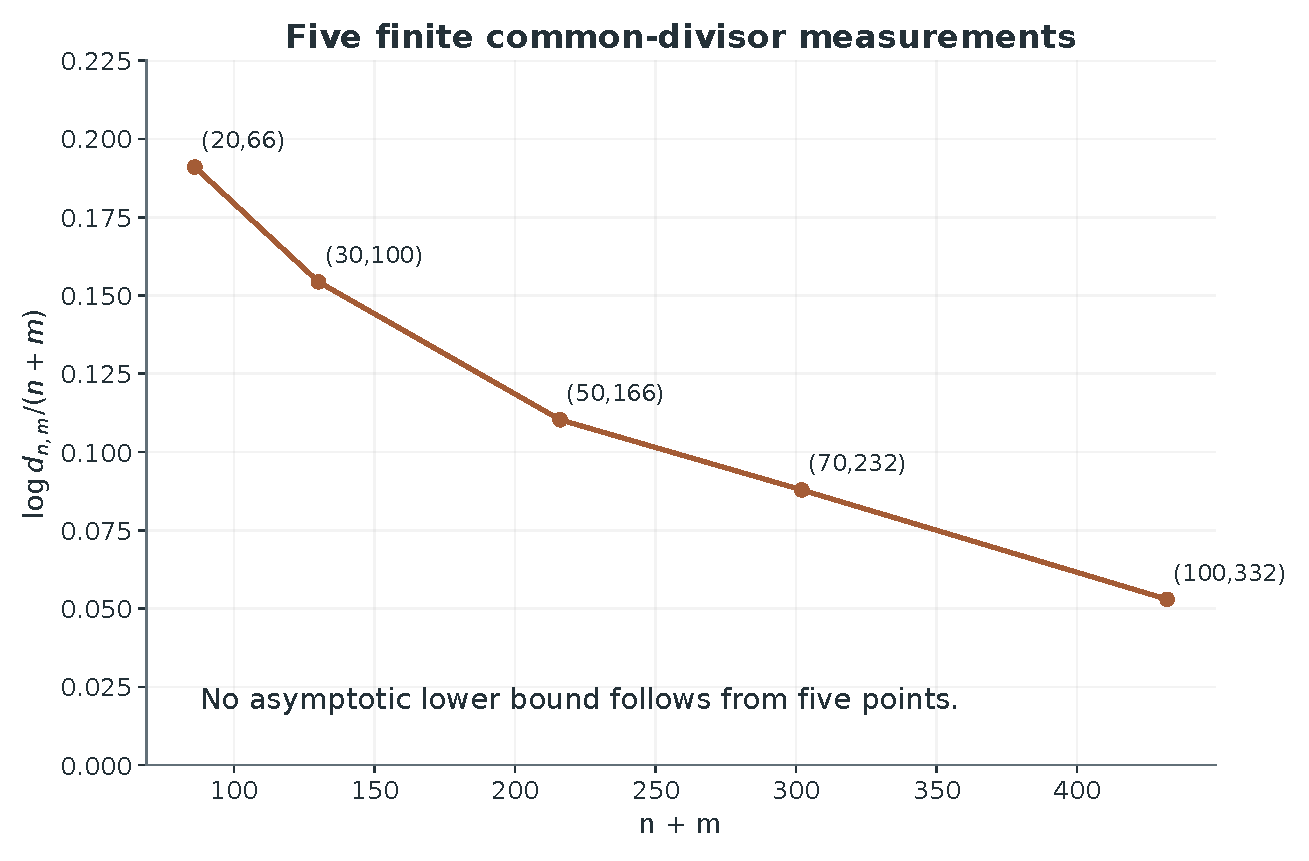
\includegraphics[width=0.96\linewidth]{../visual/figures/23_gcd_rate.pdf}
\caption{The historical logarithmic ratios decrease at the five sampled pairs. The line joins observations and carries no prediction beyond them.}
\label{fig:sampled-content-rate}
\end{figure}

The exact decomposition yields a more informative identity for rate analysis:
\begin{equation}
 \log g=\log Q-\log D+\log h.
 \label{eq:log-content-split}
\end{equation}
Suppose a future proof supplies limits for the three terms on the right along a chosen family. Then \eqref{eq:log-content-split} determines the cleared content rate. At present, the five rows supply values, not those limits. The identity separates the questions that a proof would need to answer. How much smaller is the true packet denominator than the universal denominator? How large is primitive common content? Are the bounds valid along every index in the chosen family?

There is a further one-sided relation to the binomial valuation scan. Because $h\mid U$, one always has $v_2(h)\leq v_2(U)$. If a universal estimate $v_2(U)=o(n+m)$ were proved, it would force the dyadic part of $h$ to be subexponential. It would not control odd factors of $h$, nor the factor $Q/D$. Conversely, a large cleared dyadic gcd can coexist with small $v_2(U)$ because most of its dyadic factor may come from redundant clearance.

This is why neither the large Pascal scan nor the five cleared gcds close the irrationality argument. They examine related arithmetic features, but they do not yet provide a complete uniform estimate for the primitive linear forms. The next chapter states exactly what that estimate must accomplish.

\chapter{The asymptotic bottleneck}
\label{chap:asymptotic-bottleneck}

\section{A nonzero family with an explicit analytic bound}

An irrationality argument needs an infinite family, not simply many successful finite values. For the present filter, a convenient family chooses an even integer $m=m(n)$ with $m/n\to\alpha\geq0$. Evenness supplies nonvanishing by a written integral argument. The slope supplies a definite analytic scale.

Write
\begin{equation}
 \phi=\frac{1+\sqrt5}{2},\qquad t=\phi^{-5},
 \qquad R=16\phi^5=88+40\sqrt5.
 \label{eq:asymptotic-constants}
\end{equation}
The unfiltered integral has the representation
\begin{equation}
 J_k=\int_{[0,1]^2}\psi(x,y)^k\,\dd\mu(x,y),
 \quad
 \psi=\frac{xy(1-x)(1-y)}{1-xy},
 \quad
 \dd\mu=\frac{\dd x\,\dd y}{\sqrt{x(1-y)}(1-xy)}.
 \label{eq:bottleneck-measure}
\end{equation}
The measure has finite total mass $J_0=8G$. The factor $1-xy$ in its denominator lies outside the square root. Moving it inside changes the integral and invalidates the coefficient identification.

Expanding the filter gives
\begin{equation}
 \widetilde J_{n,m}
 =\int_{[0,1]^2}\psi^n(1-16\psi)^m\,\dd\mu.
 \label{eq:bottleneck-filter}
\end{equation}
The range of $\psi$ is contained in $[0,t]$ and reaches its positive maximum $t$. In particular $t>1/16$. The filter factor therefore changes sign within the integration region. When $m$ is even, the integrand is nonnegative. It is strictly positive on an open subset of the interior on which $\psi>0$ and $\psi\ne1/16$. The density of $\mu$ is positive there. Hence
\begin{equation}
 \widetilde J_{n,m}>0\qquad(m\ \text{even}).
 \label{eq:even-filter-positive}
\end{equation}
This is a universal nonvanishing result. It uses neither a decimal value of $G$ nor a finite sign scan. For odd $m$, the same proof does not apply.

\section{Where the two branches of $M$ come from}

For $\alpha\geq0$, define
\begin{equation}
 M(\alpha)=\max\left\{
 \frac{1}{16(1+\alpha)}
 \left(\frac\alpha{1+\alpha}\right)^\alpha,
 \ t(16t-1)^\alpha
 \right\}.
 \label{eq:M-alpha}
\end{equation}
At $\alpha=0$ the first expression is assigned its continuous value $1/16$. This avoids treating the displayed $0^0$ as an algebraic input. The formula is Eskandari's source bound, with the recurrence normalization translated explicitly in LC06 and LC07~\cite{Eskandari2026}.

It can also be understood directly from the filter. On $0\leq s\leq1/16$, maximize $s(1-16s)^\alpha$. For $\alpha>0$, logarithmic differentiation gives
\begin{equation*}
 \frac1s-\frac{16\alpha}{1-16s}=0,
 \qquad s=\frac{1}{16(1+\alpha)}.
\end{equation*}
Substituting this point gives the first branch in \eqref{eq:M-alpha}. The endpoints give zero for $\alpha>0$, so this critical point is the maximum. At $\alpha=0$, the maximum on the interval is its right endpoint $1/16$.

On $1/16\leq s\leq t$, maximize $s(16s-1)^\alpha$. For $\alpha>0$ its logarithmic derivative is
\begin{equation*}
 \frac1s+\frac{16\alpha}{16s-1}>0.
\end{equation*}
Its maximum is therefore $t(16t-1)^\alpha$. The same conclusion holds at $\alpha=0$ because the function is then $s$. These two regions explain both branches and the need to retain their maximum.

Let $\alpha_n=m(n)/n$. The finite measure in \eqref{eq:bottleneck-filter} gives
\begin{equation}
 |\widetilde J_{n,m(n)}|
 \leq 8G\,M(\alpha_n)^n.
 \label{eq:actual-M-bound}
\end{equation}
Continuity of the two branches, including their stated extension at zero, then proves
\begin{equation}
 \limsup_{n\to\infty}
 |\widetilde J_{n,m(n)}|^{1/n}\leq M(\alpha).
 \label{eq:M-limsup}
\end{equation}
This is an upper bound. An equality for the actual integral would require a further argument. In particular, an upper bound does not measure the effect of sign cancellation in an odd filter.

\section{The external denominator scale}

The prime number theorem supplies the standard asymptotic~\cite{Zagier1997}
\begin{equation}
 \log L_k=k+o(k).
 \label{eq:PNT-LCM}
\end{equation}
Indeed $\log L_k=\sum_{p^a\leq k}\log p$ is the Chebyshev function $\psi_{\rm Ch}(k)$, and its ratio to $k$ tends to one. Source contract LC10 records the prime number theorem and the elementary prime power conversion. Equivalently, write $\log L_k=\sum_{a\geq1}\vartheta(k^{1/a})$, where $\vartheta(x)=\sum_{p\leq x}\log p$. The first term is $k+o(k)$. The remaining terms are $O(\sqrt{k}\log k)=o(k)$, using $\vartheta(x)=O(x)$ and at most $\log_2 k$ nonzero terms. The symbol $\psi_{\rm Ch}$ here denotes the arithmetic function, not the two variable kernel in \eqref{eq:bottleneck-measure}. The prime number theorem is an external theorem. The finite lcm calculations in this publication do not reprove it.

Set
\begin{equation}
 K_n=16^nL_{2(n+m(n))}^2.
 \label{eq:K-asymptotic}
\end{equation}
For $m(n)/n\to\alpha$, \eqref{eq:PNT-LCM} gives
\begin{equation}
 \frac{\log K_n}{n}\longrightarrow
 \kappa_0(\alpha)=\log16+4(1+\alpha).
 \label{eq:kappa-alpha}
\end{equation}
The factor $4$ has a precise origin. The lcm index is $2(n+m)$, and the lcm is squared. Missing either factor would create an incorrect apparent decay margin. The subscript in $\kappa_0$ emphasizes that this is the clearing cost alone. Define the combined bound exponent by $E(\alpha)=\kappa_0(\alpha)+\log M(\alpha)$.

With the cleared gcd $g_n=g_{n,m(n)}$, the primitive form is exactly
\begin{equation}
 \Lambda_n=\frac{K_n}{g_n}\widetilde J_{n,m(n)}.
 \label{eq:Lambda-bottleneck}
\end{equation}
Suppose a future arithmetic argument establishes
\begin{equation}
 \delta=\liminf_{n\to\infty}\frac{\log g_n}{n}.
 \label{eq:delta-content}
\end{equation}
For finite $\delta$, the present analytic estimate yields
\begin{equation}
 \limsup_{n\to\infty}\frac{\log|\Lambda_n|}{n}
 \leq\kappa_0(\alpha)+\log M(\alpha)-\delta.
 \label{eq:margin-inequality}
\end{equation}
The same interpretation applies when $\delta=+\infty$: any sufficiently large finite lower bound for the content rate would suffice. All logarithms of nonzero forms are legitimate for the even family by \eqref{eq:even-filter-positive}. The strict negativity of the right side is the missing sufficient margin. A zero margin would not suffice, because lower order terms could still prevent convergence to zero.

\section{What the current bound fails to supply}

Even without numerical optimization, the explicit bound reveals a limitation. Its cleared exponent before content reduction is positive for every slope.

\begin{proposition}[The displayed upper bound has no cleared decay margin]
\label{prop:positive-cleared-upper}
For every $\alpha\geq0$,
\begin{equation}
 \kappa_0(\alpha)+\log M(\alpha)>0.
 \label{eq:positive-bound-rate}
\end{equation}
This statement concerns the exponent of the available upper bound. It is not a lower bound on the actual primitive forms.
\end{proposition}

\begin{proof}
Put $c=16t-1$. The second branch in \eqref{eq:M-alpha} gives
\begin{equation*}
 \kappa_0(\alpha)+\log M(\alpha)
 \geq 4+\log(16t)+\alpha(4+\log c).
\end{equation*}
Now $t=(5\sqrt5-11)/2>5/64$. For example, this inequality follows by squaring the positive rational bound $\sqrt5>357/160$, since $5\cdot160^2>357^2$. Thus $16t>5/4>1$ and $c>1/4$. Consequently the last display is greater than $4+\alpha(4-\log4)>0$.
\end{proof}

The proposition says that the direct combination of $M$ with the chosen denominator bound does not prove shrinking integer forms without a quantified content gain. It does not say that the actual forms diverge. A growing upper bound is compatible with a quantity that decays rapidly. Stronger analytic estimates or smaller actual denominators can change the conclusion, but each requires its own proof.

At the source's approximately optimal slope $\alpha=3.31765$, the two branches of $M$ are near $0.006040$. The resulting exponent $\kappa_0+\log M$ is about $14.93384$ per unit $n$. These are rounded evaluations of explicit formulas, not certified extrema or an estimate for $\log|\Lambda_n|/n$. They show how large a content rate would need to be for this particular upper bound to force decay. The five observed gcd ratios are reported per $n+m$ and cannot be substituted as asymptotic rates in this calculation.

\begin{figure}[htbp]
\centering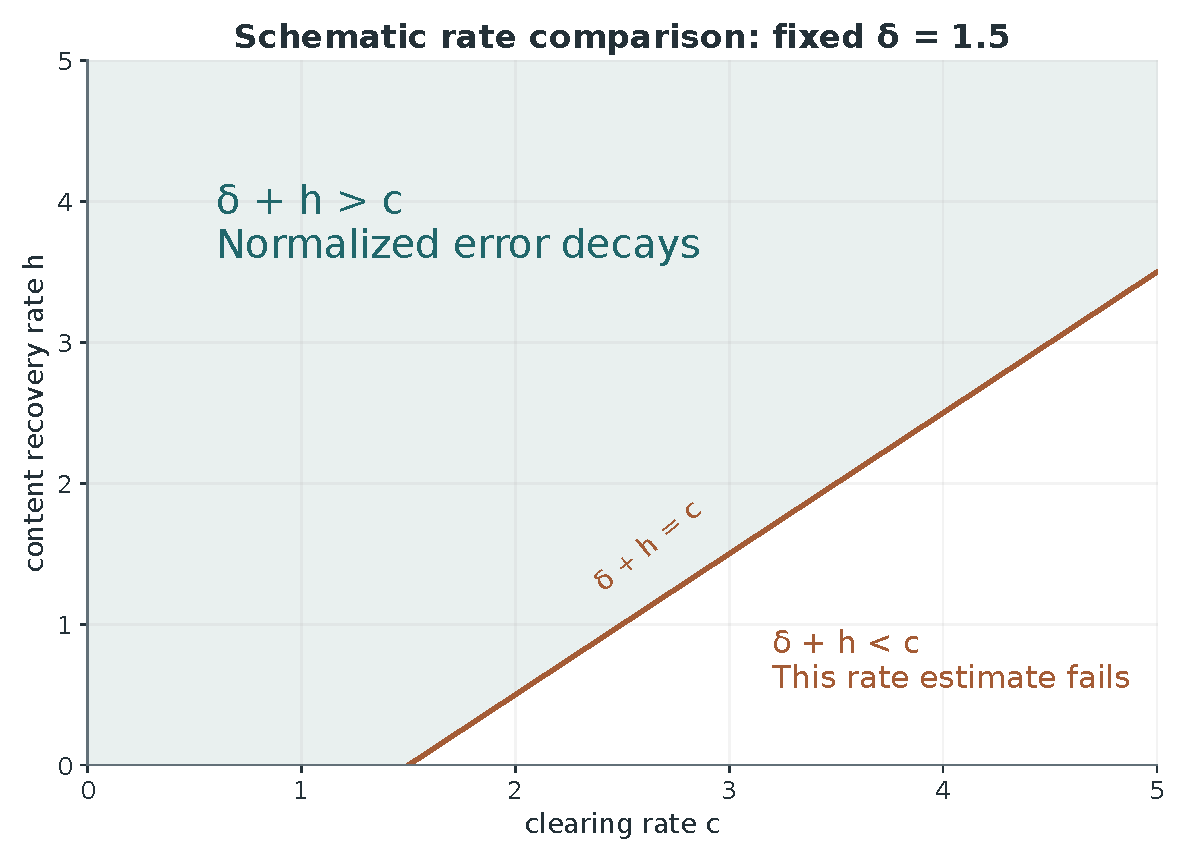
\includegraphics[width=0.96\linewidth]{../visual/figures/25_threshold_plane.pdf}
\caption{A strict negative margin is sufficient for decay after clearing and reduction. The boundary compares exponential rates. Finite measurements do not establish a point's asymptotic location.}
\label{fig:threshold-margin}
\end{figure}

\section{The source approximation exponent}

Eskandari's coefficient growth statement is
\begin{equation}
 \lim_{n\to\infty}\frac{\log|\widetilde U_{n,m(n)}|}{n}
 =\gamma(\alpha)
 =-\log16+\log R+\alpha\log(1+R),
 \label{eq:gamma-alpha}
\end{equation}
where $\widetilde U=8(-1)^n16^{-n}U$. This is an external asymptotic result in the preprint, not a conclusion of the finite recurrence audit. Together with the filter bound it controls the approximation error
\begin{equation}
 \left|G-\frac VU\right|
 =\frac{|\widetilde J|}{|\widetilde U|}.
 \label{eq:approximation-error}
\end{equation}
Before any additional quantified gcd saving, the reduced denominator $q$ is at most the absolute cleared coefficient $|A|$. Its available exponent is
\begin{equation}
 c_A(\alpha)=4(1+\alpha)+\log R+\alpha\log(1+R).
 \label{eq:cA-alpha}
\end{equation}
The source's resulting guaranteed approximation exponent is
\begin{equation}
 \eta(\alpha)=
 \frac{\log R+\alpha\log(1+R)-\log16-\log M(\alpha)}
 {4(1+\alpha)+\log R+\alpha\log(1+R)}.
 \label{eq:eta-alpha}
\end{equation}
The source reports a maximum near $0.62335$ at $\alpha\approx3.31765$ and states its theorem in the rounded form $\eta\geq0.62$~\cite{Eskandari2026}. The present edition records that as a preprint result with its stated dependencies. It does not upgrade it to a peer reviewed theorem, a certified global numerical maximum, or an irrationality proof.

The denominator index in \eqref{eq:eta-alpha} is $n$, while the filter depth grows like $\alpha n$. This is why the lcm term is $4(1+\alpha)$ rather than $4$. Replacing $n$ by $n+m$ consistently rescales every rate. Rescaling just one term changes the statement and is invalid.

An approximation exponent below one cannot contradict rationality. If $G=a/b$ were rational and $p/q\ne a/b$ were reduced, then
\begin{equation}
 \left|\frac ab-\frac pq\right|
 =\frac{|aq-bp|}{bq}\geq\frac1{bq}.
 \label{eq:rational-approx-lower}
\end{equation}
A bound of order $q^{-0.62}$ is larger than this obstruction for large $q$. Even rational numbers have many distinct approximations of that quality. For example $a/b+1/(bk)$ has error $1/(bk)$ and, after reduction, denominator at most $bk$. Nothing in such a bound isolates irrationality.

The identity $c_A-\gamma=\kappa_0$ gives another way to read the threshold. The unreduced exponent satisfies $\eta>1$ exactly when $\kappa_0+\log M<0$. Proposition~\ref{prop:positive-cleared-upper} shows why the displayed source estimate does not reach that regime. A genuine content saving changes the denominator and the primitive error together. It cannot be inserted in just one side of the comparison.

\section{A precise conditional completion theorem}

\begin{theorem}[Sufficient content margin]
\label{thm:conditional-completion}
Choose even integers $m(n)\geq0$ such that $m(n)/n\to\alpha\geq0$. Use the coefficient clearing theorem, the corrected filter identity, and the prime number theorem as specified above. If there exists a real number $\delta_0$ with
\begin{equation}
 \liminf_{n\to\infty}\frac{\log g_{n,m(n)}}{n}\geq\delta_0
 \quad\text{and}\quad
 \delta_0>\kappa_0(\alpha)+\log M(\alpha),
 \label{eq:conditional-content-hypothesis}
\end{equation}
then $G$ is irrational.
\end{theorem}

\begin{proof}
The coefficient clearing theorem and division by the exact gcd make $\Lambda_n=a_nG-b_n$ with $a_n,b_n\in\Z$. Evenness of $m(n)$ makes $\widetilde J_{n,m(n)}>0$, so \eqref{eq:Lambda-bottleneck} gives $\Lambda_n>0$. Choose $\varepsilon>0$ so that $3\varepsilon<\delta_0-\kappa_0(\alpha)-\log M(\alpha)$. For all sufficiently large $n$, the clearing asymptotic gives $K_n\leq\exp((\kappa_0+\varepsilon)n)$, the filter bound gives $|\widetilde J_{n,m(n)}|\leq\exp((\log M+\varepsilon)n)$, and the liminf assumption gives $g_{n,m(n)}\geq\exp((\delta_0-\varepsilon)n)$. Therefore
\begin{equation*}
 0<\Lambda_n\leq
 \exp\bigl((\kappa_0+\log M-\delta_0+3\varepsilon)n\bigr)
 \longrightarrow0.
\end{equation*}
If $G=a/b$ with integers $a,b$ and $b>0$, then $b\Lambda_n=aa_n-bb_n$ is a positive integer. It is at least one, so $\Lambda_n\geq1/b$. This contradicts the displayed convergence.
\end{proof}

The proof of this implication is complete. Its content hypothesis is not established here. The theorem is therefore conditional, and cannot be listed as a proof of the conjecture. It supplies a concrete target for a future arithmetic result. A stronger analytic bound could replace $M$, provided it were proved for the same infinite family and retained the nonvanishing input.

There is also a formulation independent of the universal clearing choice. With $D_n,h_n$ as in Chapter~\ref{chap:primitive-content}, the primitive error is $(-1)^n(D_n/h_n)(S_{n,m(n)}G-H_{n,m(n)})$. An estimate directly on that expression would suffice. If denominator reduction yields a provably smaller exponential cost, the excess factor $Q_n/D_n$ should simply be removed from the accounting. The irrationality criterion itself is unchanged.

\begin{figure}[htbp]
\centering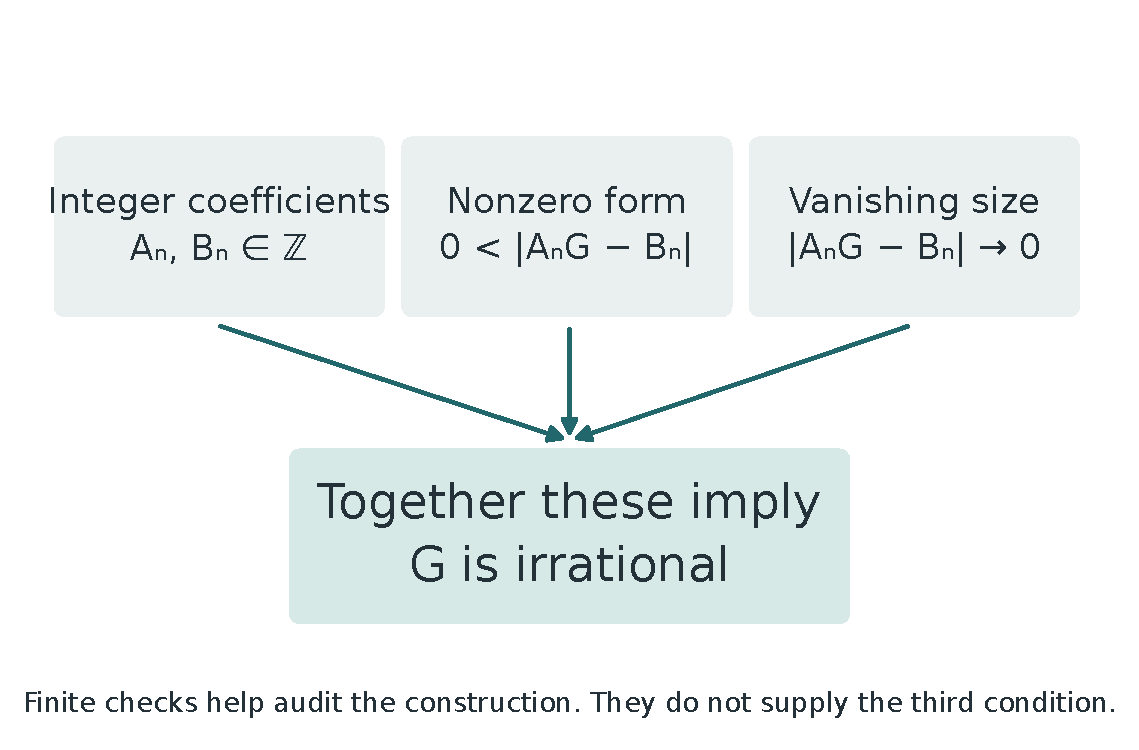
\includegraphics[width=0.96\linewidth]{../visual/figures/28_conditional_route.pdf}
\caption{The conditional route separates integer coefficients, nonvanishing, and a strict decay margin. The first two have stated source or written proofs here. The final global estimate remains open.}
\label{fig:conditional-route}
\end{figure}

\section{Why a finite prefix cannot supply the final hypothesis}

There is a simple logical reason to resist extrapolation. Given any finite list of positive values $x_1,\ldots,x_N$, it has a positive extension that tends to zero and another positive extension that tends to infinity. Keep the list fixed and set the tail to $e^{-n}$ in the first case or $e^n$ in the second. Similarly, any finite list of positive integer gcds can be extended by $1$ forever or by integers with an arbitrarily prescribed positive exponential rate.

These extensions are not asserted to satisfy the Catalan recurrence. They illustrate a narrower point: finite values by themselves do not imply an asymptotic property. The recurrence, integral, or arithmetic structure must supply the bridge. A theorem using that structure could settle a uniform estimate. The prefix alone cannot.

A positive exponent in an upper bound has the same logical limitation. If $x_n\leq e^{cn}$ with $c>0$, both $x_n=e^{-n}$ and $x_n=e^{cn/2}$ satisfy the bound eventually. One sequence decays and the other grows. Thus the failure of the bound to force decay is a proved limitation of the estimate, not proof of divergence of the object it bounds.

\begin{figure}[htbp]
\centering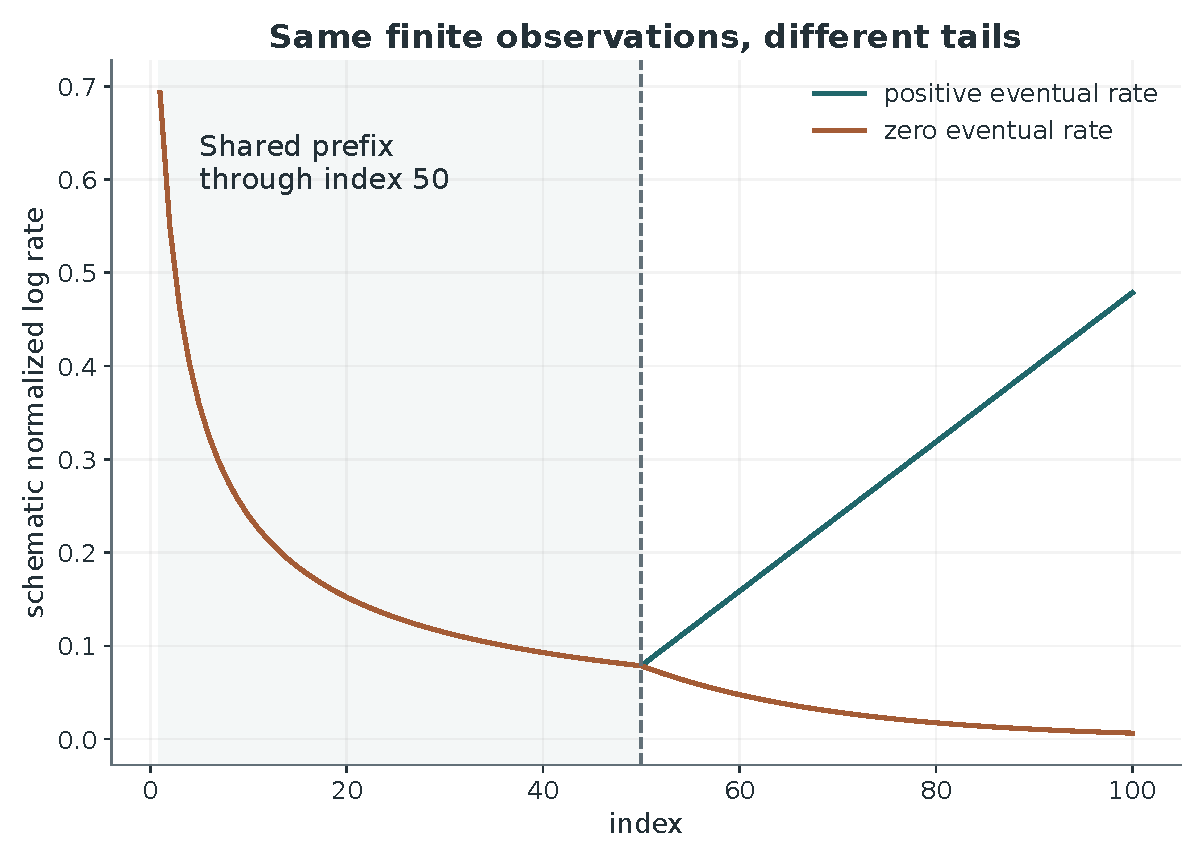
\includegraphics[width=0.96\linewidth]{../visual/figures/26_finite_countermodels.pdf}
\caption{Finite data can agree with incompatible asymptotic extensions. The illustrated tails are logical examples, not alternative Catalan recurrences.}
\label{fig:finite-countermodels}
\end{figure}

The same caution applies to the modular scan. Its $8\,006\,000$ exact valuations establish a large finite statement. They do not prove $v_2(S_{n,m})=o(n+m)$ outside the scanned domain, a uniform bound on odd common factors, or the lower bound on $\log g$ in Theorem~\ref{thm:conditional-completion}. The achievement is reproducible bounded evidence and a sharply stated remaining implication.

\chapter{Evidence, status, and the next theorem}
\label{chap:evidence-status}

\section{What this edition establishes}

This publication assembles three different kinds of mathematical evidence. Written arguments establish identities and implications for all indices under their stated hypotheses. Source contracts identify external theorems and the precise normalization used to apply them. Exact computations establish statements on bounded ranges. These kinds of evidence reinforce one another, but they have different scopes.

The universal arguments written in this edition include the elementary half-binomial denominator lemma, the Wronskian induction, the Pascal identity, the modular valuation criterion, the primitive content decomposition, and the conditional irrationality implication. Some of these arguments start from externally supplied identities. For example, the integrality proof for $T_n$ uses the authenticated half-binomial expression for $u_n$. Its universal arithmetic step is written here, while the identity identifying that expression with the recurrence is an external input.

The integral normalization receives special attention because the printed source contains a factor discrepancy. In the historical recurrence normalization, the correct relation is
\begin{equation}
 u_nG-v_n=\frac{(-1)^n}{8}J_n.
 \label{eq:status-normalization}
\end{equation}
The printed factor $1/4$ is incompatible with $u_0=1$ and the exact evaluation $J_0=8G$. The source audit also checks the all-index normalization through the displayed hypergeometric transformation and partial-fraction coefficient identification. This is an explicit correction with stated dependencies. It is not a silently altered quotation, nor a claim that a published erratum was recovered.

The same separation applies to asymptotic results. The recurrence's growth rates, its limit identification, strong coefficient clearing, and the prime number theorem are external inputs. The exact translation of those results and their combination into an irrationality criterion are written project arguments. No amount of finite recurrence agreement alone proves the externally supplied limit or denominator theorem.

\begin{table}[htbp]
\centering\small
\begin{tabularx}{\linewidth}{@{}p{0.29\linewidth}X@{}}
\toprule
Evidence class & Meaning in this edition\\
\midrule
Written universal argument & A proof applies to every index in its stated domain. External premises remain named.\\
External source input & An authenticated result is translated with its exact initial conditions, factors, and index range.\\
Finite exact computation & Integer or rational decisions are verified only at the recorded inputs.\\
Rounded diagnostic display & Decimal logarithms and plots illustrate exact data or formulas. Their last digits are not theorem inputs.\\
Open estimate & A uniform asymptotic statement is specified, but not established.\\
\bottomrule
\end{tabularx}
\caption{Evidence classes used throughout the publication. The classification concerns the claim, not the prestige of its format.}
\label{tab:evidence-classes}
\end{table}

\section{The finite record}

The historical default run is reproduced without editing the historical program. Its new result JSON is byte for byte identical to the recovered result JSON. This is a strong implementation check for the recorded defaults, not a universal arithmetic theorem.

The large modular scan covers $1\leq n\leq2000$ and $0\leq m\leq4n$, a total of $8\,006\,000$ pairs. It finds maximum valuation $31$, with a witness at $(1466,2113)$ in the historical traversal order. No residue is zero modulo $2^{128}$, so every scanned valuation is below the precision ceiling and is exact. The direct witness calculation reconstructs the full integer sum and verifies the same valuation. The evidence does not assert that this maximizing pair is unique.

The smaller direct grid contains $20\,300$ pairs with $n\leq100$. It agrees with the modular Pascal computation at every pair and has maximum valuation $20$ at $(52,6)$ in its own traversal order. A deliberate low precision test at modulus $2^4$ produces eight zero residues in the much smaller domain $n\leq3$. These are correctly marked unresolved. The true direct maximum there is $6$, while the clipped residue report is $4$. This negative control checks that the program does not mistake a precision ceiling for an exact valuation.

Independent rational recurrence calculations agree through $n=500$. The integer recurrence for $T_n$ has zero remainder at every division through $n=10000$. The half-binomial check verifies all $1\,326$ summands through $n=50$. These finite checks support the implementation and normalization. Their universal counterparts still depend on the written arguments and external coefficient identity.

The five gcd computations in Chapter~\ref{chap:primitive-content} are exact rational calculations, including complete numerator and denominator strings. The displays of $\log g/(n+m)$ are ordinary rounded logarithms. The exact factorization and decomposition are the arithmetic evidence. The display ratios are explanatory summaries.

\section{The failed sign guess remains part of the record}

A diagnostic guess proposed during this audit asserted $\operatorname{sign}F_{n,m}=(-1)^m$ for the raw packet form
\begin{equation}
 F_{n,m}=8(-1)^n\bigl(S_{n,m}G-H_{n,m}\bigr).
 \label{eq:status-raw-F}
\end{equation}
It fails. Already at $(n,m)=(1,1)$,
\begin{equation}
 F_{1,1}=\frac{173056}{9}-20992G>0,
 \label{eq:status-sign-counterexample}
\end{equation}
while the guess predicts a negative sign. A certified rational interval for $G$ determines the sign. Among the $860$ tested pairs with $1\leq n\leq20$ and $0\leq m\leq4n$, there are $138$ mismatches with the guess. All $860$ actual forms are nevertheless certified nonzero.

The failed guess was an exploratory diagnostic of this audit. It was not an authenticated source theorem. Its failure does not contradict the even-filter positivity proof, which has a different hypothesis and a direct integral justification. It does show why a proposed odd-filter sign rule cannot be carried into a global proof on the strength of a suggestive pattern.

The initial independent run retained every mismatch but gave the sign experiment an overly broad interpretive label. The corrected source and final rerun explicitly record falsification. Both runs are preserved. The publication uses the final interpretation and does not conceal the earlier label. The evidence report identifies the final independent directory as the current record.

\section{A dated statement about recent claims}

The edition date matters because recent primary preprints discuss the irrationality of $G$. Zhi-Wei Sun's preprint, submitted on 3 September 2026, claims a proof~\cite{Sun2026}. The checked arXiv history contained only version 1 on 9 October 2026. A subsequent note by Dane Wachs, submitted on 16 September and dated 15 September internally, identifies a gap in a displayed asymptotic derivation~\cite{Wachs2026}. It describes a quadratic contribution from the prime $2$ that it says the derivation does not account for.

These are attributed statements about the checked sources. This publication does not independently reproduce the determinant computations in the critical note. It does not treat that note as a universal theorem excluding every repair, nor import the claimed irrationality theorem from the first preprint. Neither source is described here as peer reviewed.

As of 9 October 2026, no proof of the irrationality of Catalan's constant is established by the material checked for this publication. A primary preprint claims a proof, and a subsequent primary note identifies an incomplete derivation. This edition does not resolve that dispute. A later verified result would require updating this dated status statement.

The source search is bounded. It checked the listed arXiv identifiers, relevant journal and author pages, the recurrence and denominator papers, and the filter preprint. It is not an exhaustive historical survey or a global novelty certification. Where a result is standard or already appears in a source, the edition says so. The filter is attributed to Eskandari. The recurrence and its asymptotic identification are attributed to Zudilin. The strong arithmetic theorem is attributed to Krattenthaler and Rivoal.

\section{What was recovered and what was reconstructed}

The historical project material recovered for this piece consists of the packet audit script, its result JSON, and its run log. Those files are preserved byte for byte. They establish a genuine earlier computational record. They do not contain a recovered monograph, a complete universal proof of irrationality, or a compiled Lean development.

The exposition in this edition is newly reconstructed around that record. It supplies mathematical context, explicit normalization checks, written arithmetic arguments, independent finite checks, source contracts, and a precise remaining asymptotic implication. This reconstruction is part of the publication work. It must not be backdated or presented as prose recovered from the original research session.

The companion source bundle contains the publication source, figure programs, public computation programs, exact outputs, and audit records. Primary papers are cited and their relevant contracts are documented. Complete downloaded third-party papers are not included in the public bundle. There is no Lean compiler certificate for this Catalan piece, because no such formalization was recovered or built for it. A written proof and a successful Python run are reported in their own categories.

\section{The next theorem has a precise shape}

The remaining target is not the vague instruction to find more cancellation. One possible completion is Theorem~\ref{thm:conditional-completion}: choose a specified even family, establish a uniform content rate, and prove a strict negative primitive error margin. Another possibility is a stronger analytic estimate that yields the same integer-form decay after the actual denominator cost is included. A third is a smaller denominator theorem for the filtered coefficients. Each route must retain the exact coefficient normalization and nonvanishing input.

The work can therefore be advanced in distinct, testable directions. An arithmetic route should distinguish $Q/D$ from $h$ and control both dyadic and odd factors where necessary. An analytic route should prove a bound for the actual integral along an infinite family, rather than infer decay from a plot. A formal route should encode the exact statements and mark external asymptotic inputs explicitly. More computation can expose candidates or counterexamples, but it must continue to state its range.

This edition is ready as an audited research account. Its identities, finite record, external dependencies, and open estimates are separated closely enough that a later result can be inserted at a definite point. The irrationality conclusion is not one of its established claims.



\appendix
\chapter{Formula and source reference}
\label{app:formula-reference}

\section{Recurrence and initial values}

The normalized rational sequences start with
\begin{equation}
 (u_0,u_1)=(1,7/4),\qquad(v_0,v_1)=(0,13/8).
 \label{eq:app-initial}
\end{equation}
For $n\geq1$, set
\begin{align}
 p(n)&=20n^2-8n+1,\notag\\
 q(n)&=3520n^6+5632n^5+2064n^4\notag\\
 &\hspace{1.6em}-384n^3-156n^2+16n+7,\notag\\
 a_n&=(2n+1)^2(2n+2)^2p(n),\notag\\
 c_n&=(2n-1)^2(2n)^2p(n+1).
 \label{eq:app-recurrence-coeffs}
\end{align}
Each sequence $w=u$ or $w=v$ obeys
\begin{equation}
 a_nw_{n+1}=q(n)w_n+c_nw_{n-1}.
 \label{eq:app-recurrence}
\end{equation}
The forward recurrence is used only at $n\geq1$. Its coefficients $a_n$ are positive there. The first additional terms are
\begin{equation}
 u_2=\frac{649}{64},\quad u_3=\frac{19471}{256},\qquad
 v_2=\frac{10699}{1152},\quad v_3=\frac{8025653}{115200}.
 \label{eq:app-small-sequences}
\end{equation}

The Wronskian in this edition uses the orientation
\begin{equation}
 W_n=u_{n+1}v_n-u_nv_{n+1}
 =\frac{(-1)^{n+1}p(n+1)}{2(2n+1)^2(2n+2)^2}.
 \label{eq:app-Wronskian}
\end{equation}
Reversing its two terms reverses the sign. The formula applies to $n\geq0$, with the base case supplied by the initial pair and the induction step supplied by \eqref{eq:app-recurrence}.

\section{Integer packets and integrals}

Set $T_n=16^nu_n$. Its forward recurrence is
\begin{equation}
 a_nT_{n+1}=16q(n)T_n+256c_nT_{n-1},
 \qquad T_0=1,\quad T_1=28.
 \label{eq:app-T-recurrence}
\end{equation}
The initial terms are $1,28,2596,311536$. The universally integral expression is
\begin{equation}
 u_n=\sum_{j=0}^n\binom nj
 \binom{n-\tfrac12}{j}\binom{n+j-\tfrac12}{j},
 \label{eq:app-half-binomial}
\end{equation}
with the external coefficient identity and the written half-binomial denominator argument kept distinct.

For $n,m\geq0$, the integer and rational packets are
\begin{equation}
 S_{n,m}=\sum_{i=0}^m\binom miT_{n+i},\qquad
 H_{n,m}=\sum_{i=0}^m\binom mi16^{n+i}v_{n+i}.
 \label{eq:app-packets}
\end{equation}
Their raw linear form and integral filter satisfy
\begin{align}
 F_{n,m}&=8(-1)^n(S_{n,m}G-H_{n,m}),\notag\\
 \widetilde J_{n,m}
 &=\sum_{i=0}^m(-16)^i\binom miJ_{n+i}
 =16^{-n}F_{n,m}.
 \label{eq:app-filter}
\end{align}
The corrected unfiltered integral is
\begin{equation}
 J_n=\int_0^1\!\int_0^1
 \frac{x^{n-1/2}(1-x)^ny^n(1-y)^{n-1/2}}
 {(1-xy)^{n+1}}\,\dd x\,\dd y
 =8(-1)^n(u_nG-v_n).
 \label{eq:app-J}
\end{equation}
These are fixed normalization identities. Their factors should be checked together when translating a differently normalized source.

\section{Clearing and primitive reduction}

For a fixed pair, put $U=S_{n,m}$ and write $V=H_{n,m}=N/D$ in reduced form. The exact dictionary is
\begin{align}
 Q&=8L_{2(n+m)}^2,\notag\\
 A&=(-1)^nQU,\qquad B=(-1)^nQV,\notag\\
 h&=\gcd(DU,N)=\gcd(U,N),\notag\\
 g&=\gcd(|A|,|B|)=\frac QD\,h,\notag\\
 q_{\rm red}&=\frac{DU}{h},\qquad p_{\rm red}=\frac Nh,\notag\\
 \Lambda_{n,m}&=\frac AgG-\frac Bg
 =\frac{16^nL_{2(n+m)}^2}{g}\widetilde J_{n,m}.
 \label{eq:app-reduction-dictionary}
\end{align}
The symbol $q_{\rm red}$ denotes a reduced denominator. It is unrelated to the polynomial $q(n)$ in the recurrence. The rational coefficients of Eskandari's integral normalization are $\widetilde U_{n,m}=8(-1)^n16^{-n}S_{n,m}$ and $\widetilde V_{n,m}=8(-1)^n16^{-n}H_{n,m}$. They must not be mistaken for the fixed-pair aliases $U,V$ above.

\section{External inputs used by the piece}

The following table is a compact index of the contracts used in this edition. It is not a substitute for their hypotheses, normalization checks, or the original papers. The contracts and acquisition diagnostics accompany the source bundle.

\begin{longtable}{@{}p{0.10\linewidth}p{0.27\linewidth}p{0.56\linewidth}@{}}
\toprule
Contract & Source & Application and boundary\\
\midrule
\endfirsthead
\toprule
Contract & Source & Application and boundary\\
\midrule
\endhead
\bottomrule
\endfoot
LC01 & Zudilin, 2003 & Recurrence, initial pairs, and identification of the limit with $G$. The recurrence is solved forwards only for $n\geq1$.\\[5pt]
LC02 & Zudilin, 2003 & Exponential coefficient and error rates. These are asymptotic inputs, not results of the finite run.\\[5pt]
LC03 & Zudilin, 2003 & Integral identity with an explicitly audited normalization discrepancy. This edition uses the corrected factor $1/8$.\\[5pt]
LC04 & Zudilin, 2002 & Asymptotic denominator bounds. They do not alone prove the exact integrality of every $T_n$.\\[5pt]
LC05 & Krattenthaler and Rivoal, 2008 & Strong coefficient arithmetic and the half-binomial formula. The notation bridge is matched at the coefficient level.\\[5pt]
LC06 & Eskandari, 2026 & The filter and its coefficient dictionary. The base measure has $1-xy$ outside the square root.\\[5pt]
LC07 & Eskandari, 2026 & The bound $M(\alpha)$ and approximation exponent. It is a preprint input below the irrationality threshold.\\[5pt]
LC08 & Sun and Wachs, 2026 & Dated irrationality claim and criticism. Neither is imported as an established conclusion here.\\[5pt]
LC09 & Zudilin, 2019 & Background disjunction: at least one of six even beta values is irrational. It does not isolate $\beta(2)=G$.\\[5pt]
LC10 & Zagier, 1997 & Prime number theorem input and the conversion to $\log L_k=k+o(k)$.\\
\end{longtable}

The sources corresponding to LC01--LC07 are cited as Zudilin~\cite{Zudilin2003,Zudilin2002}, Krattenthaler and Rivoal~\cite{KR2008}, and Eskandari~\cite{Eskandari2026}. The dated claims in LC08 are Sun~\cite{Sun2026} and Wachs~\cite{Wachs2026}. The background disjunction is Zudilin~\cite{Zudilin2019}. The prime number theorem contract is tied to Zagier's presentation~\cite{Zagier1997}. No complete third-party source paper is redistributed in this bundle.

\chapter{Worked small cases and reproduction}
\label{app:worked-reproduction}

\section{The first recurrence step}

At $n=1$, direct substitution in \eqref{eq:app-recurrence-coeffs} gives
\begin{equation*}
 p(1)=13,\quad p(2)=65,\quad q(1)=10699,
 \quad a_1=1872,\quad c_1=260.
\end{equation*}
The recurrence therefore yields
\begin{align*}
 u_2&=\frac{10699\cdot(7/4)+260}{1872}
 =\frac{649}{64},\\
 v_2&=\frac{10699\cdot(13/8)}{1872}
 =\frac{10699}{1152}.
\end{align*}
Multiplying $u_2$ by $16^2$ gives $T_2=2596$. Alternatively, the integer recurrence numerator is
\begin{equation*}
 16\cdot10699\cdot28+256\cdot260\cdot1
 =4\,859\,712=1872\cdot2596.
\end{equation*}
The exact division has no remainder. This calculation illustrates the program's division check. The all-index integrality proof uses the separate half-binomial argument.

The same small case checks the Wronskian orientation:
\begin{align*}
 W_0&=\frac74\cdot0-1\cdot\frac{13}{8}
 =-\frac{13}{8},\\
 W_1&=\frac{649}{64}\cdot\frac{13}{8}
 -\frac74\cdot\frac{10699}{1152}
 =\frac{65}{288}.
\end{align*}
Both agree with \eqref{eq:app-Wronskian}. They show why the sign is $(-1)^{n+1}$ for this orientation.

\section{A raw packet and its valuation}

For $(n,m)=(1,1)$,
\begin{equation*}
 S_{1,1}=T_1+T_2=28+2596=2624=2^6\cdot41.
\end{equation*}
Its exact valuation is $v_2(S_{1,1})=6$. Pascal evolution gives the same result from the initial row: $S_{1,1}=S_{1,0}+S_{2,0}$.

If this calculation is carried out modulo $2^4$, its residue is zero. The residue therefore certifies only $v_2(S_{1,1})\geq4$. It does not identify the exact valuation as $4$. At modulus $2^8$, the residue is $64$, whose valuation is $6<8$, so the modular valuation criterion certifies the exact value $6$. This concrete example explains both the unresolved branch and the sufficient precision branch in the scan.

The associated rational packet is
\begin{equation*}
 H_{1,1}=16v_1+16^2v_2
 =26+\frac{21398}{9}
 =\frac{21632}{9}.
\end{equation*}
Therefore the raw form is
\begin{equation*}
 F_{1,1}=-8\left(2624G-\frac{21632}{9}\right)
 =\frac{173056}{9}-20992G.
\end{equation*}
A certified interval for $G$ makes this value positive. This is the smallest counterexample in the finite audit to the proposed sign rule $\operatorname{sign}F_{n,m}=(-1)^m$.

\section{Minimal and redundant clearing in the same example}

Continue with $(n,m)=(1,1)$. The reduced rational packet has $N=21632$ and $D=9$. The minimal pair is
\begin{equation*}
 (DS_{1,1},N)=(23616,21632).
\end{equation*}
Its gcd is $h=64$. In fact $23616=64\cdot369$ and $21632=64\cdot338$, and $369$ and $338$ are coprime. Thus the reduced approximation is
\begin{equation*}
 \frac{H_{1,1}}{S_{1,1}}=\frac{338}{369}.
\end{equation*}

The universal factor uses $L_4=12$, hence $Q=8L_4^2=1152$. Its redundant scale is $Q/D=128$. Consequently
\begin{equation*}
 g=128\cdot64=8192.
\end{equation*}
The signed cleared pair is $(-3\,022\,848,-2\,768\,896)$. Dividing by $8192$ gives $(-369,-338)$, so the primitive form is
\begin{equation}
 \Lambda_{1,1}=338-369G.
 \label{eq:app-small-primitive}
\end{equation}
The integral identity gives the same expression. Since $\widetilde J_{1,1}=F_{1,1}/16$ and $16L_4^2/g=9/32$,
\begin{equation*}
 \frac{16L_4^2}{g}\widetilde J_{1,1}
 =\frac9{512}F_{1,1}=338-369G.
\end{equation*}
This checks the factor $8$, the sign $(-1)^n$, and the denominator index in one exact example.

For comparison, $(n,m)=(1,0)$ has $S=28,H=26,D=1,h=2,Q=32,g=64$. Its primitive form is $13-14G=J_1$. At $(0,0)$, the convention $H=0,D=1$ gives $S=1,Q=8,g=8$ and primitive form $G=J_0/8$. These boundary cases require no valuation of the integer zero.

\section{Current bounds and precision}

\begin{longtable}{@{}p{0.28\linewidth}p{0.31\linewidth}p{0.34\linewidth}@{}}
\toprule
Calculation & Stated domain or precision & What is decided\\
\midrule
\endfirsthead
\toprule
Calculation & Stated domain or precision & What is decided\\
\midrule
\endhead
\bottomrule
\endfoot
Wronskian run & $0\leq n\leq200$ & Exact rational equalities at all recorded indices.\\[5pt]
Integer $T$ run & $0\leq n\leq10000$ & Every forward exact division has zero remainder.\\[5pt]
Large Pascal scan & $1\leq n\leq2000$, $0\leq m\leq4n$, modulus $2^{128}$ & All $8\,006\,000$ valuations are exact, maximum $31$.\\[5pt]
Direct grid & $1\leq n\leq100$, $0\leq m\leq4n$ & All $20\,300$ direct sums agree with the modular scan.\\[5pt]
Independent recurrence & $0\leq n\leq500$ & Rational sequence agreement and stated clearing checks.\\[5pt]
Half-binomial check & $0\leq n\leq50$, $0\leq j\leq n$ & All $1\,326$ summands and sequence sums agree.\\[5pt]
Certified $G$ interval & Euler terms $j=0,\ldots,1000$ & Exact rational endpoints with a tail of at most $2^{-1001}$.\\[5pt]
Raw filter signs & $1\leq n\leq20$, $0\leq m\leq4n$ & All $860$ forms are nonzero, and $138$ disagree with the sign guess.\\[5pt]
Cleared gcds & The five pairs in Table~\ref{tab:content-five} & Exact factorization and decomposition at those pairs.\\[5pt]
Precision negative control & $1\leq n\leq3$, $0\leq m\leq4n$, modulus $2^4$ & Eight zero residues are unresolved, and the direct maximum is $6$.\\
\end{longtable}

The Euler interval uses $a_k=(2k+1)^{-2}$ and the positive difference convention $\Delta a_k=a_k-a_{k+1}$. The identity
\begin{equation*}
 \Delta^ja_0=\int_0^1(1-x^2)^j(-\log x)\,\dd x
\end{equation*}
gives $0\leq\Delta^ja_0\leq1$. The positive Euler series for $G$ is $\sum_{j\geq0}2^{-j-1}\Delta^ja_0$. Keeping the first $1001$ terms therefore gives a lower endpoint and an upper endpoint obtained by adding $2^{-1001}$. All retained terms are rational. The analytic tail bound is a written argument. The computed interval is its finite arithmetic application.

\section{Run the public checks}

The following commands are issued from the root of the unpacked source bundle. They use fresh output paths and do not overwrite the preserved evidence. Python 3.12.14 was used for the recorded computation runs. The public arithmetic programs use the Python standard library.

\begin{quote}\small\ttfamily\raggedright
python3 computations/catalan\_packet\_audit.py\ \textbackslash\\
\hspace*{1em}--scan-n 2000 --precision-bits 128\ \textbackslash\\
\hspace*{1em}--output fresh\_default\_results.json
\end{quote}

\begin{quote}\small\ttfamily\raggedright
python3 computations/independent\_audit\_final.py\ \textbackslash\\
\hspace*{1em}--output-dir fresh\_independent
\end{quote}

\begin{quote}\small\ttfamily\raggedright
python3 computations/witness\_and\_precision\_audit.py\ \textbackslash\\
\hspace*{1em}--output-dir fresh\_witness
\end{quote}

\begin{quote}\small\ttfamily\raggedright
python3 computations/half\_binomial\_audit.py\ \textbackslash\\
\hspace*{1em}--output fresh\_half\_binomial\_results.json
\end{quote}

The first command should reproduce the historical default output exactly. The other commands supply independent constructions, direct witnesses, the precision negative control, and the half-binomial normalization check. A successful exit is not an irrationality certificate. Read the reported ranges, exactness flags, and mismatch records.

To rebuild the two publication PDFs from their supplied figures, run \texttt{python3 build.py}. To regenerate the figures as well, run \texttt{python3 build.py --figures}. The latter requires the plotting dependencies recorded in the source bundle, and rebuilding PDFs also requires a compatible LaTeX installation. Figure generation does not participate in the exact arithmetic decisions. A regenerated plot may differ in rendering metadata while carrying the same mathematical data.

The source bundle records the actual child command arrays, input and output hashes, timestamps, exit statuses, and resource limits for the preserved runs. Fresh runs create new evidence and should be compared with those records. Floating logarithms may differ in their final displayed digit across platforms. Exact integer and rational strings, valuation decisions, and certified signs are the load-bearing comparisons.


\backmatter
\renewcommand{\bibname}{Primary sources}
\begin{thebibliography}{9}
\addcontentsline{toc}{chapter}{Primary sources}
\bibitem{Zudilin2003}
Wadim Zudilin.
\emph{An Ap\'ery-like difference equation for Catalan's constant}.
Electronic Journal of Combinatorics 10(1), R14, 2003.
DOI \href{https://doi.org/10.37236/1707}{10.37236/1707}.
Checked preprint \href{https://arxiv.org/abs/math/0201024v3}{math/0201024v3}, revised 28 October 2002.
Recurrence, limit identification and asymptotic rates. The printed integral prefactor is discussed explicitly in this edition.

\bibitem{Zudilin2002}
Wadim Zudilin.
\emph{A few remarks on linear forms involving Catalan's constant}.
Chebyshev Sbornik 3:2(4), 60--70, 2002.
Checked \href{https://arxiv.org/abs/math/0210423v1}{math/0210423v1}, 21 October 2002.
Asymptotic denominator bounds, distinct from the later sharp bounds.

\bibitem{KR2008}
Christian Krattenthaler and Tanguy Rivoal.
\emph{On a linear form for Catalan's constant}.
South East Asian Journal of Mathematics and Mathematical Sciences 6(2), 3--15, 2008.
Checked \href{https://arxiv.org/abs/0810.1927v1}{0810.1927v1}, 10 October 2008.
Coefficient formula and exact denominator theorems.

\bibitem{Zudilin2019}
Wadim Zudilin.
\emph{Arithmetic of Catalan's constant and its relatives}.
Abhandlungen aus dem Mathematischen Seminar der Universit\"at Hamburg 89(1), 45--53, 2019.
DOI \href{https://doi.org/10.1007/s12188-019-00203-w}{10.1007/s12188-019-00203-w}.
Checked \href{https://arxiv.org/abs/1804.09922v2}{1804.09922v2}, updated 31 May 2019.
A disjunction about six even beta values, without isolating Catalan's constant.

\bibitem{Eskandari2026}
Payman Eskandari.
\emph{Improved rational approximations to Catalan's constant}.
Preprint \href{https://arxiv.org/abs/2609.26354v1}{2609.26354v1}, 22 September 2026.
Integral filter and a guaranteed approximation exponent at least $0.62$, below the irrationality threshold.

\bibitem{Sun2026}
Zhi-Wei Sun.
\emph{Catalan's constant is irrational}.
Preprint \href{https://arxiv.org/abs/2609.04176v1}{2609.04176v1}, 3 September 2026.
A claimed proof, not imported here as an established theorem.

\bibitem{Wachs2026}
Dane Wachs.
\emph{A note on a recent claimed proof of the irrationality of Catalan's constant}.
Preprint \href{https://arxiv.org/abs/2609.22339v1}{2609.22339v1}, 16 September 2026.
A criticism of a specified derivation. No rationality conclusion is inferred.
\bibitem{Zagier1997}
Don Zagier.
\emph{Newman's short proof of the prime number theorem}.
American Mathematical Monthly 104(8), 705--708, 1997.
DOI \href{https://doi.org/10.2307/2975232}{10.2307/2975232}.
\href{https://people.mpim-bonn.mpg.de/zagier/files/doi/10.2307/2975232/fulltext.pdf}{Author hosted primary PDF}.
The classical input for least common multiple growth.

\end{thebibliography}

\end{document}
